\documentclass[a4paper, 12pt, twoside, final, book, russian, fittopage, cyremdash]{ncc}
\usepackage[a4paper]{geometry}
\geometry{verbose, tmargin=3cm, bmargin=3cm, lmargin=2cm, rmargin=1.5cm, headheight=1cm, headsep=1cm, footskip=1.5cm}
\usepackage[T2A]{fontenc}
\usepackage[utf8]{inputenc}
\usepackage{wrapfig}
\usepackage[section]{placeins}
\usepackage{booktabs}
\usepackage{longtable}
\usepackage{hyperref}
\usepackage{xspace}
\usepackage[headings]{ncchdr}
\usepackage{ncccomma}

%\usepackage[warn]{mathtext}
%\usepackage[russian]{babel}
%\usepackage{indentfirst}
%\usepackage{misccorr}
%\usepackage{epigraph}
%\usepackage{quotchap}
%\usepackage{graphicx}
%\usepackage[font=small]{caption}
%\usepackage[shortcuts, cyremdash]{extdash}
%\usepackage{desclist}
%\usepackage{appendix}
%\usepackage{rotating}
%\usepackage{multirow}
%\usepackage{cmap}
%\usepackage[texindy]{imakeidx}
%\usepackage{svg}
%\usepackage{amsmath}
%\usepackage[split]{splitidx}

\makeindex

% висячие и другие строки

\clubpenalty=10000
\widowpenalty=10000

\righthyphenmin=2 % разрешаем переносить два последних символа

\renewcommand{\bfdefault}{b} % плотный жирный

\newcommand{\cidx}[2]{\ensuremath{#1_{\text{\textit{#2}}}}}
\newcommand{\lkvl}{\ensuremath{\cidx{L}{КВЛ}}\xspace}
\newcommand{\bkvl}{\ensuremath{\cidx{B}{КВЛ}}\xspace}
\newcommand{\tsr}{\ensuremath{\cidx{T}{СР}}\xspace}
\newcommand{\ve}[1]{\ensuremath{\mathbf{#1}}\xspace}
\newcommand{\gammaV}{\ensuremath{\ve{\gamma V}}\xspace}
\newcommand{\vidx}[2]{\ensuremath{\cidx{\ve #1}{#2}}\xspace}
\newcommand{\gr}{\ensuremath{^\circ}\xspace}
\newcommand{\midelsign}{{\def\svgwidth{12pt}\input{pics/midel_sign_vec.pdf_tex}}\xspace}
\newcommand{\otdo}{\,\ensuremath{\div}\,}
\newcommand{\motdo}{\div}
\newcommand{\ris}[1]{\ref{fig:#1}}
\newcommand{\Renum}{\ensuremath{\mathrm {Re}}}

\graphicspath{{pics/}}

\begin{document}

\frontmatter

\author{\LARGE Составитель: Е.\=,П.~Леонтьев}
\title{Школа яхтенного капитана}
\setyear{1983}
\titlefoot{\theyear}
\maketitle

\tableofcontents
\listoffigures
\listoftables

\mainmatter

\chapter{Основы теории и устройство крейсерских яхт}

\section{Элементы теории парусной яхты}

\subsection{Требования, предъявляемые к парусной яхте.}

К уровню комфорта и оборудования на борту парусных яхт, в частности крейсерско\-/гоночных классов, предъявляются известные требования в соответствии с их назначением. Однако самый высокий уровень комфорта, самые совершенные приспособления для настройки парусов, самые современные электронные приборы для управления яхтой окажутся бесполезными, если она не будет обладать мореходными качествами, которые гарантируют безопасность плавания при условиях, определенных районом плавания и назначением яхты.

Яхта должна принимать определенную нагрузку, сохраняя достаточную высоту надводного борта, чтобы не быть залитой на волне. Она должна противостоять давлению ветра на паруса, чтобы не быть опрокинутой внезапно налетевшим шквалом. От яхты требуется хорошая маневренность в тесной гавани, и послушность рулю на штормовой волне. Она должна поддерживать, возможно, более высокую скорость при любых условиях и быть способной идти круто к ветру. Все это и составляет важнейшие мореходные качества: плавучесть, непотопляемость, остойчивость, ходкость, управляемость, поведение при волнении, способность нести паруса.

Изучение этих качеств является предметом специальной науки \--- теории корабля. Эта наука определяет также элементы, которые составляют отдельные мореходные качества и которые позволяют оценивать их количественно. Наконец, теория корабля устанавливает связь между формой корпуса судна и характеристиками его мореходных качеств.

В настоящей главе приводятся важнейшие элементы теории корабля в приложении к парусной яхте средних размерений в объеме, необходимом капитану при выходе в плавание.

\subsection{Характеристики формы корпуса яхты}

Основными характеристиками корпуса яхты являются его главные размерения и теоретический чертеж, дающий представление об обводах корпуса.

Главными размерениями яхты являются её длина, ширина, высота борта и осадка (рис.~\ref{fig:1}). Знание этих величин необходимо для решения некоторых задач (плавание на мелководье, швартовка и т.\=,д.). Различают несколько значений каждого из этих размерений.

\begin{figure}[hbt]
   \centering
   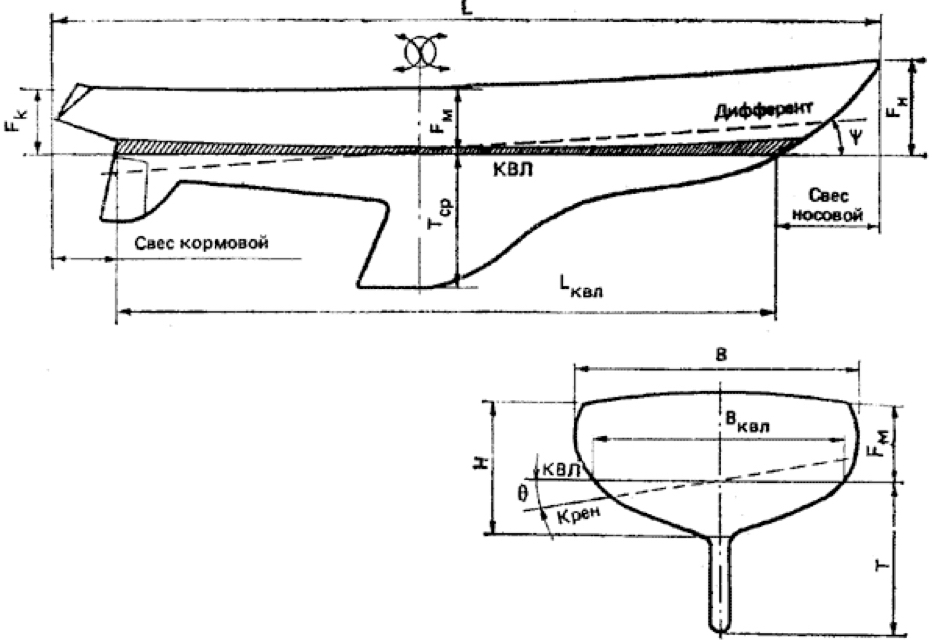
\includegraphics[scale=0.5]{0001_Glavnye_razmereniya_yakhty.jpg}
   \caption{Главные размерения яхты}
   \label{fig:1}
\end{figure}

\begin{description}
\item [Длина наибольшая\index{Длина наибольшая}] (в проектной документации судов она обозначается $L$) \--- расстояние по горизонтали, измеренное между крайними точками по обшивке судна.
\item [Длина по конструктивной ватерлинии\index{Длина по конструктивной ватерлинии} (\textit{КВЛ})] (\lkvl) \--- расстояние между крайними точками корпуса, измеренное по зеркалу воды при полной нагрузке судна либо при другой характерной нагрузке, например в состоянии обмера (см.~гл.~\ref{chap:4}).
\item [Ширина наибольшая\index{Ширина наибольшая}] ($B$) \--- измеряется в самом широком месте судна.
\item [Ширина по КВЛ\index{Ширина по конструктивной ватерлинии}] (\bkvl) \--- наибольшая ширина, измеренная в плоскости ватерлинии.
\item [Высота надводного борта\index{Высота надводного борта}] ($F$) \--- измеряется от ватерлинии до верхней кромки палубного настила у борта. Различают минимальный надводный борт \cidx{F}{М}, надводный борт в носу \cidx{F}{А} (измеряется по отвесу, опущенному из самой крайней точки форштевня) и надводный борт в корме \cidx{F}{К} (по отвесу, опущенному из крайней кормовой точки пересечения линии палубы с поверхностью транца).
\item [Осадка средняя\index{Осадка средняя}] (\tsr) \--- углубление судна, измеренное в средней части \--- на миделе \--- от ватерлинии до нижней кромки фальшкиля. На яхтах с длинной килевой линией измеряют еще максимальную осадку \--- от ватерлинии до самой нижней точки киля, обычно расположенной вблизи пятки руля.
\item [Полная высота борта на миделе\index{Полная высота борта на миделе}] ($H$) измеряется от верхней плоскости балластного фальшкиля до верхней кромки палубного настила у борта. Вместе с $L$ и $B$ высота борта используется в правилах постройки и классификации яхт в качестве параметра для назначения размеров поперечного сечения деталей набора корпуса, элементов якорного устройства и т.\=,п. 
\end{description}

Кроме главных размерений корпуса существуют еще габаритные размеры, например длина вместе с бушпритом, высота от нижней точки киля до верхней точки надстройки, ширина вместе с выступающими снаружи обшивки буртиками или привальным брусьями и т.\=,п.

Главные размерения яхты определяются из условий обеспечения требуемых мореходных качеств, внутреннего расположения жилых и служебных помещений, часто с целью получить определенный гоночный балл или класс. Они являются одними из основных количественных элементов, характеризующих эксплуатационные качества судна \--- его мореходность, вместимость и обитаемость.

Кроме абсолютных цифр судостроители и моряки часто оперируют безразмерными характеристиками \--- соотношениями главных размерений. Наиболее употребительными являются следующие.

\begin{description}
\item [Отношение длины по ватерлинии к ширине\index{Отношение длины по ватерлинии к ширине}] $\lkvl / \bkvl$ \--- характеризует ходкость судна (чем больше $ \lkvl / \bkvl$, тем легче на ходу, быстроходнее судно) и остойчивость (чем меньше $ \lkvl / \bkvl$, тем остойчивее яхта). У современных крейсерско-гоночных яхт, построенных по правилам IOR, $L/B = 2,5 \motdo 5,0$, у крейсерских швертботов $L/B = 2,8 \motdo 3,8$. 
\item [Отношение ширины по КВЛ к осадке\index{Отношение ширины по КВЛ к осадке}] $\bkvl / \tsr$ \--- характеризует ходкость, остойчивость и мореходность. Чем больше $\bkvl / \tsr$, тем остойчивее судно, однако его способность сохранять скорость при волнении оказывается ниже, чем у более узкой и глубокосидящей яхты. Яхты с классическими обводами корпусов имели $\bkvl / \tsr = 1,2 \motdo 1,6$; у современных крейсерско\-/гоночных яхт $\bkvl / \tsr = 1,8$. Для современных килевых яхт с выраженным плавниковым килем более характерно отношение $\bkvl / \tsr$, т.\=,е. ширины по КВЛ к осадке корпуса (без киля). 
\item [Отношение наибольшей длины к высоте борта\index{Отношение наибольшей длины к высоте борта}] $L/H$ \--- характеризует прочность и жесткость корпуса. Чем отношение меньше, тем большей продольной жесткостью обладает корпус, тем меньше он деформируется на волне и от тяги штагов. 
\end{description}

Теоретический чертеж яхты представляет сложную криволинейную наружную поверхность корпуса в виде проекций на три взаимно перпендикулярные плоскости. На этих проекциях изображаются следы пересечения наружной обшивки с секущими плоскостями, положение которых определяется в соответствии с установившимися в судостроении правилами. Три плоскости \--- диаметральная, основная и плоскость мидель-шпангоута являются базовыми плоскостями для построения теоретического чертежа и для постройки судна; они используются в качестве координатных плоскостей, от которых отсчитывают все размеры при последующей модернизации яхты.

\begin{description}
\item [Диаметральная плоскость\index{Диаметральная плоскость}] (\textit{ДП}) \--- вертикальная продольная плоскость симметрии, разделяющая корпус яхты на правую и левую половины. 
\item [Основная плоскость\index{Основная плоскость}] (\textit{ОП}) \--- горизонтальная плоскость, проходящая через самую нижнюю точку киля. Линия пересечения основной плоскости с \textit{ДП} называется основной линией (\textit{ОЛ}). 
\item [Плоскость мидель-шпангоута\index{Плоскость мидель-шпангоута}] (\textbf{миделя}\index{мидель}) \--- вертикальная поперечная плоскость, проходящая посередине длины яхты по КВЛ. Эту плоскость обозначают значком миделя \--- \midelsign. При оценке формы корпуса принято считать миделем самый большой по площади погруженной части шпангоут. 
\end{description}

Три проекции теоретического чертежа получаются сечением корпуса плоскостями, параллельными перечисленным трем базовым плоскостям. Боковая проекция (\textbf{<<бок>>}) образуется в результате сечения корпуса равноотстоящими друг от друга плоскостями, параллельными \textit{ДП}. Показанные на ней кривые линии сечений называются \textbf{батоксами}. Аналогичным образом получаются две другие проекции \--- \textbf{<<полуширота>>} и \textbf{<<корпус>>}. Первая образуется сечениями корпуса плоскостями, параллельными \textit{ОП} \--- \textbf{ватерлиниями}, вторая \--- сечением корпуса плоскостями, параллельными миделю \--- \textbf{шпангоутами}. На <<боку>> и <<полушироте>> шпангоуты изображаются в виде прямых линий; на <<корпусе>> они криволинейные. Ватерлинии выглядят в виде прямых на <<боку>> и <<корпусе>>, а батоксы \--- на <<полушироте>> и <<корпусе>> (рис.~\ref{fig:2}). Прямые линии на каждой проекции образуют сетку теоретического чертежа (на примере яхты <<Симфония>>, конструктор Филипп Брайан, Франция, $L=9,5m$; $B=3,25m$; $F=1,02m$; $T=1,88m$; $V=5,14t$ (???).

\begin{figure}[htb]
   \centering
   \includegraphics{0002_Teor_chertezh}
   \caption{Теоретический чертеж яхты <<Симфония>>}
   \label{fig:2}
   \centering{}\small  1\==10 \--- шпангоуты, Тр \--- транец, ЛБ \--- линия борта, Б1\==Б3 \--- батоксы, ВЛ1\==ВЛ6 \--- ватерлинии, Д \--- диагональ, или рыбина).
\end{figure}

На теоретическом чертеже кроме упомянутых линий батоксов, шпангоутов и ватерлиний изображают очертания плавниковых килей, рулей, транца, фальшборта и т.\=,п. Так как корпус симметричен относительно \textit{ДП}, то на полушироте изображают ватерлинии только левого борта; на проекции <<Бок>> по правую сторону от линии \textit{ДП} вычерчивают обводы носовых шпангоутов, а по левую \--- обводы кормовых.

Все линии теоретического чертежа должны быть согласованы. Это значит, что любая точка на поверхности корпуса должна отстоять на равных расстояниях, например от \textit{ДП} на всех трех проекциях. При согласовании линий конструктор обычно проверяет положение точек пересечения кривых линий с прямыми линиями сетки. Для дополнительного согласования обводов корпуса на теоретическом чертеже проводят рыбины или диагонали \--- следы сечения корпуса продольными, наклонными к \textit{ДП} плоскостями, проведенными через характерные точки на проекции <<корпус>> \--- скулу, вогнутость при киле и т.\=,п. Диагонали проводятся только на <<корпусе>>, в виде прямых линий, и на полушироте вниз от \textit{ДП}, где они имеют вид плавных кривых линий.

Опытному глазу каждая из линий теоретического чертежа может многое сказать о качествах судна. Например, плавные стройные ватерлинии с острым входом в носу и не слишком крутой кривизной в корме благоприятны для хорошего обтекания корпуса водой, как и диагонали аналогичного вида. Батоксы с плавным и пологим \--- под углом $15 \motdo 20\gr$ к \textit{КВЛ} выходом над ватерлинией также важны для плавного, без завихрений, обтекания корпуса. Шпангоуты с явно выраженной скулой и переходом днища в борта по малому радиусу свидетельствуют о высокой начальной остойчивости яхты. В носовой части V-образные шпангоуты с острой вершиной при киле и плавным расширением к палубе важны для сохранения скорости на взволнованном море и незаливаемости палубы. 

Существенное влияние на обводы корпуса оказывают \textbf{Правила обмера}, по которым строится яхта. Так, в 70-х годах в результате введенного в правила обмера IOR, замера глубины трюма (расстояний от \textit{КВЛ} до внутренней поверхности обшивки) на миделе в трех местах по ширине яхты появились суда с трапециевидными шпангоутами. Эти же Правила дали жизнь принципиально новым обводам корпусов \--- с короткими свесами оконечностей, <<обратным>> наклоном транца, высоким надводным бортом и плавниковым килем, которые значительно отличаются от классических яхтенных обводов, господствовавших до конца 60-х годов.

Важнейшей характеристикой яхты является её \textbf{объемное водоизмещение} $V$, т.\=,е. объем воды, вытесняемый яхтой при её погружении по \textit{КВЛ}. Объемное водоизмещение яхты вместе с её главными размерениями позволяет судить о величине судна, его вместимости и потенциальных мореходных качествах. При сравнении яхт часто пользуются безразмерной характеристикой \--- \textbf{коэффициентом полноты водоизмещения} или \textbf{коэффициентом общей полноты} $\delta$, связывающим линейные размеры корпуса с его погруженным объемом. Этот коэффициент определяется как отношение объемного водоизмещения к объему параллелепипеда, имеющего стороны, равные \lkvl, \bkvl и \tsr (рис.~\ref{fig:3}): 

\begin{equation}
\delta = \frac{V}{(\lkvl \cdot \bkvl \cdot  \tsr)}
\end{equation}

\begin{figure}[htb]
   \centering
   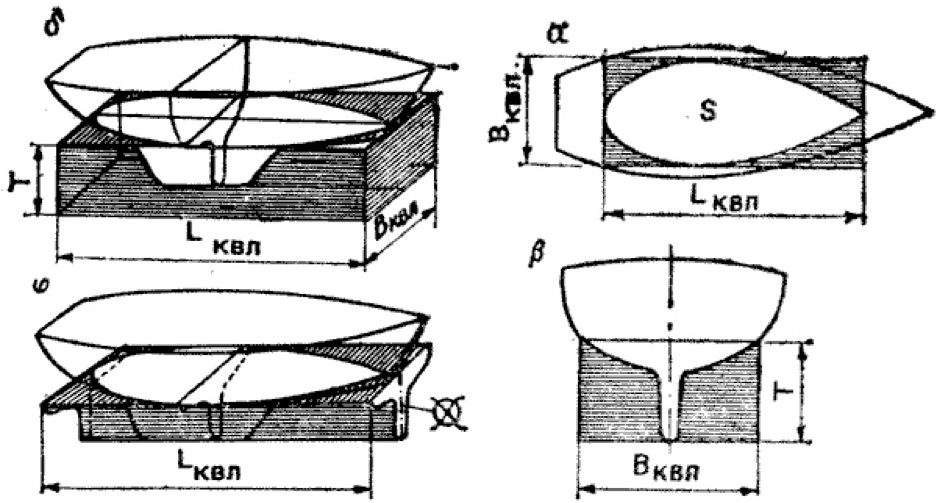
\includegraphics[scale=0.5]{0003_Koeff_polnoty.jpg}
   \caption{Коэффициенты полноты}
   \label{fig:3}
   \centering{}\small $\delta$ \--- водоизмещения; $\alpha$ \--- ватерлинии; $\varphi$ \--- продольной полноты; $\beta$ \--- полноты мидель-шпангоута
\end{figure}

Чем меньше коэффициент общей полноты, тем более острые обводы имеет яхта, тем она быстроходнее. С другой стороны, при уменьшении $\delta$ соответственно уменьшается и полезный объем корпуса ниже ватерлинии, что вызывает необходимость для размещения кают достаточной высоты увеличивать высоту борта или делать более высокие надстройки. Парусные яхты относят к наименее полным судам. Коэффициент общей полноты для крейсерско-гоночных яхт составляет $\delta = 0,15 \motdo 0,22$, для крейсерских швертботов $\delta = 0,26 \motdo 0,35$. Корпуса шхерных крейсеров имели $\delta = 0,12 \motdo 0,15$, в то время как для большинства грузовых коммерческих судов характерна величина $\delta = 0,82$.

К числу безразмерных коэффициентов, характеризующих форму корпуса яхты, относятся также \textbf{коэффициенты полноты площадей ватерлинии} $\alpha$ и \textbf{мидель-шпангоута} $\beta$. Первый представляет собой отношение площади ватерлинии $S$ к прямоугольнику со сторонами  \lkvl и \bkvl: 

\begin{equation}
  \alpha = \frac{S}{\lkvl \cdot \bkvl} \quad ;
\end{equation}

второй \--- отношение площади погруженной части миделя \midelsign к прямоугольнику, стороны которого равны \bkvl и \tsr: 

\begin{equation}
\beta =  \frac{\midelsign}{\bkvl \cdot \tsr}
\end{equation}

Коэффициент $\alpha$, равный для большинства крейсерских яхт 0,70\otdo 0,72, для швертботов 0,60\otdo 0,67, показывает, насколько заострена \textit{КВЛ} в оконечностях, и какую роль в начальной остойчивости яхты играет форма её корпуса. С увеличением полноты ватерлинии повышается остойчивость, но несколько ухудшается обтекаемость корпуса и его ходкость на волне, особенно при большой осадке.

\textbf{Коэффициент продольной полноты} (или \textbf{призматический}) $\varphi$, который представляет собой отношение объемного водоизмещения к объему призмы, имеющей основанием погруженную часть миделя, а высотой длину яхты по КВЛ служит для оценки сопротивления воды движению яхт: 

\begin{equation}
\varphi = \frac{V}{\midelsign \cdot \lkvl}
\end{equation}

Призматический коэффициент, характеризуя распределение погруженного объема корпуса по длине, оказывает существенное влияние на ту часть энергии ветра, которая затрачивается на преодоление волнового сопротивления корпуса. Оптимальная величина $\varphi$ зависит от того, на какую скорость рассчитывается яхта. Если речь идет об очень быстроходных судах, то $\varphi$ принимается близким к $\varphi \approx 0,62$. Для яхт проектируемых на слабые ветра, $\varphi = 0,52 \motdo 0,53$.

\section{Плавучесть, осадка и дифферент}

\textbf{Плавучесть} \--- способность судна держаться на плаву, имея заданную осадку при определенной нагрузке. Это качество должно сохраняться в любых обстоятельствах эксплуатации яхты. 

На погруженную в воду поверхность судна при его неподвижном состоянии в каждой точке действуют силы гидростатического давления воды, направленные перпендикулярно поверхности. Все эти силы можно привести к одной силе плавучести, направленной вверх и приложенной в центре тяжести погруженного объема \--- \textbf{центре величины}, \textit{ЦВ}. Согласно известному закону Архимеда, сила плавучести равна массе воды, вытесненной судном.

Кроме давления воды на корпус судна действуют силы тяжести, которые также могут быть приведены к одной равнодействующей силе $D$, направленной вниз и приложенной в \textbf{центре тяжести}, \textit{ЦТ} судна. Для того чтобы судно плавало в состоянии равновесия, необходимо, чтобы сила плавучести и сила тяжести были равны и располагались на одной вертикали: 

\begin{equation}
  D = \gamma \cdot V
\end{equation}

\begin{equation}
  \cidx{X}{Д} = \cidx{X}{С}
\end{equation}

где $\gamma$ \--- плотность воды, $\mbox{т}/\mbox{м}^3$; $V$ \--- объемное водоизмещение, $\mbox{м}^3$; $D$ \--- масса судна или массовое водоизмещение, т; \cidx{X}{Д} \--- отстояние центра тяжести, \textit{ЦТ}, от плоскости миделя, м; \cidx{X}{С} \--- отстояние центра величины, \textit{ЦВ} от плоскости миделя, м.

В зависимости от плотности воды, в которой плавает яхта, её объемное водоизмещение может изменяться, хотя масса судна остается постоянной. В пресной воде, плотность которой близка к единице, для поддержания судна определенной массы требуется больший погруженный объем V, чем в соленой воде, плотность которой колеблется от $\gamma = 1,010 \motdo 1,015 \, \mbox{т}/\mbox{м}^3$ в Балтийском море до $1,023 \motdo 1,028 \, \mbox{т}/\mbox{м}^3$ в океане. Изменение объемного водоизмещения при переходе яхты из пресной воды ($\gamma = 1,00$) в морскую и наоборот происходит за счет изменения осадки. Величина этого изменения невелика \--- менее 1\% осадки и на эксплуатационных качествах яхты практически не сказывается. Однако влияние солености на осадку следует учитывать при обмере яхты и вычислении её гоночного балла. 

Знание главных размерений яхты и её коэффициентов полноты позволяет капитану выполнять некоторые элементарные расчеты приближенных значений водоизмещения, изменения осадки при приеме груза относительно небольшой величины. 

Водоизмещение:
\begin{equation}
D = \gamma \cdot \delta \cdot \lkvl \cdot \bkvl \cdot \tsr, \mbox{т.} 
\end{equation}

Груз, изменяющий осадку на 1 см:

\begin{equation}
  p = 0,01 \cdot \gamma \cdot \alpha \cdot \lkvl \cdot \bkvl, \mbox{т.}
\end{equation}


\begin{longtable}{p{0.5\textwidth}c}
  \toprule
  Наименование раздела массовой нагрузки & Массовое водоизмещение, \% \\
  \midrule
  Корпус & 30--43 \\
  \midrule
  Фальшкиль & 30--45 \\
  \midrule
  Дельные вещи в корпусе и на палубе & 2--4,5 \\
  \midrule
  Оборудование помещений & 3--7 \\
  \midrule
  Рангоут, такелаж и паруса & 4--7 \\
  \midrule
  Двигатель с трубопроводами и электрооборудованием & 0--7 \\ 
  \midrule
  Системы с трубопроводами и цистернами & 2--4 \\
  \midrule
  Полезная нагрузка: экипаж с багажом, запасы пресной воды, провизии и топлива & 6--8 \\
  \bottomrule
  Массовое водоизмещение & $D = 100\%$ \\
   \caption{Примерное распределение массового водоимещения между разделами нагрузки для крейсерско-гоночных яхт длиной 10\--14 метров}
   \label{tab:1}
\end{longtable}

Если при проектировании или постройке яхты окажется, что её масса превышает водоизмещение по \textit{КВЛ}, а \textit{ЦТ} смещен в нос или корму от \textit{ЦВ}, то при спуске на воду она погрузится глубже конструктивной ватерлинии и получит наклон \--- \textbf{дифферент} на нос или на корму. При продольном наклонении в воду погружается дополнительный объем корпуса в носу или корме и в ту же сторону смещается точка приложения равнодействующей сил плавучести (\textit{ЦВ}) до того момента, пока вновь не будет достигнуто условие плавания в состоянии равновесия т.\=,е. $\cidx{X}{Д} = \cidx{X}{С}$.

И увеличение осадки, и дифферент нежелательны, так как обводы ватерлиний яхты могут существенно отличаться от тех, что были предусмотрены её посадкой по проектной \textit{КВЛ}. Чтобы этого не случилось, после выбора главных размерений конструктор должен хотя бы приблизительно оценить массу будущей яхты. Для этого выполняется предварительный расчет массовой нагрузки по основным разделам: корпус; дельные вещи и палубное оборудование; оборудование внутренних помещений; рангоут, такелаж и паруса; двигатель с трубопроводами, гребным валом и электрооборудованием; системы с трубопроводами, цистернами; полезная нагрузка \--- экипаж, запасы пресной воды и провизии топливо для двигателя, снабжение; балластный фальшкиль. Примерное соотношение этих составляющих массовой нагрузки дано в табл.~\ref{tab:1}, а сумма их должна быть равна массово водоизмещению яхты по \textit{КВЛ}.

Существенное влияние на дифферент яхты оказывают переменные массы \--- топливо и вода в цистернах, которые расходуются в течение плавания, а также экипаж, имеющий возможность перемещаться по яхте. Поэтому цистерны для жидкостей стараются располагать вблизи общего ЦТ яхты, а экипаж во время гонки рассредоточивать на палубе и в помещениях, не допуская его скопления в кормовом кокпите, где масса людей создает значительный дифферентующий момент на корму.

\section{Непотопляемость}

Способность судна оставаться на плаву и сохранять свои мореходные качества в случае получения пробоины в обшивке или затопления через палубные отверстия называется \textbf{непотопляемостью}. Это свойство в первую очередь определяется запасом плавучести судна \--- его надводным объемом от \textit{КВЛ} до палубы. Чем выше надводный борт, тем больше запас плавучести, тем большее количество воды может влиться внутрь яхты, прежде чем она затонет.

Непотопляемость безбалластных швертботов и небольших яхт обеспечить сравнительно несложно. Благодаря легкой конструкции корпуса разность между массой яхты и силой поддержания в аварийном состоянии невелика. Требуется лишь небольшой дополнительный запас плавучести в виде междудонного пространства, бортовых отсеков плавучести, герметичных отсеков в носу и корме, под кокпитом. Для большей надежности эти отсеки заполняют легким пенистым пластиком, не впитывающим воду. Объем отсеков плавучести или блоков пенопласта рассчитывают так, чтобы при заполнении водой яхта держалась на плаву с надводным бортом около 10\,см и по возможности на ровном киле. Чтобы она сохраняла свою способность сопротивляться крену и дифференту, отсеки плавучести размещают в оконечностях корпуса и по бортам. 

Обеспечить непотопляемость крупной яхты, снабженной фальшкилем массой 40\--50\% её водоизмещения и имеющей большой объем внутренних помещений, практически невозможно. В данном случае помогло бы деление корпуса поперечными водонепроницаемыми переборками на несколько отсеков. Однако глухие переборки создают большие неудобства для обитаемости яхт, а при устройстве дверей переборки теряют смысл. Поэтому даже на больших яхтах устанавливают две водонепроницаемые переборки \--- форпиковую (вблизи носового конца \textit{КВЛ}) и ахтерпиковую (в районе кокпита), ограничивающие доступ воды внутрь при получении пробоины в оконечностях. 

Опыт, однако, показывает, что в море от пробоин при столкновениях яхты гибнут сравнительно редко. Гораздо большую опасность представляет негерметичность закрытий палубных люков, разбитые иллюминаторы. Именно это стало причиной гибели пяти яхт в трагической Фастнетской гонке 1979\,г. у берегов Ирландии. На этих яхтах (так же как и еще на 98 из 234 участвовавших в гонке судов) причиной попадания больших масс воды внутрь корпуса были ненадежные закрытия входных люков в стенках рубок. Традиционные задвижные щитки выскакивали из своих пазов при опрокидывании яхт, оказывались смытыми за борт или затерявшимися внутри яхт.

Современная практика требует, чтобы яхта, положенная парусами на воду, не могла быть залита через открытые люки. Входные люки предписывается оборудовать дверцами на прочных петлях, открываемыми обязательно наружу. Все иллюминаторы и светлые люки должны снабжаться защитными щитками, которые в штормовых условиях устанавливаются снаружи. Все отверстия в корпусе для забора забортной воды или выпуска сточных вод, воды из системы охлаждения двигателя и т.\=,п. снабжаются надежными запорными вентилями и клапанами, а осушительная система должна иметь достаточную производительность.

Современная крейсерско-гоночная яхта обладает большой живучестью, т.\=,е. способностью оставаться при аварии на плаву и перемещаться в нужном направлении. В упомянутой Фастнетской гонке на гребнях крутых волн опрокинулось 77 яхт, многие из которых совершили полный оборот на 360\gr. Несмотря на повреждения и большие массы воды, попавшие внутрь яхт, большинство из них были приведены в порты-убежища своими экипажами. Экипажи шести яхт, посчитавшие положение критическим, покинули их на надувных спасательных плотах, которые в тех условиях оказались недостаточно надежными. В результате погибло семь человек. В то же время только две из покинутых шести яхт действительно утонули. Четыре судна, несмотря на жестокий шторм, остались на плаву и были впоследствии обнаружены в море и отбуксированы в гавани.

\section{Силы, действующие на корпус и паруса яхты}

\begin{wrapfigure}{O}{0.5\textwidth}%
  \centering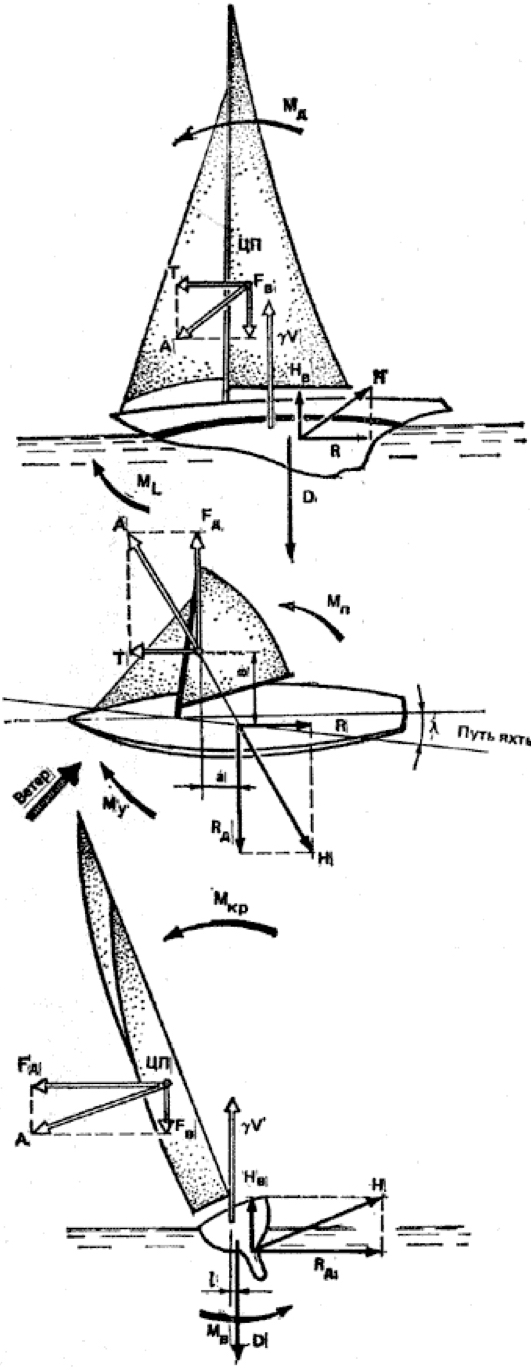
\includegraphics[scale=0.35]{0004_Sily_deistv_na_yakhtu.jpg}
  \caption{Схема сил, действующих на корпус и паруса яхты}
  \label{fig:4}
\end{wrapfigure}

До сих пор мы рассматривали действие на яхту только двух сил \--- силы плавучести и силы веса, предполагая, что она находится в равновесии состоянии покоя. Но поскольку для движения вперед на яхте используются паруса, на судно действует сложная система сил. Схематически она представлена на рис.~\ref{fig:4}, где рассматривается наиболее типичный случай движения яхты в бейдевинд.

При обтекании парусов воздушным потоком \--- ветром \--- на них создается результирующая \textbf{аэродинамическая сила} \textbf{А}, направленная примерно перпендикулярно поверхности паруса и приложенная в центре парусности (\textit{ЦП}) высоко над поверхностью воды. Согласно третьему закону механики, при установившемся движении тела по прямой каждой силе, приложенной к телу, в данном случае \--- к парусам, связанным с корпусом яхты через мачту, стоячий такелаж и шкоты, должна противодействовать равная ей по величине и противоположно направленная сила. На яхте \--- это результирующая \textbf{гидродинамическая сила} \textbf{Н}, приложенная к подводной части корпуса. Таким образом, между этими силами существует известное расстояние \--- плечо, вследствие чего образуется момент пары сил.

И аэро- и гидродинамическая силы оказываются ориентированными не в плоскости, а в пространстве, поэтому при изучении механики движения яхты рассматривают проекции этих сил на главные координатные плоскости. Имея в виду упомянутый третий закон Ньютона, выпишем попарно все составляющие аэродинамической силы и соответствующие им гидродинамические реакции (см. таб.~\ref{tab:1-1}).

\begin{longtable}{cp{0.3\textwidth}cp{0.3\textwidth}}
  \toprule
  Сила & Описание & Сила & Описание \\
  Момент & & Момент & \\
  \midrule
    $\ve{A}$ & Проекция аэродинамической результирующей силы & 
    $\ve{H}$ & Проекция гидродинамической результирующей силы \\
    $\ve{T}$ & Сила тяги, движущая яхту вперед &
    $\ve{R}$ & Сила сопротивления воды движению яхты \\
    $\vidx{F}{Д}$ & Кренящая сила или сила дрейфа &
    $\vidx{R}{Д}$ & Боковая сила или сила сопротивления дрейфу \\
    $\vidx{F}{В}$ & Вертикальная (аэродинамическая) сила &
    $\vidx{H}{В}$ & Вертикальная гидродинамическая сила \\
    $\ve D$ & Сила веса яхты &
    $\gammaV$ & Сила плавучести \\
    $\ve{M}_D$ & Дифферентующий момент &
    $\ve{M}_Z$ & Момент сопротивления дифференту \\
    $\vidx{M}{КР}$ & Кренящий момент &
    $\vidx{M}{В}$ & Восстанавливающий момент \\
    $\vidx{M}{П}$ & Приводящий к ветру момент &
    $\vidx{M}{У}$ & Уваливающий момент \\
  \bottomrule
  \caption{Составляющие аэродинамической силы и соответствующие им гидродинамические реакции}
  \label{tab:1-1}
\end{longtable}

Для того чтобы яхта устойчиво шла по курсу, каждая пара сил и каждая пара моментов сил должны быть равны друг другу. Например, сила дрейфа \vidx{F}{Д}, и сила сопротивления дрейфу \vidx{R}{Д} создают кренящий момент  \vidx{M}{КР}, который должен быть уравновешен восстанавливающим моментом \vidx{M}{В} или моментом поперечной остойчивости. \vidx{M}{В} образуется благодаря действию сил веса \ve{D} и плавучести яхты \ve V, действующих на плече $l$. Эти же силы веса и плавучести образуют момент сопротивления дифференту или момент продольной остойчивости $\ve{M}_l$, равный по величине и противодействующий дифферентующему моменту $\ve M_D$. Слагаемыми последнего являются моменты пар сил $\ve T - \ve R$ и $\vidx{F}{В} - \vidx{H}{В}$. 

В приведенную схему действия сил существенные поправки вносит, особенно на легких яхтах, экипаж. Перемещаясь на наветренный борт или по длине яхты, экипаж своим весом эффективно откренивает судно или противодействует его дифференту на нос. В создании уваливающего момента  \vidx{M}{У} решающая роль принадлежит соответствующему отклонению руля.

Аэродинамическая боковая сила  \vidx{F}{Д}, кроме крена вызывает боковой снос \--- дрейф, поэтому яхта движется не строго по \textit{ДП}, а с небольшим углом дрейфа $l$. Именно это обстоятельство обусловливает образование на киле яхты силы сопротивления дрейфу \vidx{R}{Д}, которая по своей природе аналогична подъемной силе, возникающей на крыле самолета, располагаемом под углом атаки к набегающему потоку. Аналогично крылу работает на курсе бейдевинд и парус, для которого углом атаки является угол между хордой паруса и направлением вымпельного ветра. Таким образом, в современной теории корабля парусная яхта рассматривается как симбиоз двух крыльев: корпуса, движущегося в воде, и паруса, на который воздействует вымпельный ветер.

\section{Остойчивость}

Как мы уже говорили, яхта подвержена действию сил и моментов сил, стремящихся наклонить её в поперечном и продольном направлениях. Способность судна противостоять действию этих сил и возвращаться в прямое положение после прекращения их действия называется \textbf{остойчивостью}. Наиболее важной для яхты является \textbf{поперечная остойчивость}.

\begin{figure}[htb]
   \centering
   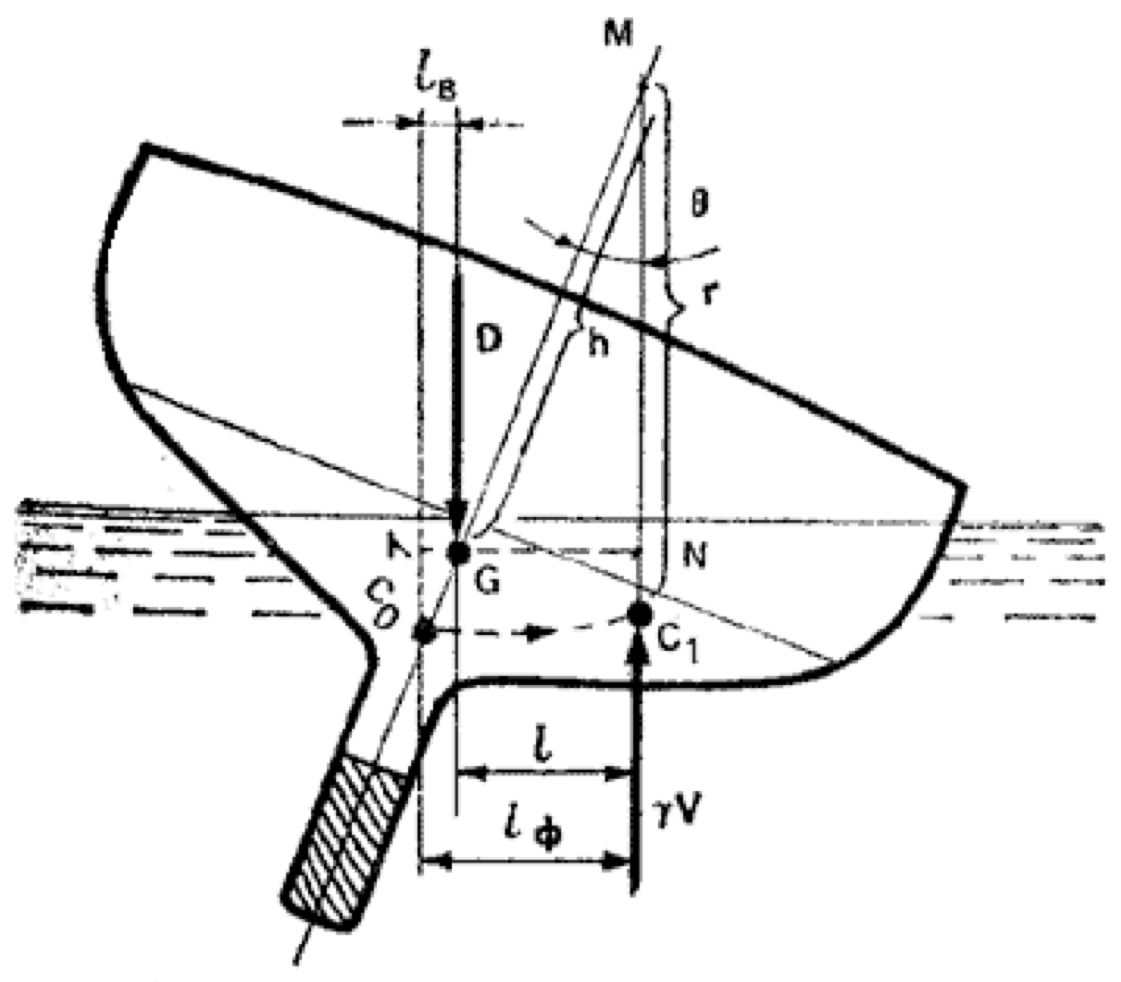
\includegraphics[scale=0.3]{0005_Ostoichevost.jpg}
   \caption{Остойчивость килевой яхты}
   \label{fig:5}
   \centering{}\small Плечо остойчивости $l = \cidx{l}{Ф} - \cidx{l}{В}$
\end{figure}

Когда яхта плавает без крена, то силы тяжести и плавучести, приложенные соответственно в \textit{ЦТ} и \textit{ЦВ}, действуют по одной вертикали. Если при крене экипаж либо другие составляющие массовой нагрузки не перемещаются, то при любом отклонении \textit{ЦТ} сохраняет свое первоначальное положение в \textit{ДП} (точка $G$ на рис.~\ref{fig:5}), вращаясь вместе с судном. В то же время вследствие изменившейся формы подводной части корпуса \textit{ЦВ} смещается из точки $С_0$ в сторону накрененного борта до положения $C_1$. Благодаря этому возникает момент пары сил \ve D и \gammaV с плечом $l$, равным горизонтальному расстоянию между \textit{ЦТ} и новым \textit{ЦВ} яхты. Этот момент стремится возвратить яхту в прямое положение и потому называется \textbf{восстанавливающим}.

При крене ЦВ перемещается по кривой траектории $C_0C_1$, радиус кривизны $r$ которой называется \textbf{поперечным метацентрическим радиусом}, а соответствующий ему центр кривизны $M$ \--- \textbf{поперечным метацентром}. Величина радиуса $r$ и соответственно форма кривой $C_0C_1$ зависят от обводов корпуса. В общем случае при увеличении крена метацентрический радиус уменьшается, так как его величина пропорциональна четвертой степени ширины ватерлинии. 

Очевидно, что плечо восстанавливающего момента зависит от расстояния $GM$ \--- возвышения метацентра над центром тяжести: чем оно меньше, тем соответственно меньше при крене и плечо $l$. На самой начальной стадии наклона величины $GM$ или $h$ рассматривается судостроителями как мера остойчивости судна и называется \textbf{начальной поперечной метацентрической высотой}. Чем больше $h$, тем необходима большая кренящая сила, чтобы наклонить яхту на какой-либо определенный угол крена, тем остойчивее судно. На крейсерско\-/гоночных яхтах метацентрическая высота составляет обычно 0,75\otdo 1,2\,м; на крейсерских швертботах \--- 0,6\otdo 0,8\,м. 

По треугольнику $GMN$ легко установить, что восстанавливающее плечо:

\begin{equation}
  l = G \cdot N = h \cdot \sin \Theta
\end{equation}

Восстанавливающий момент, учитывая равенство \gammaV и \ve D, равен:

\begin{equation}
  \cidx{M}{В} = D \cdot h \cdot \sin \Theta
\end{equation}

Таким образом, несмотря на то, что метацентрическая высота изменяется в довольно узких пределах для яхт различных размерений, величина восстанавливающего момента прямо пропорциональна водоизмещению яхты, следовательно, более тяжелое судно оказывается в состоянии выдержать кренящий момент большей величины.

Восстанавливающее плечо можно представить как разность двух расстояний (см. рис.~\ref{fig:5}): \cidx{l}{Ф} \--- плеча остойчивости формы и \cidx{l}{В} \--- плеча остойчивости веса. Нетрудно установить физический смысл этих величин, так как \cidx{l}{В} определяется отклонением при крене линии действия силы веса от первоначального положения точно над $C_0$, а \cidx{l}{Ф} \--- смещением на подветренный борт центра величины погруженного объема корпуса. Рассматривая действие сил \ve D и \gammaV относительно $C_0$, можно заметить, что сила веса \ve D стремится накренить яхту еще больше, а сила \gammaV, наоборот \--- выпрямить судно. 

\begin{figure}[htb]
  \centering
  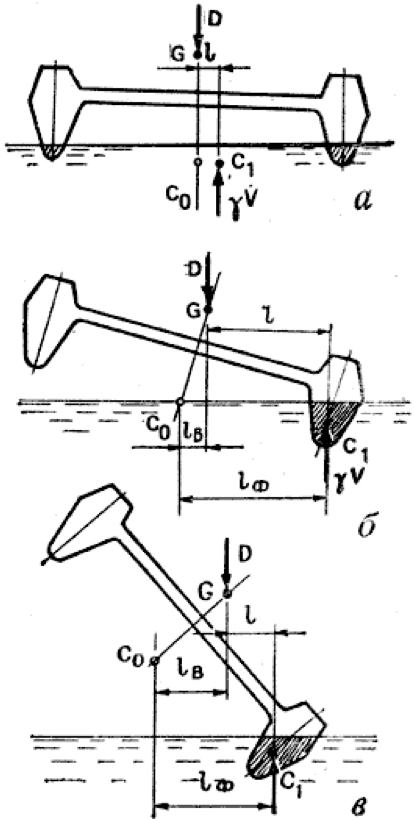
\includegraphics[scale=0.5]{0006_katamaran.jpg}
  \caption{Остойчивость катамарана}
  \label{fig:6}
\end{figure}

По треугольнику $C_0GK$ можно найти, что 

\begin{equation}
  \cidx{l}{В} = G \cdot K = C_0 \cdot G \cdot \sin \Theta \quad , 
\end{equation}

где $C_0 \cdot G$ \--- возвышение \textit{ЦТ} над \textit{ЦВ} в прямом положении яхты. Таким образом, для того чтобы уменьшить отрицательное действие сил веса, необходимо по возможности понизить \textit{ЦТ} яхты. В идеальном случае \textit{ЦТ} должен бы расположиться ниже \textit{ЦВ}, тогда плечо остойчивости веса становится положительным и масса яхты помогает ей сопротивляться действию кренящего момента. Однако только немногие яхты имеют такую характеристику: углубление \textit{ЦТ} ниже \textit{ЦВ} связано с применением очень тяжелого балласта, превышающего 60\% водоизмещения яхты, чрезмерным облегчением конструкции корпуса, рангоута и такелажа. Эффект, аналогичный снижению \textit{ЦТ}, дает перемещение экипажа на наветренный борт. Если речь идет о легком швертботе, то экипажу удается сместить общий \textit{ЦТ} настолько, что линия действия силы \ve D пересекается с \textit{ДП} значительно ниже \textit{ЦВ} и плечо остойчивости веса получается положительным.

У килевой яхты благодаря тяжелому балластному фальшкилю центр тяжести находится достаточно низко (чаще всего \--- под ватерлинией или слегка выше нее). Остойчивость яхты всегда положительная и достигает максимума при крене около 90\gr, когда яхта лежит парусами на воде. Разумеется, такой крен может быть достигнут только на яхте с надежно закрытыми отверстиями в палубе и с самоотливным кокпитом. Яхта с открытым кокпитом может быть залита водой при гораздо меньшем угле крена (яхта класса <<Дракон>>, например, при 52\gr) и пойти ко дну не успев выпрямиться.

У мореходных яхт положение неустойчивого равновесия наступает при крене около 130\gr, когда мачта уже находится под водой, будучи направленной, вниз под углом 40\gr к поверхности. При дальнейшем увеличении крена плечо остойчивости становится отрицательным, опрокидывающий момент способствует достижению второго положения неустойчивого равновесия при крене 180\gr (вверх килем), когда \textit{ЦТ} оказывается расположенным высоко над \textit{ЦВ} достаточно небольшой волны, чтобы судно приняло вновь нормальное положение \--- вниз килем. Известно немало случаев, когда яхты совершали полный оборот на 360\gr и сохраняли свои мореходные качества. 

Сравнивая остойчивость килевой яхты и швертбота, можно заметить, что главную роль в создании восстанавливающего момента у швертбота играет остойчивость формы, а у килевой яхты \--- остойчивость веса. Поэтому и существует столь заметная разница в обводах их корпусов: швертботы имеют широкие корпуса с $L/B = 2,6 \motdo 3,2$, со скулой малого радиуса и большой полнотой ватерлинии. В еще большей степени форма корпуса определяет остойчивость катамаранов, у которых объемное водоизмещение разделено поровну между двумя корпусами. Уже при небольшом крене водоизмещение между корпусами резко перераспределяется, увеличивая силу плавучести корпуса, погружающегося в воду (рис.~\ref{fig:6}). Когда другой корпус выходит из воды (при крене 8\otdo 15\gr), плечо остойчивости достигает максимальной величины \--- оно немного меньше половины расстояния между \textit{ДП} корпусов. При дальнейшем увеличении крена катамаран ведет себя подобно швертботу, экипаж которого висит на трапеции. При крене 50\otdo 60\gr наступает момент неустойчивого равновесия, после чего остойчивость катамарана становится отрицательной.

\begin{figure}[htb]
  \centering
  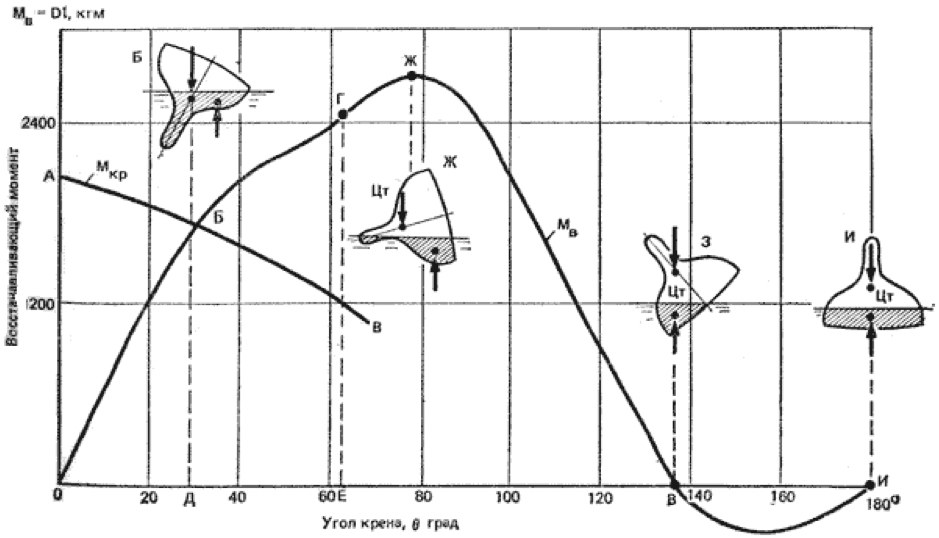
\includegraphics[scale=0.5]{0007_Diag_stat_ost.jpg}
  \caption{Диаграмма статической остойчивости крейсерско-гоночной яхты}
  \label{fig:7}
\end{figure}

\textbf{Диаграмма статической остойчивости}. Очевидно, что полной характеристикой остойчивости яхты может быть кривая изменения восстанавливающего момента \vidx{M}{В} в зависимости от угла крена $\Theta$ или диаграмма статической остойчивости (рис.~\ref{fig:7}). На диаграмме хорошо различимы моменты максимума остойчивости (Ж) и предельного угла крена, при котором судно, будучи предоставлено само себе, опрокидывается (З \--- угол заката диаграммы статической остойчивости).

С помощью диаграммы капитан судна имеет возможность оценивать, например, способность яхты нести ту или, иную парусность при ветре определенной силы. Для этого на диаграмму остойчивости наносят кривые изменения кренящего момента \vidx{M}{КР} в зависимости от угла крена $\Theta$. Точка Б пересечения обеих кривых указывает на угол крена, который получит яхта при статическом, с плавным нарастанием действии ветра. На рис.~\ref{fig:7} яхта получит крен, соответствующий точке Д, \--- около 29\gr. Для судов, имеющих явно выраженные нисходящие ветви диаграммы остойчивости (швертботов, компромиссов и катамаранов), плавание может, быть допущено только при углах крена, не превышающих точки максимума на диаграмме остойчивости. 

На практике экипажам яхт приходится нередко иметь дело с динамическим действием внешних сил, при котором кренящий момент достигает значительной величины в сравнительно короткий промежуток времени. Такое бывает при шквале или ударе волны в наветренную скулу. В этих случаях важна не только величина кренящего момента, но и кинетическая энергия, сообщаемая судну и поглощаемая работой восстанавливающего момента. 

На диаграмме статической остойчивости работа обоих моментов может быть представлена в виде площадей, заключенных между соответствующими кривыми и осями ординат. Условием равновесия яхты при динамическом воздействии внешних сил будет равенство площадей ОАБВЕ (работа \vidx{M}{КР}) и ОБГВЕ (работа \vidx{M}{В}). Учитывая, что площади ОБВЕ общие, можно рассматривать равенство площадей ОАБ и БГВ. На рис.~\ref{fig:7} видно, что в случае динамического действия ветра угол крена (точка Е, около 62\gr) заметно превышает крен от ветра такой же силы при его статическом действии. 

По диаграмме статической остойчивости может быть определен \textbf{предельный динамический кренящий момент}, опрокидывающий швертбот или угрожающий безопасности яхты с открытым кокпитом. Очевидно, что действие восстанавливающего момента может рассматриваться только до угла заливания кокпита или до начальной точки снижения диаграммы статической остойчивости.

Принято считать, что килевые яхты, снабженные тяжелым балластом, практически неопрокидываемы. Однако в уже упоминавшейся Фастнетской гонке 1979\,г. 77 яхт были опрокинуты на угол крена более 90\gr, причем часть из них некоторое время (от 30 сек до 5 мин) оставалась на плаву вверх килем, а несколько яхт встали потом в нормальное положение через другой борт. Наиболее серьезными повреждениями при этом были потери мачт (на 12 яхтах), падение из своих гнезд аккумуляторов, тяжелых камбузных плит и другого оборудования. К нежелательным последствиям привело и попадание воды внутрь корпусов. Случилось это под динамическим воздействием крутой 9--10\-/метровой волны, профиль которой резко ломался при переходе из океана в мелководное Ирландское море, при ветре скоростью 25\otdo 30\,м/с.

\textbf{Факторы, влияющие на поперечную остойчивость}. Таким образом, мы можем сделать определенные выводы о влиянии различных элементов проекта яхты на её остойчивость. На малых углах крена главную роль в создании восстанавливающего момента играют ширина яхты и коэффициент полноты площади ватерлинии. Чем шире яхта и полнее её ватерлиния, тем дальше от \textit{ДП} смещается \textit{ЦВ} при крене судна, тем больше плечо остойчивости формы. Диаграмма статической остойчивости достаточно широкой яхты имеет более крутую восходящую ветвь, чем узкой, \--- до $\Theta = 60 \motdo 80gr$. 

Чем ниже расположен центр тяжести яхты, тем она остойчивее, причем влияние глубокой осадки и большого балласта сказывается практически по всей диаграмме остойчивости яхты. Занимаясь модернизацией яхты, полезно помнить простое правило: каждый килограмм под ватерлинией повышает остойчивость, а каждый килограмм над ватерлинией ухудшает её. Особенно ощутим для остойчивости тяжелый рангоут и такелаж.

При одинаковом расположении центра тяжести яхта с избыточным надводным бортом имеет и более высокую остойчивость на углах крена более 30\otdo 35\gr, когда на судне с нормальной высотой борта палуба начинает входить в воду. Высокобортная яхта имеет большую величину максимального восстанавливающего момента. Это качество присуще также яхтам, имеющим водонепроницаемые рубки достаточно большого объема. 

Особо следует остановиться на влиянии воды в трюме и жидкостей в цистернах. Дело не только в перемещении масс жидкостей в сторону накрененного борта; главную роль играет наличие свободной поверхности переливающейся жидкости, а именно \--- её момент инерции относительно продольной оси. Если, например, поверхность воды в трюме имеет длину $l$, а ширину $b$, то метацентрическая высота уменьшается на величину

\begin{equation}
  \Delta h = \frac{l \cdot b^3}{\ 12D\ }, \quad \text{м.}
\end{equation}

Особенно опасна вода в трюме, свободная поверхность которого имеет большую ширину. Поэтому при плавании в штормовых условиях воду из трюма нужно своевременно удалять.

Для уменьшения влияния свободной поверхности жидкостей в цистернах устанавливают продольные отбойные переборки, которые по ширине делят на несколько частей. В переборках делают отверстия для свободного перетекания жидкости.

\textbf{Поперечная остойчивость и ходкость яхты.} При увеличении крена сверх 10\otdo 12\gr сопротивление воды движению яхты заметно возрастает, что приводит к потере скорости. Поэтому важно, чтобы при усилении ветра яхта дольше могла нести эффективную парусность, не имея чрезмерного крена.Нередко даже на сравнительно крупных яхтах во время гонок экипаж располагается на наветренном борту, пытаясь уменьшить крен. 

Насколько эффективно перемещение груза (экипажа) на один борт, нетрудно представить по простейшей формуле, которая справедлива для небольших углов (в пределах 0\otdo 10\gr) крена:

\begin{equation}
  \vidx{M}{О} = \frac{D \cdot h}{57,3} \quad ,
\end{equation}

где: \vidx{M}{O} \--- момент, кренящий яхту на 1\gr; $D$ \--- водоизмещение яхты, т; $h$ \--- начальная поперечная метацентрическая высота, м. 

Зная массу перемещаемого груза и расстояние нового места расположения его от \textit{ДП}, можно определить кренящий момент, а разделив его на \vidx{M}{О}, получить угол крена в градусах. Например, если на яхте водоизмещением 7\,т при $h=1\,\text{м}$ пять человек расположатся у борта на расстоянии 1,5\,м от \textit{ДП}, то создаваемый ими кренящий момент придаст яхте крен в 4,5\gr (или уменьшит примерно на столько же крен на другой борт). 

\textit{Продольная остойчивость.} Физика явлений, происходящих при продольных наклонах яхты аналогична явлениям при крене, но продольная метацентрическая высота по величине сравнима с длиной яхты. Поэтому продольные наклоны, дифферент, обычно невелики и измеряются не в градусах, а по изменениям осадки носом и кормой. И, тем не менее, если из яхты выжимают все её возможности, нельзя не считаться с действием сил, дифферентующих яхту на нос и перемещающих центр величины, вперед (см. рис.~\ref{fig:4}). Этому можно противодействовать, перемещая экипаж в кормовую часть палубы. 

Наибольшей величины дифферентующие на нос силы достигают при плавании в бакштаг; на этом курсе, особенно в сильный ветер, экипаж следует смещать, возможно, дальше в корму. На курсе бейдевинд дифферентующий момент невелик, и экипажу лучше всего располагаться близ миделя, откренивая судно. На фордевинде дифферентующий момент оказывается меньше, чем на бакштаге, особенно если яхта несет спинакер и блупер, дающие определенную подъемную силу.

У катамаранов величина продольной метацентрической высоты сравнима с поперечной, иногда меньше нее. Поэтому действие дифферентующего момента, практически незаметное на килевой яхте, может опрокинуть катамаран, таких же главных размерений. Статистика аварий отмечает случаи опрокидывания через нос на попутных курсах крейсерских катамаранов с высокой парусностью. 

\section{Сопротивление дрейфу}

Поперечная сила \vidx{F}{Д} (см. рис.~\ref{fig:4}) не только кренит яхту, она вызывает боковой снос \--- \textbf{дрейф под ветер}. Сила дрейфа зависит от курса яхты относительно ветра. При плавании в крутой бейдевинд она втрое превышает силу тяги, движущую яхту вперед; на галфвинде обе силы примерно равны; в крутой бакштаг (истинный ветер около 135\gr относительно курса яхты) движущая сила оказывается в 2--3 раза больше силы дрейфа, а на чистом фордевинде сила дрейфа вовсе отсутствует. Следовательно, для того чтобы судно успешно продвигалось вперед курсом от бейдевинда до галфвинда, оно должно обладать достаточным боковым сопротивлением дрейфу, намного превышающим сопротивление воды движению яхты по курсу. 

Функцию создания силы сопротивления дрейфу у современных яхт выполняют в основном шверты, плавниковые кили и рули. 

Как мы уже говорили, непременным условием возникновения силы сопротивления дрейфу является движение яхты под небольшим углом к \textit{ДП} \--- углом дрейфа. Рассмотрим, что при этом происходит в потоке воды непосредственно у киля, который представляет собой крыло с поперечным сечением в виде тонкого симметричного аэродинамического профиля (рис.~\ref{fig:8}).

\begin{figure}[htb]
  \centering
  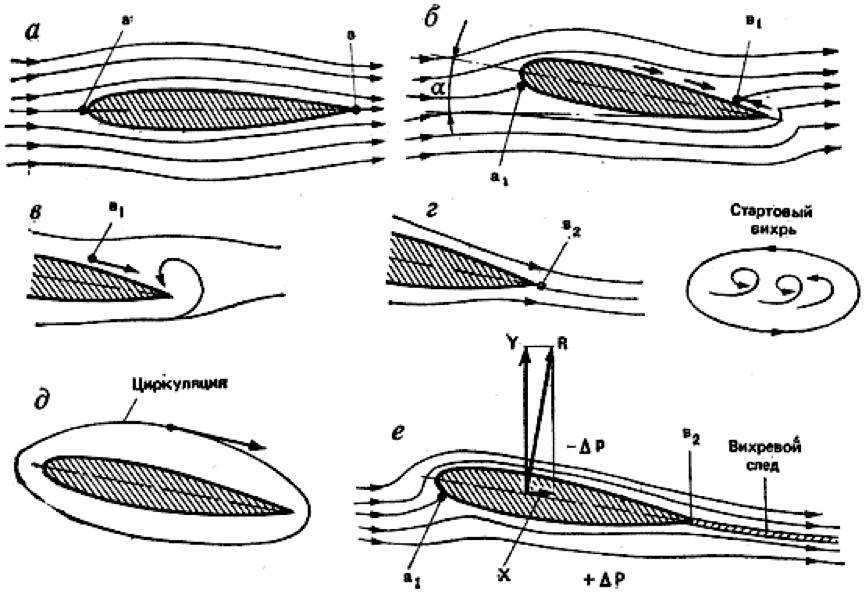
\includegraphics[scale=0.5]{0008_Podemn_sila.jpg}
  \caption{Образование подъемной силы на крыле}
  \label{fig:8}
  \centering{}\small \textit{a} \--- обтекание профиля при $\alpha = 0$;
                     \textit{б}~и~\textit{в} \--- образование стартового вихря;
                     \textit{г} \--- отрыв стартового вихря;
                     \textit{д} \--- появление устойчивой циркуляции потока вокруг крыла;
                     \textit{е} \--- схема действующих сил при развитой циркуляции
\end{figure}

Если угол дрейфа отсутствует (рис.~\ref{fig:8},~\textit{а}), то поток воды, встречаясь с профилем киля в точке \textit{а}, разделяется на две части. В этой точке, называемой критической, скорость потока равна 0, давление максимальное, равное скоростному напору $(\rho \cdot v^2) / 2$, где: $\rho$ \--- массовая плотность воды (для пресной воды = 102 $\text{кгс}^2 / \text{м}^4$ ); $v$ \--- скорость движения яхты (м/с). 

И верхняя и нижняя части потока одновременно обтекают поверхности профиля и вновь встречаются в точке \textit{b} на выходящей кромке. Очевидно, что никакой силы, направленной поперек потока, на профиле возникнуть не может; будет действовать только одна сила сопротивления трения, обусловленная вязкостью воды. 

Если же профиль отклонить на некоторый угол атаки $\alpha$ (в случае яхтенного киля \--- угол дрейфа), то картина обтекания профиля изменится (рис.~\ref{fig:8},~\textit{б}). Критическая точка $a$ переместится на нижнюю часть <<носика>> профиля. Путь, который должна пройти частица воды вдоль верхней поверхности профиля, удлинится, а точка $b_1$, где по условиям неразрывности потока должны были бы встретиться частицы, обтекающие верхнюю и нижнюю поверхности профиля, пройдя равный путь, оказывается на верхней поверхности. Однако при огибании острой выходящей кромки профиля нижняя часть потока срывается с кромки в виде вихря (рис.~\ref{fig:8},~\textit{в} и \textit{г}). Этот вихрь, называемый стартовым, вращаясь против часовой стрелки, вызывает циркуляцию воды вокруг профиля в обратном направлении, т.\=,е. по часовой стрелке (рис.~\ref{fig:8},~\textit{д}). Данное явление, вызванное силами вязкости, аналогично вращению большого зубчатого колеса (циркуляция), находящегося в зацеплении с малой ведущей шестерней (стартовый вихрь). 

После того как возникает циркуляция, стартовый вихрь срывается с выходящей кромки, точка $b_2$ перемещается ближе к этой кромке, вследствие чего здесь больше не существует разности скоростей, с которыми крыло покидают верхняя и нижняя части потока. Циркуляция же вокруг крыла становится причиной возникновения подъемной силы \ve Y, направленной поперек потока: у верхней поверхности крыла скорость частиц воды за счет циркуляции увеличивается, у нижней, встречаясь с частицами, вовлеченными в циркуляцию, \--- затормаживается. Соответственно у верхней поверхности давление понижается по сравнению с давлением в потоке перед крылом, а у нижней поверхности \--- повышается. Разность давлений и дает подъемную силу \ve Y. 

Кроме того, на профиль будет действовать \textbf{сила лобового (профильного) сопротивления} \ve X, возникающая вследствие трения воды о поверхность профиля и гидродинамического давления на его переднюю часть.

\begin{figure}[htb]
  \centering
  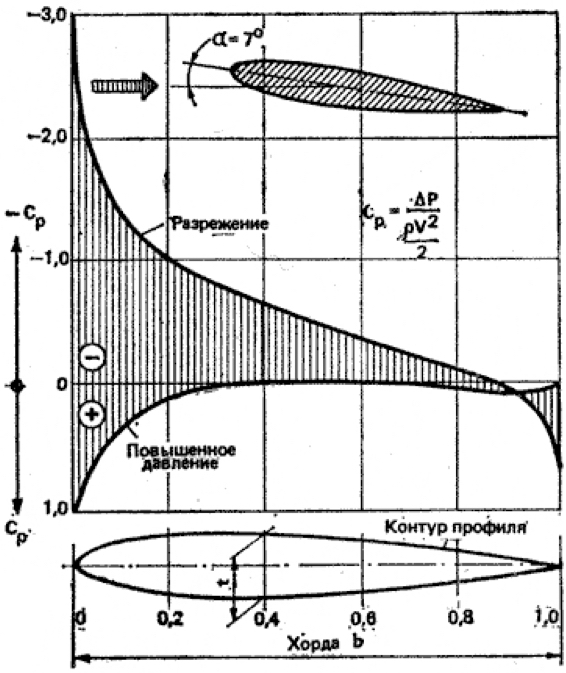
\includegraphics[scale=0.5]{0009.jpg}
  \caption{Распределение давления по ширине симметричного аэродинамического профиля при угле атаки $\alpha = 7\gr$}
  \label{fig:9}
\end{figure}

На рис.~\ref{fig:9} представлены результаты замера давления у поверхности симметричного профиля, сделанного в аэродинамической трубе. По оси ординат отложено значение коэффициента $C_P$, который представляет собой отношение избыточного давления (полное давление минус атмосферное) к скоростному напору $(\rho \cdot v^2) / 2$. На верхней стороне профиля давление отрицательное (разрежение), на нижней \--- положительное. Таким образом, подъемная сила, действующая на любой элемент профиля, складывается из действующих на него сил давления и разрежения, а в целом она пропорциональна площади, заключенной между кривыми распределения давления по хорде профиля (на рис.~\ref{fig:9} заштриховано).

Данные, представленные на рис.~\ref{fig:9}, позволяют сделать ряд важных выводов о работе яхтенного киля. Во-первых, главную роль в создании боковой силы играет разрежение, возникающее на поверхности плавника со стороны наветренного борта. Во-вторых, пик разрежения располагается вблизи входящей кромки киля. Соответственно точка приложения результирующей подъемной силы находится на передней трети хорды плавника. В целом же подъемная сила возрастает вплоть до угла атаки 15\otdo 18\gr, после чего внезапно падает.

Вследствие образования завихрения на стороне разрежения плавное обтекание крыла нарушается, разрежение падает и происходит срыв потока (это явление более подробно рассмотрено в гл.~\ref{chap:2} для парусов). Одновременно с увеличением угла атаки возрастает лобовое сопротивление \--- оно достигает максимума при $\alpha = 90\gr$.

Величина дрейфа современной яхты редко превышает 5\gr, так что срыв, потока с киля можно не опасаться. Однако критический угол атаки должен учитываться для яхтенных рулей, которые проектируются и работают также по принципу крыла. 

Рассмотрим основные параметры яхтенных килей, которые оказывают существенное влияние на их эффективность в создании силы сопротивлению дрейфу. В равной степени изложенное далее можно распространить и на рули с учетом того, что они работают со значительно большим углом атаки.

\textbf{Толщина и форма поперечного сечения киля.} Испытания симметричных аэродинамических профилей показали, что более толстые профили (с большей величиной отношения толщины сечения $t$ к его хорде $b$) дают большую подъемную силу. Их лобовое сопротивление выше, чем у профилей с меньшей относительной толщиной. Оптимальные результаты могут быть получены при $t/b = 0,09 \motdo 0,12$. Величина подъемной силы на таких профилях сравнительно мало зависит от скорости яхты, поэтому кили развивают достаточную силу сопротивления дрейфа и в слабый ветер. 

Существенное влияние на величину силы сопротивления дрейфу оказывает положение максимальной толщины профиля по длине хорды. Наиболее эффективными оказываются профили, у которых максимальная толщина расположена на расстоянии 40\otdo 50\% хорды от их <<носика>>. Для яхтенных рулей, работающих под большими углами атаки, используют профили с максимальной толщиной, расположенной несколько ближе к передней кромке, \--- до 30\% хорды.

Определенное влияние на эффективность киля оказывает форма, <<носика>> профиля \--- радиус округления входящей кромки. Если кромка слишком острая, то набегающий на киль поток получает здесь большое ускорение и срывается с профиля в виде вихрей. При этом происходит падение подъемной силы, особенно существенное при больших углах атаки. Поэтому подобное заострение входящей кромки недопустимо для рулей. 

\textbf{Аэродинамическое удлинение.} У концов крыла обнаруживается перетекание воды из области повышенного давления на спинку профиля. В результате с концов крыла срываются вихри, образующие две вихревые дорожки. На их поддержание затрачивается довольно значительная часть энергии, образуя так называемое \textbf{индуктивное сопротивление}. Кроме того, вследствие выравнивания давлений у концов крыла происходит местное падение подъемной силы, как это показано на эпюре распределения её по длине крыла на рис.~\ref{fig:10}. 

\begin{figure}[htb]
  \centering
  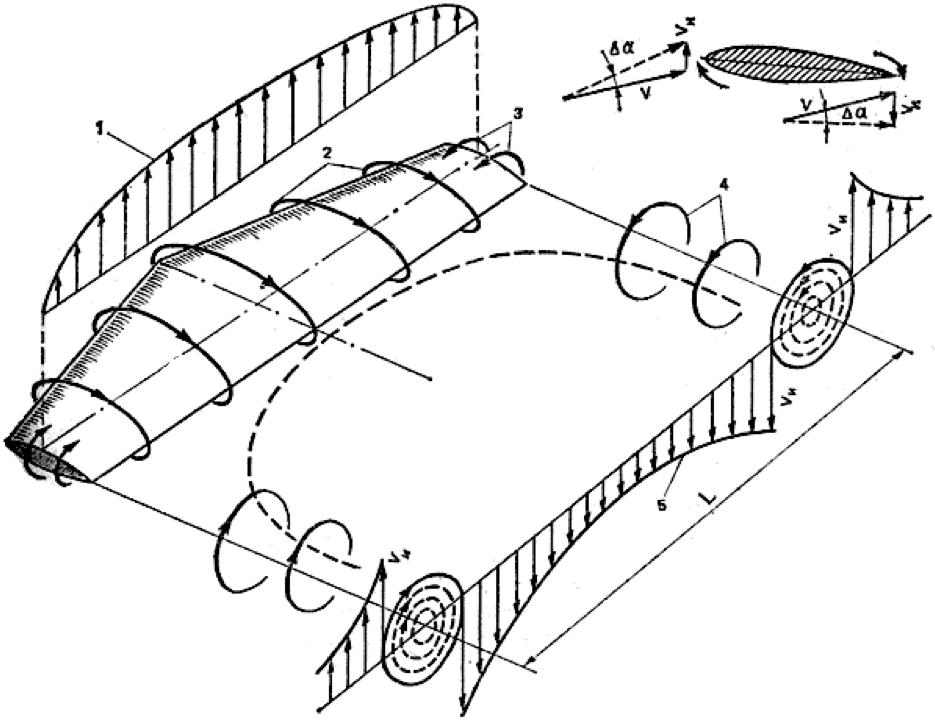
\includegraphics[scale=0.5]{0010.jpg}
  \caption{Схема обтекания крыла конечного размаха}
  \label{fig:10}
  \centering
  \small
  \textit{1} \--- распределение подъемной силы по длине крыла;
  \textit{2} \--- циркуляция;
  \textit{3} \--- перетекание жидкости по концам крыла;
  \textit{4} \--- концевые вихри;
  \textit{5} \--- распределение вызванных скоросте по размаху крыла $L$
\end{figure}

Чем короче длина крыла $L$ по отношению к его хорде $b$, т.\=,е. чем меньше его удлинение $L/b$, тем относительно больше потеря подъемной силы и тем больше индуктивное сопротивление. В аэродинамике принято оценивать удлинение крыла по формуле $\lambda = L^2/S$ (где $S$ \--- площадь крыла), которая может быть применена для крыльев и плавников любых очертаний. При прямоугольной форме аэродинамическое удлинение равно соотношению $\lambda = L / b$; для треугольного крыла $\lambda = 2 \cdot L / b$.
На рис.~\ref{fig:10} показано крыло, составленное из двух трапециевидных плавниковых килей. На яхте киль крепится широким основанием к днищу, поэтому здесь перетекание воды на сторону разрежения отсутствует и под влиянием корпуса давления на обоих поверхностях выравнивается. Без этого влияния можно было бы считать аэродинамическое удлинение вдвое большим, чем отношение глубины киля к его осадке. На практике же это отношение, зависящее от размеров киля, обводов яхты и угла крена превышается только в 1,2\otdo 1,3 раза.

\begin{figure}[htb]
  \centering
  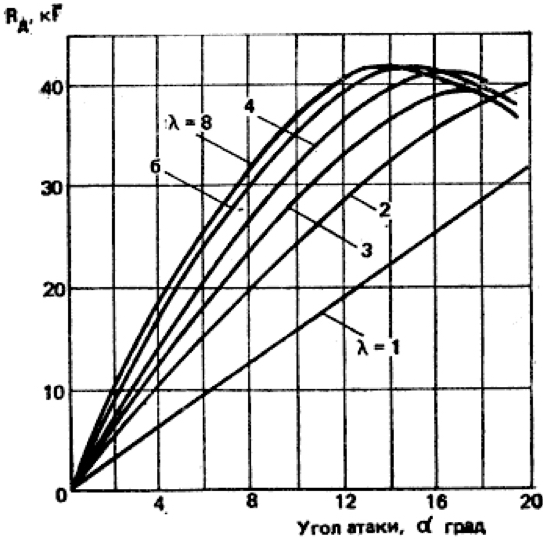
\includegraphics[scale=0.5]{0011.jpg}
  \caption{Зависимость сопротивления дрейфу от удлинения и угла атаки}
  \label{fig:11}
\end{figure}

Влияние аэродинамического удлинения киля на величину развиваемой им силы сопротивления дрейфу \vidx{R}{Д} можно оценить по результатам испытаний плавника, имеющего профиль NACA 009 ($t/b = 9\%$) и площадь 0,37\,м$^2$ (рис.~\ref{fig:11}). Скорость потока соответствовала скорости движения яхты 3 узла (1,5\,м/с). Интерес представляет изменение силы сопротивления дрейфу при угле атаки 4\otdo 6\gr, что соответствует углу дрейфа яхты на курсе бейдевинд. Если принять силу \vidx{R}{Д} при удлинении $\lambda = 1$ за единицу (6,8 при $\alpha = 5\gr$), то при увеличении $\lambda$ до 2 сопротивление дрейфу увеличивается более чем в 1,5 раза (10,4\,кг), а при $\lambda = 3$ \--- ровно вдвое (13,6\,кг). Этот же график может служить для качественной оценки эффективности рулей различного удлинения, которые работают в области больших углов атаки.

Таким образом, увеличивая удлинение плавника киля, можно получить необходимую величину боковой силы \vidx{R}{Д} при меньшей площади киля и, следовательно, при меньшей площади смоченной поверхности и сопротивлении воды движению яхты. Удлинение килей на современных крейсерско\-/гоночных яхтах составляет в среднем $\lambda = 1 \motdo 3$. Перо руля, служащее не только для управления судном, но и являющееся составным элементом в создании сопротивления яхты, имеет еще большее удлинение, приближающееся к $\lambda = 4$. 

\textbf{Площадь и формы киля.} Чаще всего размеры киля определяют по статистическим данным, сравнивая проектируемую яхту с хорошо зарекомендовавшими себя судами. На современных крейсерско\-/гоночных яхтах с раздельным от киля рулем суммарная площадь киля и руля составляет от 4,5 до 6,5\% площади парусности яхты, а площадь руля \--- 20\otdo 40\% площади киля.

Для получения оптимального удлинения конструктор яхты стремится принять осадку наибольшей допускаемой по условиям плавания или правилами обмера. Чаще всего киль имеет вид трапеции с наклонной передней кромкой. Как показали исследования, для яхтенных килей, имеющих удлинение от 1 до 3, угол между передней кромкой и вертикалью в пределах от -8\gr до 22,5\gr практически не влияет на гидродинамические характеристики киля. Если киль (или шверт) очень узкий и длинный, то наклон передней кромки более 15\gr к вертикали сопровождается отклонением линий тока воды вниз по профилю \--- по направлению к нижнему заднему углу. Вследствие этого падает подъемная сила и возрастает лобовое сопротивление киля. В данном случае оптимальный угол наклона составляет 5\gr к вертикали. 

На величину подъемной силы, развиваемой килем и рулем, значительно влияет качество отделки его поверхности, особенно передней кромки, где формируется поток, обтекающий профиль. Поэтому рекомендуется полировать киль и руль на расстоянии не менее 1,5\% хорды профиля.

\textbf{Скорость яхты.} Подъемная сила на любом крыле определяется по формуле:

\begin{equation}
  \ve Y = C_Y \cdot \frac{\rho \cdot v^2}{2} \cdot S, \text{кгс,} 
\end{equation}

где: $C_Y$ \--- коэффициент подъемной силы, зависящий от параметров крыла \--- формы профиля, удлинения, очертаний в плане, а также от угла атаки \--- с увеличением угла атаки он возрастает; $\rho$ \--- массовая плотность воды, кгс$^2$/м$^4$; $v$ \--- скорость потока, обтекающего крыло, м/с; $S$ \--- площадь крыла, м$^2$.
 
Таким образом, сила сопротивления дрейфу \--- величина переменная, пропорциональная квадрату скорости. В начальный момент движения яхты, например, после поворота оверштаг, когда судно теряет ход, или при отходе от бона в прижимной ветер, подъемная сила на киле невелика. Для того чтобы сила \ve Y сравнялась с силой дрейфа \vidx{F}{Д}, киль должен расположиться к набегающему потоку под большим углом атаки. Иными словами, судно начинает движение с большим углом дрейфа. По мере набора скорости угол дрейфа уменьшается, пока не достигнет своей нормальной величины \--- 3\otdo 5\gr.

Это обстоятельство должен учитывать капитан, предусматривая достаточно места с подветра при разгоне яхты или после поворота на новый галс. Большой начальный угол дрейфа необходимо использовать для скорейшего набора скорости, слегка потравив шкоты. Кстати, благодаря этому уменьшается сила дрейфа на парусах. 

Необходимо также помнить механику возникновения подъемной силы, которая появляется на киле только после отрыва стартового вихря и развития устойчивой циркуляции. На узком киле современной яхты циркуляция возникает быстрее, чем на корпусе яхты с навесным на киле рулем, т.\=,е. на крыле с большой хордой. Вторая яхта больше сдрейфует под ветер, прежде чем корпус начнет эффективно препятствовать дрейфу.

\section{Управляемость}

Управляемостью называется качество судна, позволяющее ему следовать по заданному курсу или изменять направление движения. Управляемой может считаться только та яхта, которая реагирует нужным образом на перекладку руля.

Управляемость объединяет два свойства судна \--- устойчивость на курсе и поворотливость.

\textbf{Устойчивость на курсе} \--- это способность яхты удерживать заданное прямолинейное направление движения при действии на нее различных внешних сил: ветра, волнения и т.\=,п. Устойчивость на курсе зависит не только от конструктивных особенностей яхты и характера действия внешних сил, но и от реакции рулевого на отклонение судна от курса, его чутья руля.

Обратимся вновь к схеме действия внешних сил на паруса и корпус яхты (см. рис.~\ref{fig:4}). Решающее значение для устойчивости яхты на курсе имеет взаимное расположение двух пар сил. Кренящая сила \vidx{F}{Д} и сила сопротивления дрейфу \vidx{R}{Д} стремятся увалить нос яхты под ветер, в то время как вторая пара \--- сила тяги \ve T и сопротивление движению \ve R приводит яхту к ветру. Очевидно, что реакция яхты зависит от соотношения величины рассматриваемых сил и плеч $a$ и $b$, на которых они действуют. При увеличении угла крена плечо приводящей пары $b$ также увеличивается. Плечо уваливающей пары, $a$ зависит от взаимного расположения центра парусности (\textit{ЦП}) \--- точки приложения результирующей аэродинамических сил к парусам и центра бокового сопротивления (\textit{ЦБС}) \--- точки приложения результирующей гидродинамических сил к корпусу яхты. Положение этих точек изменяется в зависимости от многих факторов: курса яхты относительно ветра, формы и настройки парусов, крена и дифферента яхты, формы и профиля киля и руля и т.\=,п.

\begin{figure}[htb]
  \centering
  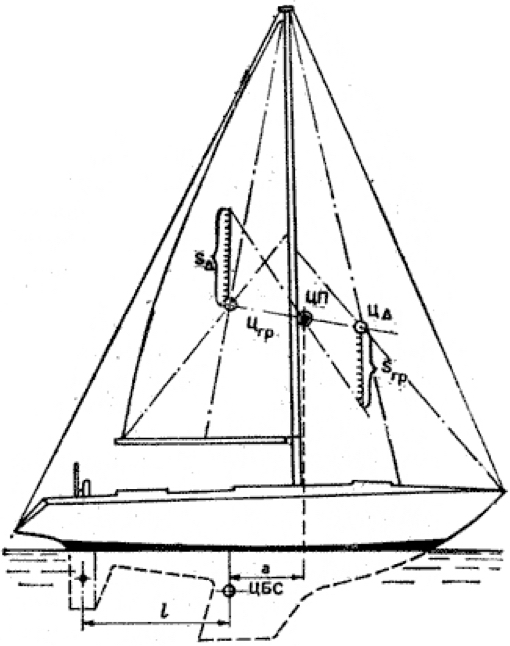
\includegraphics[scale=0.5]{0012.jpg}
  \caption{Схема определения геометрического центра парусности яхты с вооружением типа <<шлюп>>}
  \label{fig:12}
\end{figure}

Поэтому при проектировании и перевооружении яхт оперируют с условными \textit{ЦП} и \textit{ЦБС}, считая их расположенными в центрах тяжести плоских фигур, которыми являются паруса, поставленные в диаметральной плоскости яхты, и подводные очертания \textit{ДП} с килем, плавниками и рулем (рис.~\ref{fig:12}). 

Известно, что центр тяжести треугольного паруса располагается на пересечении двух медиан, а общий центр тяжести двух парусов находится на отрезке прямой, соединяющей \textit{ЦП} обоих парусов, и делит этот отрезок обратно пропорционально их площади. Обычно, в расчет принимается не фактическая площадь стакселя, а обмерная площадь переднего парусного треугольника. 

Положение \textit{ЦБС} можно определить, уравновешивая на острие иголки профиль подводной части \textit{ДП}, вырезанный из тонкого картона. Когда шаблон располагается строго горизонтально, игла находится в условной точке \textit{ЦБС}. Напомним, что в создании силы сопротивления дрейфу главная роль принадлежит плавниковому килю и рулю. Центры гидродинамических давлений на их профилях могут быть найдены достаточно точно, например, для профилей с относительной толщиной $t/b$ около 8\% эта точка находится на расстоянии около 26\% хорды от входящей кромки. Однако корпус яхты, хотя и участвует в создании поперечной силы в малой степени, вносит определенные изменения в характер обтекания киля и руля, причем он изменяется в зависимости от угла крена и дифферента, а также скорости яхты. В большинстве случаев на курсе бейдевинд истинный \textit{ЦБС} перемещается вперед. 

Конструкторы, как правило, располагают \textit{ЦП} на некотором расстоянии (опережении) впереди \textit{ЦБС}. Обычно опережение задается в процентах длины судна по ватерлинии и составляет для бермудского шлюпа 15\otdo 18\% \lkvl.

Если истинный \textit{ЦП} оказывается расположенным слишком далеко впереди \textit{ЦБС}, яхта на курсе бейдевинд уваливается под ветер и рулевому приходится постоянно держать руль отклоненным на ветер. Если же \textit{ЦП} оказывается позади \textit{ЦБС}, то яхта стремится привестись к ветру; требуется постоянная работа рулем, чтобы сдерживать судно. 

Особенно неприятна тенденция яхты к уваливанию. В случае аварии с рулем яхту не удается с помощью одних парусов привести на курс бейдевинд, кроме того, она обладает повышенным дрейфом. Дело в том, что киль яхты отклоняет стекающий с него поток воды ближе к \textit{ДП} судна. Поэтому если руль стоит прямо, он работает с заметно меньшим углом атаки, чем киль. Если отклонить руль в наветренную сторону, то образуемая на нем подъемная сила оказывается направленной в подветренную сторону \--- туда же, что и сила дрейфа на парусах. В данном случае киль и руль <<тянут>> в разные стороны и яхта неустойчива на курсе.

Иное дело легкая тенденция яхты приводиться. Переложенный на небольшой угол (3\otdo 4\gr) под ветер руль работает с таким же или несколько большим углом атаки, что и киль, и эффективно участвует в сопротивлении дрейфу. Поперечная сила, возникающая на руле, вызывает значительное смещение общего \textit{ЦБС} к корме, одновременно уменьшается угол дрейфа, яхта устойчиво лежит на курсе.

Однако если на курсе бейдевинд руль приходится постоянно перекладывать под ветер на большую величину, чем 3\otdo 4\gr, следует подумать о корректировке относительного положения \textit{ЦБС} и \textit{ЦП}. На уже построенной яхте это проще делать, перемещая вперед \textit{ЦП}, \--- устанавливая мачту в степсе в крайнее носовое положение или наклоняя её вперед. Причиной приведения яхты может быть также грот \--- слишком <<пузатый>> или с перебранной задней шкаториной. В этом случае полезен промежуточный штаг, с помощью которого можно придать мачте в средней части (по высоте) прогиб вперед и тем самым сделать парус более плоским, а также ослабить заднюю шкаторину. Можно также укоротить длину нижней шкаторины грота. 

Сложнее сместить в корму \textit{ЦБС}, для чего нужно установить кормовой плавничок перед рулем или увеличить площадь пера руля.

Мы уже говорили, что при увеличении крена увеличивается, и тенденция яхты приводиться. Это происходит не только вследствие увеличения плеча приводящей пары сил \--- \ve T и \ve R. При крене гидродинамическое давление в районе носовой волны повышается, что приводит к смещению \textit{ЦБС} вперед. Поэтому в свежий ветер для уменьшения тенденции яхты приводиться следует переместить вперед и \textit{ЦП}: взять риф на гроте или немного перетравить его для данного курса. Полезно также сменить стаксель на меньший по площади, благодаря чему уменьшается крен и дифферент яхты на нос.

Опытный конструктор при выборе величины опережения а обычно учитывает остойчивость яхты, чтобы компенсировать рост приводящего момента при крене: для яхты с меньшей остойчивостью задается большая величина опережения, для более остойчивых судов опережение принимается минимальным.

Хорошо уцентрованные яхты часто обладают повышенной рыскливостью на курсе бакштаг, когда потравленный на борт грот стремится развернуть яхту носом к ветру. Этому помогает и высокая волна, набегающая с кормы под углом к ДП. Чтобы одерживать яхту на курсе, приходится сильно работать рулем, отклоняя его на критический угол, когда возможен срыв потока с его подветренной поверхности (обычно это случается при углах атаки a 15\otdo 20\gr). Это явление сопровождается потерей подъемной силы на руле и, следовательно, управляемости яхты. Яхта внезапно может резко броситься к ветру и получить большой крен, при этом из-за уменьшения углубления пера руля на сторону разрежения может прорваться воздух с поверхности воды. 

Борьба с этим явлением, получившим название \textbf{брочинг}, заставляет увеличивать площадь пера руля и его удлинение, устанавливать перед рулем плавник, площадь которого составляет около четверти площади пера. Благодаря наличию плавника перед рулем организуется направленный поток воды, увеличиваются критические углы атаки руля, предотвращается прорыв воздуха к нему и уменьшается усилие на румпеле. При плавании в бакштаг экипаж должен стремиться к том чтобы тяга спинакера была направлена по возможности вперед, а не вбок чтобы избежать излишнего крена. Важно также препятствовать появлению дифферента на нос, при котором может уменьшиться углубление руля. Брочингу способствует также бортовая качка яхты, появляющаяся вследствие срывов потока воздуха со спинакера.

Устойчивость на курсе помимо рассмотренного влияния внешних сил и взаимного расположения их точек приложения определяется конфигурацией подводной части \textit{ДП}. Ранее для дальних плаваний по открытой воде отдавали предпочтение яхтам с длинной килевой линией, как обладающим большим сопротивлением повороту и соответственно \--- устойчивостью на курсе. Однако этому типу судов свойственны существенные недостатка например большая смоченная поверхность и плохая поворотливость. К тому же выяснилось, что устойчивость на курсе зависит не столько от величины боковой проекции \textit{ДП}, сколько от положения руля относительно \textit{ЦБС}, т.\=,е. от <<рычага>>, на котором действует руль. Отмечено, что если это расстояние оказывается менее 25\% \lkvl, то яхта становится рыскливой и плохо реагирует на отклонение руля. При $l = 40 \motdo 45\%$ \lkvl (см. рис.~\ref{fig:12}) удержание судна на заданном курсе не составляет труда.

\begin{figure}[htb]
  \centering
  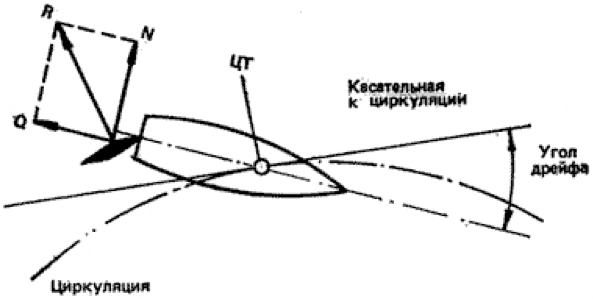
\includegraphics[scale=0.5]{0013.jpg}
  \caption{Действие руля и схема движения яхты на циркуляции}
  \label{fig:13}
\end{figure}

\textbf{Поворотливость} \--- способность судна изменять направление движения, описывать траекторию под действием руля и парусов. Действие руля основано на том же принципе гидродинамического крыла, что рассматривался и для яхтенного киля. При перекладке руля на некоторый угол возникает гидродинамическая сила \ve R, одна из составляющих которой \ve N толкает корму яхты в сторону, противоположную той, в которую положен руль (рис.~\ref{fig:13}). Под её действием судно начинает двигаться по кривой траектории. Одновременно сила \ve R дает составляющую \ve Q \--- силу сопротивления, тормозящую ход яхты.

Если закрепить руль в одном положении, то судно пойдет примерно по окружности, называемой циркуляцией. Диаметр или радиус циркуляции является мерой поворотливости судна: чем больше радиус циркуляции, тем хуже поворотливость. По циркуляции движется только центр тяжести яхты, корму выносит наружу. Одновременно судно получает дрейф, вызванный центробежной силой и отчасти силой \ve N на пере руля.

Радиус циркуляции зависит от скорости и массы яхты, её момента инерции относительно вертикальной оси, проходящей через \textit{ЦТ}, от эффективности руля \--- величины силы \ve N и её плеча относительно \textit{ЦТ} при данном отклонении руля. Чем больше скорость и водоизмещение яхты, чем больше тяжелых масс (двигатель, якоря, детали оборудования) размещено в оконечностях судна, тем больше радиус циркуляции. Обычно радиус циркуляции, определенный на ходовых испытаниях яхты, выражают в длинах корпуса.

Поворотливость тем лучше, чем короче подводная часть судна и чем ближе к миделю сконцентрирована её основная площадь. Плохой поворотливостью обладают, например, суда с длинной килевой линией (типа военно\-/морских шлюпок) и, наоборот, хорошей \--- швертботы с узкими глубокими швертами. 

Эффективность руля зависит от площади и формы пера, профиля поперечного сечения, аэродинамического удлинения, типа установки (на ахтерштевне, отдельно от киля или на плавнике), а также расстояния баллера от \textit{ЦБС}. Наибольшее распространение получили рули, спроектированные в виде крыла с аэродинамическим профилем поперечного сечения. Максимальной толщина профиля принимается обычно в пределах 10\otdo 12\% хорды и располагается на 1/3 хорды от передней кромки. Площадь руля составляет обычно 9,5\otdo 11\% площади погруженной части \textit{ДП} яхты. 

Руль с большим удлинением (отношение квадрата глубины погружения руля к его площади) развивает большую поперечную силу на малых углах атаки, благодаря чему он эффективно участвует в обеспечении боковой силы сопротивления дрейфу. Однако, как было показано на рис.~\ref{fig:11}, на определенных углах атаки профилей различного удлинения происходит отрыв потока от поверхности разрежения, после чего подъемная сила на профиле существенно падает. Например, при $\lambda = 6$ критический угол перекладки руля составляет 15\gr; при $\lambda = 2$ составляет 30\gr. В качестве компромисса применяют рули с удлинением $\lambda = 4 \motdo 5$ (соотношение сторон прямоугольного руля 2\otdo 2,5), а для повышения критического угла перекладки устанавливают перед рулем плавник\-/скег. Руль с большим удлинением быстрее реагирует на перекладку, так как циркуляция потока, обусловливающая подъемную силу, быстрее развивается вокруг профиля с малой хордой, чем вокруг всей подводной части корпуса с навесным на ахтерштевне рулем. 

Верхняя кромка руля должна плотно прилегать к корпусу в пределах рабочих отклонений $\pm 30\gr$, чтобы препятствовать перетеканию воды через нее; в противном случае эффективность работы руля ухудшается. Иногда на пере руля, если он навешен на транце, закрепляют аэродинамическую шайбу в виде широкой пластины близ ватерлинии.

Сказанное о форме килей применимо и к рулям: оптимальной считается трапециевидная форма с прямоугольной либо слегка скругленной нижней кромкой. Для уменьшения усилий на румпеле руль иногда делают балансирного типа \--- с осью вращения, расположенной на 1/4\otdo 1/5 хорды от <<носика>> профиля.

При управлении яхтой необходимо учитывать специфику работы руля в различных условиях, и, прежде всего срыв потока с его спинки. Нельзя делать резких перекладок руля на борт в начале поворота \--- произойдет срыв потока, поперечная сила \ve N на руле упадет, зато быстро увеличится сила сопротивления \ve R. Яхта будет входить в циркуляцию медленно и с большой потерей скорости. Начинать поворот необходимо, переложив руль на небольшой угол, но как только корма покатится наружу, и угол атаки руля начнет уменьшаться, его следует переложить на больший угол относительно \textit{ДП} яхты. 

Следует помнить, что поперечная, сила на руле быстро возрастает с увеличением скорости яхты. В слабый ветер бесполезно пытаться повернуть яхту быстро, перекладывая руль на большой угол (кстати, величина критического угла зависит от скорости: на меньшей скорости отрыв потока происходит при меньших углах атаки).

Сопротивление руля при изменении курса яхты в зависимости от его формы, конструкции и расположения составляет от 10 до 40\% общего сопротивления яхты. Поэтому к технике управления рулем (и к центровке яхты, от которой зависит устойчивость на курсе) надо относиться весьма серьезно, не допускать отклонения руля на больший угол, чем это необходимо.

\section{Ходкость}

\textbf{Ходкостью} называют способность яхты развивать определенную скорость при эффективном использовании энергии ветра.

Скорость, которую может развить яхта, зависит прежде всего от скорости ветра, поскольку все аэродинамические силы, действующие на парус в том числе и сила тяги, возрастав пропорционально квадрату скорости вымпельного ветра. Кроме того, она зависит и от энерговооруженности судна \--- отношения площади парусности к его размерениям. В качестве характеристики энерговооруженности чаще всего применяют отношение $S^{1/2} / V^{1/3}$
(где $S$ \--- площадь парусности м$^2$; $V$ \--- полное водоизмещение, м$^3$); или $S / \Omega$ 
(здесь $\Omega$ \--- смоченная поверхность корпуса, включая киль и руль). Сила тяги, а, следовательно, и скорость яхты, определяется еще и способностью парусного вооружения развивать достаточную тягу на различных курсах по отношению к направлению ветра.

Перечисленные факторы относятся к парусам \--- движителю яхты, преобразующему энергию ветра в движущую силу \ve T. Как было показано на рис.~\ris{4}, эта сила при равномерном движении яхты должна быть равна и противоположно направлена силе сопротивления движению \ve R. Последняя представляет собой проекцию результирующих всех гидродинамических сил, действующих на смоченную поверхность корпуса, на направление движения.

Различают два рода гидродинамических сил: силы давления, направленные перпендикулярно поверхности корпуса, и силы вязкости, действующие по касательной к этой поверхности. Результирующая сил вязкости дает силу \textbf{сопротивления трения}. 

Силы давления обусловлены образованием при движении яхты волн на поверхности воды, поэтому их результирующая дает силу \textbf{волнового сопротивления}. 

При большой кривизне поверхности корпуса в кормовой части пограничный слой может отрываться от обшивки, могут образовываться завихрения, поглощающие часть энергии движущей силы. Так возникает еще одна составляющая сопротивления движению яхты \--- \textbf{сопротивление формы}.

Еще два вида сопротивления появляются в связи с тем, что яхта движется не прямо вдоль \textit{ДП}, а с некоторым углом дрейфа и с креном. Это \textbf{индуктивное} и \textbf{креновое} сопротивления. Существенную долю в индуктивном сопротивлении занимает сопротивление выступающих частей \--- киля и руля.

Наконец, движению яхты вперед оказывает сопротивление и воздух, омывающий корпус, экипаж, развитую систему тросов такелажа и паруса. Эта часть сопротивления носит название \textbf{воздушного}. 

\textbf{Сопротивление трения.} При движении яхты частицы воды, непосредственно примыкающие к обшивке корпуса, как бы прилипают к ней и увлекаются вместе с судном. Скорость этих частиц относительно корпуса равна нулю (рис.~\ris{14}). Следующий слой частиц, скользя по первому, уже немного отстает от соответствующих точек корпуса, а на определенном расстоянии от обшивки вода вообще остается неподвижной или имеет скорость относительно корпуса, равную скорости яхты $v$. Этот слой воды, в котором действуют силы вязкости, а скорость движения частиц воды относительно корпуса возрастает от 0 до скорости судна, называется пограничным слоем. Толщина его относительно невелика и составляет от 1 до 2\% длины корпуса по ватерлинии, однако характер или режим движения частиц воды в нем оказывает существенное влияние на величину сопротивления трения.

\begin{figure}[htb]
  \centering
  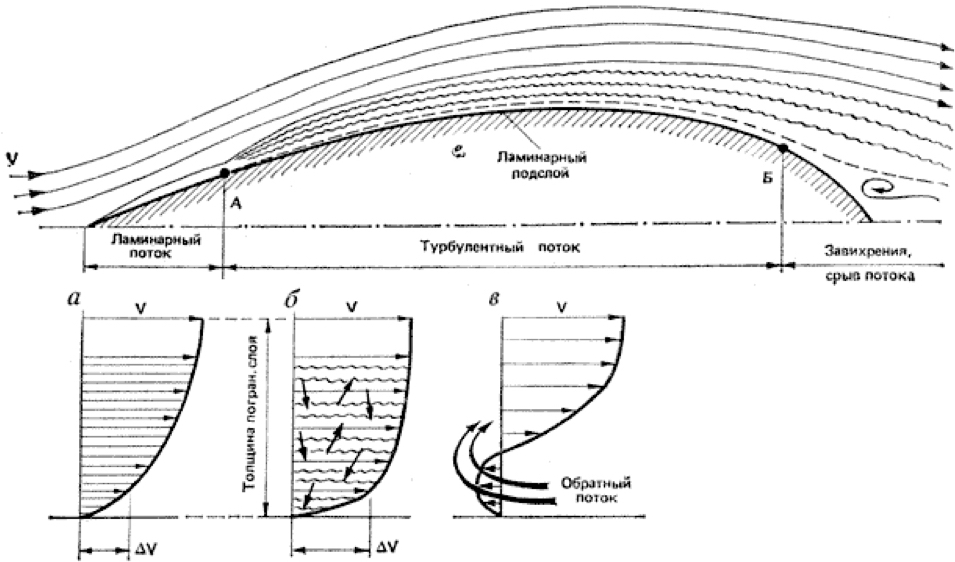
\includegraphics[scale=0.5]{0014.jpg}
  \caption{Потоки жидкости около корпуса яхты}
  \label{fig:14}
\end{figure}

Установлено, что режим движения частиц изменяется в зависимости от скорости судна и длины его смоченной поверхности. В гидродинамике эта зависимость выражается числом Рейнольдса:

\begin{equation}
  \Renum = \frac{v \cdot L}{\nu} \quad , 
\end{equation}

где: $\nu$ \--- коэффициент кинематической вязкости воды (для пресной воды $\nu = 1,15 \cdot 10^{-6} \text{м}^2/\text{с})$; $L$ \--- длина смоченной поверхности, м; $v$ \--- скорость яхты, м/с. 

При относительно небольшом числе $\Renum = 10^{-6}$ (???) частицы воды в пограничном слое движутся слоями, образуя ламинарный поток. Его энергии оказывается недостаточно, чтобы преодолеть силы вязкости, препятствующие поперечным перемещениям частиц. Наибольший перепад скорости между слоями частиц оказывается непосредственно у поверхности корпуса; соответственно и силы трения имеют здесь наибольшую величину. 

Число Рейнольдса в пограничном слое увеличивается по мере удаления частиц воды от форштевня (с возрастанием смоченной длины). При скорости 2 м/с, например, уже на расстоянии около 2 м от него Re достигнет критической величины, при которой режим потока в пограничном слое становится вихревым, т.\=,е. турбулентным и направленным поперек пограничного слоя. Вследствие возникшего обмена кинетической энергией между слоями скорость частиц близ поверхности корпуса растет в большей степени, чем при ламинарном потоке. Перепад скоростей $\Delta v$ здесь возрастает, соответственно растет и сопротивление трения. Вследствие поперечных движений частиц воды толщина пограничного слоя увеличивается, а сопротивление трения резко увеличивается. 

Ламинарный режим обтекания охватывает только небольшую часть корпуса яхты в носовой его части только на малых скоростях. Критическая величина Re, при которой возникает турбулентное обтекание корпуса, лежит в пределах $5 \cdot 10^5\motdo 6 \cdot 10^6$ и в значительной степени зависит от формы и гладкости поверхности его. При повышении скорости точка перехода, ламинарного пограничного слоя в турбулентный перемещается в сторону носа. При достаточно высокой скорости может наступить момент, когда вся смоченная поверхность корпуса будет охвачена турбулентным потоком. Правда, непосредственно около обшивки, где скорость обтекания близка к нулю, все же сохраняется тончайшая пленка с ламинарным режимом \--- ламинарный подслой. 

Сопротивление трения рассчитывают по формуле:

\begin{equation}
  \cidx{R}{ТР} = \cidx{\zeta}{ТР} \cdot \frac{\rho \cdot v^2}{2} \cdot \Omega, \quad \text{кгс}, 
\end{equation}

где: \cidx{R}{ТР} \--- сопротивление трения, кг; \cidx{\zeta}{ТР} \--- коэффициент сопротивления трения; $\rho$ \--- массовая плотность воды; для пресной воды: $\rho = 102\, \text{кг} \cdot \text{с}^2/\text{м}^4$; $v$ \--- скорость яхты, м/с; $\Omega$ \--- смоченная поверхность, м$^2$. 

Коэффициент сопротивления трения \--- величина переменная, зависящая от характера потока в пограничном слое, длины корпуса \lkvl, скорости $v$ и шероховатости поверхности корпуса.

На рис.~\ris{15} показaнa зависимость коэффициента сопротивления трения \cidx{\zeta}{ТР} от числа Re и шероховатости поверхности корпуса.

\begin{figure}[htb]
  \centering
  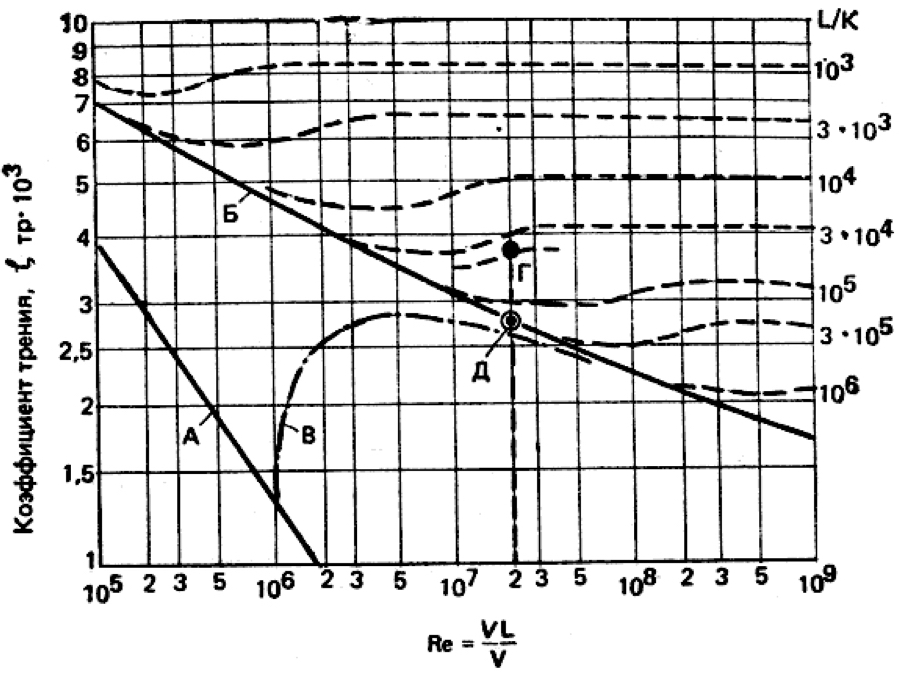
\includegraphics[scale=0.5]{0015.jpg}
  \caption{Зависимость коэффициента сопротивления трения от числа Рейнольдса}
  \label{fig:15}
\end{figure}

Рост сопротивления шероховатой поверхности по сравнению с гладкой нетрудно объяснить наличием в турбулентном пограничном слое ламинарного подслоя. Если бугорки на поверхности полностью погружены в ламинарный подслой, то они не вносят существенных изменений в характер ламинарного течения подслоя. Если же неровности превышают толщину подслоя и выступают над ним, то происходит турбулизация движения частиц воды по всей толщине пограничного слоя, и коэффициент трения соответственно возрастает.

Рис.~\ris{15} позволяет оценить важность отделки днища яхты для снижения её сопротивления трения. Например, если яхта длиной 7,5\,м по ватерлинии идет со скоростью $v = 6$ узл. (3,1\,м/с), то соответствующее число $\Renum = (3,1 \cdot 7,5) / (1,15 \cdot 10^{-6} ) = 2 \cdot 10^7$. 

Допустим, что днище яхты имеет шероховатость (среднюю высоту неровностей) $k = 0,2$\,мм, что соответствует относительной шероховатости $L/k = 7500 / 0,2 = 3,75 \cdot 10^4$.

Для данной шероховатости и числа Rе коэффициент трения равен $\cidx{\zeta}{ТР} = 0,0038$ (точка Г).

Оценим, можно ли получить в данном случае поверхность днища, близкую к технически гладкой. При $\Renum = 2 \cdot 10^7$ такой поверхности соответствует относительная шероховатость $L/k = 3 \cdot 10^5$ или абсолютная шероховатость $k = 7500/3 \cdot 10^5 = 0,025$\,мм. Опыт показывает, что этого можно добиться, тщательно отшлифовав днище мелкой шкуркой, а затем отлакировав его. Оправдаются ли затраченные усилия? График показывает, что коэффициент сопротивления трения снизится до $\cidx{\zeta}{ТР} = 0,0028$ (точка Д), или на 30\%, чем, конечно, не может пренебрегать экипаж, рассчитывающий на успех в гонках.

Линия Б позволяет оценить допустимую шероховатость днища для яхт различных размеров и различной скорости. Можно заметить, что с увеличением длины по ватерлинии и скорости требования к качеству поверхности возрастают. 

Для ориентировки приведем значения шероховатости (в мм) для различных поверхностей:
\begin{itemize}
\item деревянная, тщательно лакированная и шлифованная \--- 0,003\otdo 0,005; 
\item деревянная, окрашенная и шлифованная \--- 0,02\otdo 0,03; 
\item окрашенная патентованным покрытием \--- 0,04\otdo 0,06; 
\item деревянная, окрашенная суриком \--- 0,15; 
\item обычная доска \--- 0,5; 
\item обросшее ракушками днище \--- до 4,0.
\end{itemize}

Мы уже говорили, что на части длины яхты, начиная от форштевня, может сохраняться ламинарный пограничный слой, если только излишняя шероховатость не будет способствовать турбулизации потока. Поэтому особенно важно тщательно обрабатывать носовую часть корпуса, все входящие кромки киля, плавников и рулей. При малых поперечных размеpax \--- хордах (???) следует шлифовать всю поверхность киля и руля. В кормовой части корпуса, где толщина пограничного слоя увеличивается, требования к отделке поверхности могут быть несколько снижены. 

Особенно сильно отражается на сопротивлении трения обрастание днища водорослями и ракушками. Если периодически не очищать днище яхт, постоянно находящихся в воде, то через два--три месяца сопротивление трения может увеличиться на 50\otdo 80\%, что равносильно потере скорости в средний ветер на 15\otdo 25\%. 

\textbf{Сопротивление формы.} Даже у хорошо обтекаемого корпуса на ходу можно обнаружить кильватерный след \--- струю, в которой вода совершает вихревые движения. Это следствие отрыва от корпуса пограничного слоя в определенной точке (Б на рис.~\ris{14}). Положение точки зависит от характера изменения кривизны поверхности по длине корпуса. Чем плавнее обводы кормовой оконечности, тем дальше к корме происходит отрыв пограничного слоя и меньше вихреобразование. 

При нормальных соотношениях длины корпуса к ширине сопротивление формы невелико. Увеличение его может быть обусловлено наличием острых скул, сломов обводов корпуса, правильно спрофилированных килей, рулей и других выступающих частей. Сопротивление формы увеличивается с уменьшением протяженности зоны ламинарного пограничного слоя, этому следует снять наплывы краски, уменьшить шероховатость, заделать выемки в обшивке, поставить обтекатели на выступающие патрубки и т.\=,п.

\textbf{Волновое сопротивление.} Возникновение волн у корпуса судна при движении вызвано действием сил тяжести жидкости на границе раздела воды и воздуха. В носовой оконечности, в месте встречи корпуса с водой, давление резко повышается, и вода поднимается на некоторую высоту. Ближе к миделю, где вследствие расширения корпуса судна скорость обтекающего потока увеличивается, давление в нем, согласно закону Бернулли, падает, и уровень воды понижается. В кормовой части, где давление вновь повышается, образуется вторая вершина волны. Частицы воды начинают совершать колебания вблизи корпуса, которые вызывают вторичные колебания поверхности воды.

\begin{figure}[htb]
  \centering
  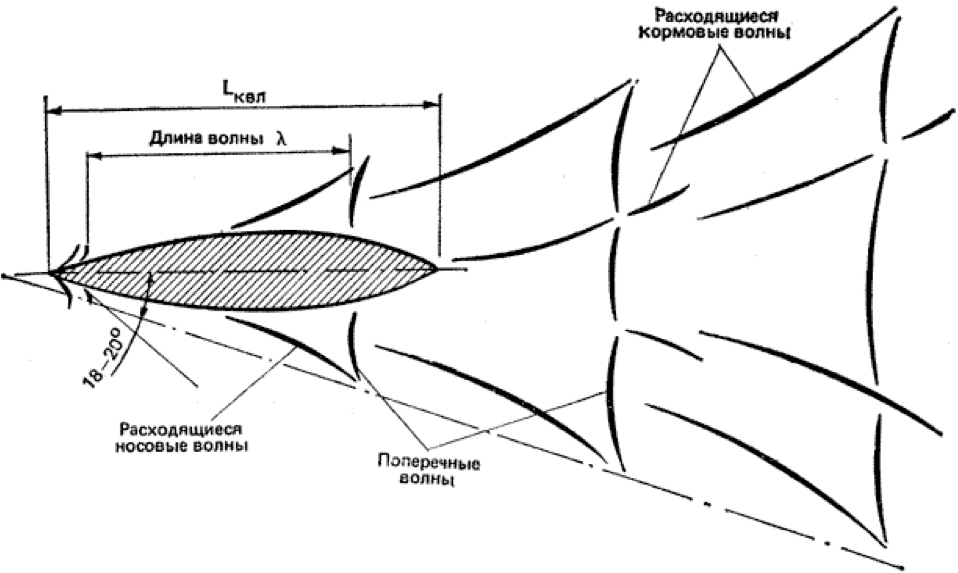
\includegraphics[scale=0.5]{0016.jpg}
  \caption{Схема волновой системы, образующейся у корпуса судна}
  \label{fig:16}
\end{figure}

Возникает сложная система носовых и кормовых волн, которая по своему характеру одинакова для судов любых размеров (рис.~\ris{16}). На малой скорости хорошо заметны расходящиеся волны, зарождающиеся в носу и корме судна. Их гребни расположены под углом 36\otdo 40\gr к диаметральной плоскости. На более высоких скоростях выделяются поперечные волны, гребни которые не выходят за пределы сектора, ограниченного углом 18\otdo 20\gr к \textit{ДП} судна. Носовая и кормовая системы поперечных волн взаимодействуют друг с другом, следствием чего может быть как увеличение высоты суммарной волны за кормой судна, так и её уменьшение. По мере удаления от судна энергия волн поглощается средой, и они постепенно затухают.

Величина волнового сопротивления изменяется в зависимости от скорости яхты. Из теории колебаний известно, что скорость распространения волн связана с их длиной $\lambda$ соотношением

\begin{equation}
  \lambda = \frac{2 \pi \cdot v^2}{\mathrm g}\,, \quad \text{м},
\end{equation}

где: $v$ \--- скорость яхты, м/с; $\mathrm g$ = 9,81 м/с$^2$ \--- ускорение силы тяжести. 

Поскольку волновая система движется вместе с яхтой, то и скорость распространения волны равна скорости яхты. Таким образом, можно подсчитать длину поперечной волны для каждой скорости яхты:

\begin{table}[htb]
  \centering
  \begin{tabular}{lcccccc}
    Скорость, уз & 2 & 4 & 6 & 8 & 10 & 12 \\
    Длина волны, м & 0,68 & 2,72 & 6,12 & 10,9 & 17 & 24,5
  \end{tabular}
  \caption{Зависимость длины поперечной волны от скорости яхты}
  \label{tab:3}
\end{table}

Если речь идет, например, о яхте длиной по ватерлинии 8 м, то при скорости 4 уз на длине корпуса разместится около трех поперечных волн, при скорости 6 уз \--- полторы. Зависимость между длиной поперечной волны $\lambda$, создаваемой корпусом длиной \lkvl движущимся со скоростью $v$, во многом определяет величину волнового сопротивления. 

Для величины сопротивления важно, какая часть носовой поперечной волны подойдет к месту, где расположен гребень кормовой волны. Если на длине яхты по \textit{КВЛ} уложится целое число полуволн, то в корме может оказаться либо вершина, либо подошва носовой поперечной волны. Произойдет соответственно неблагоприятная (рис.~\ris{17}, \textit{б}) или благоприятная (рис.~\ris{17}, \textit{а}) интерференция волн. В первом случае высота суммарной волны возрастает и, поскольку энергия волн и величина волнового сопротивления пропорциональны квадрату их амплитуд, сопротивление яхты существенно возрастает. При благоприятном сложении подошвы носов волны с вершиной кормовой суммарная высота волны снизится, сопротивление увеличится медленнее.

\begin{figure}[htb]
  \centering
  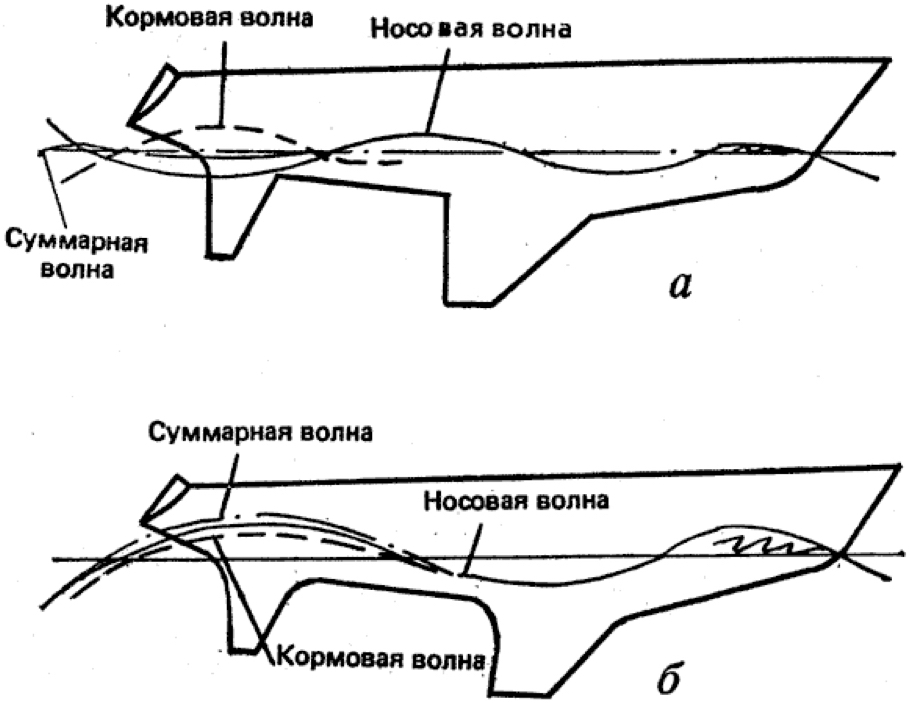
\includegraphics[scale=0.5]{0017.jpg}
  \caption{Интерференция носовой и кормовой поперечных волн}
  \label{fig:17}
  \centering
  \small
  \textit{а} \--- благоприятная;
  \textit{б} \--- неблагоприятная
\end{figure}

Многочисленными исследованиями, проведенными на моделях в опытном бассейне и на натурных судах, ycтановлено, что характер волнообразования всех судов, независимо от их размерений и абсолютной скорости, оказывается одинаков, если равны их относительные скорости или числа Фруда:

\begin{equation}
  \mathrm{Fr} = \frac{v}{(\mathrm g \cdot \lkvl)^{1/2}}
\end{equation}

Заметим, что в формулу относительной скорости входят длина судна по ватерлинии и те же символы, что и в формулу для определения длины волны в зависимости от её скорости. Этим подчеркивается взаимосвязь гравитационного характера волнообразования и его зависимость от скорости и длины судна.

На малых скоростях при $\mathrm{Fr} = 0,1\motdo 0,2$ волновое сопротивление яхты невелико. При $\mathrm{Fr} = 0,2$ на длине корпуса укладывается примерно четыре невысокие носовые поперечные волны. По мере повышения скорости волновое сопротивление начинает быстро расти. При числах Fr, равных 0,25, 0,30 и 0,50, имеет место неблагоприятная интерференция поперечных волн, а относительная скорость $\mathrm{Fr} = 0,5\motdo 0,6$ является порогом, превысить который обычная яхта водоизмещающего типа не может ни при каких обстоятельствах. На этой скорости яхта оказывается зажатой между двумя гребнями одной поперечной волны: сопротивление её возрастает пропорционально шестой степени скорости. Как правило, тяги парусов, даже при форсировании ими в свежий ветер, оказывается недостаточно, чтобы получить хотя бы небольшой прирост скорости. Поэтому скорость, соответствующую числу Фруда около 0,5, считают предельной для водоизмещающих яхт. Её можно вычислить, учитывая, что g \--- величина постоянная, по формуле\footnote{При переводе скорости из метрических мер в узлы и наоборот следует учитывать, что 1 узел = 1,852 км/ч = 0,514 м/с.}:

\begin{equation}
  v = 3 \cdot {\lkvl}^{1/2}, \quad \text{уз} 
\end{equation}

Таким образом, реальная скорость, которой могут достичь яхты отдельных типов, составляет около: 
\begin{itemize}
\item класс <<Солинг>> \--- 7,5 уз; 
\item тип <<Алькор>> \--- 9 уз; 
\item тип <<Конрад-54>> \--- 11,2 уз; 
\item класс R12 \--- 12 уз.
\end{itemize}

В ряде случаев в океанских гонках крейсерских яхт, однако, достигались более высокие скорости, которые могли развить в течение ограниченного времени суда облегченного типа. Это происходило, как правило, на попутных курсах и при крупной волне, при штормовых ветрах и форсировании парусами. В момент, когда под яхту подкатывался гребень очередной волны, смоченная поверхность корпуса резко уменьшалась и судно, выходило на режим серфинга \--- скольжения вместе с гребнем ветровой волны. При этом на яхте длиной по КВЛ 19,8 м, например, была отмечена максимальная скорость 22 уз ($v = 4,95 \cdot \lkvl$).

\begin{figure}[htb]
  \centering
  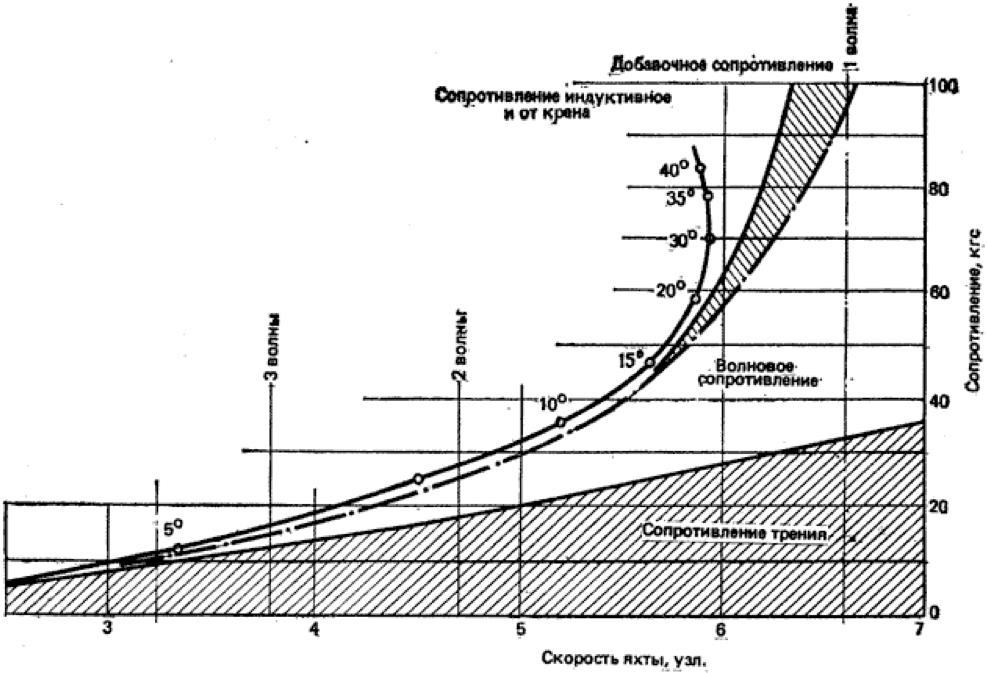
\includegraphics[scale=0.5]{0018.jpg}
  \caption{Зависимость сопротивления воды движению яхты от её скорости}
  \label{fig:18}
\end{figure}

Как видно на рис.\ris{18}, доля волнового сопротивления в общем балансе сопротивления воды движению яхты возрастает с увеличением скорости яхты. На предельных скоростях оно достигает 60\otdo 65\%, а при движении в слабый ветер на создание волн затрачивается около 30\% движущей силы парусов. Поэтому снижение волнового сопротивления особенно важно для яхт, от которых ожидают хороших результатов в свежий ветер. При разработке проекта таких яхт стараются облегчить корпус и оборудование, чтобы значение относительной длины было в пределах $\lkvl / D^{1/3} = 4,2\motdo 5,2$ (чем больше эта длина, тем меньше волновое сопротивление). Коэффициент продольной полноты $\varphi$ принимают равным 0,60, чтобы более равномерно распределить водоизмещение яхты по длине и уменьшить глубину волновой впадины вблизи миделя.

Большое влияние на волновое сопротивление оказывает и отношение $\lkvl / \bkvl$. Благодаря большому удлинению корпусов катамаранов ($\lkvl / \bkvl = 10\motdo 20$) и отсутствию на них тяжелых фальшкилей удается существенно снизить их волновое сопротивление и достичь гораздо более высоких скоростей, чем $3 \cdot {\lkvl}^{1/2}$. Например, катамаран типа <<Центаурус>> ($\lkvl = 10$\,м) при благоприятных условиях развивает скорость 18 уз ($\approx 5,8 \cdot {\lkvl}^{1/2}$). 

\textbf{Дополнительное сопротивление на взволнованном море.} Нередко яхтсмены обнаруживают, что после многих часов, затраченных на лавировку против волны, яхта выбирается на ветер считанные мили. И это после изматывающей килевой качки! 

В данном случае приходится считаться с дополнительным сопротивлением движению яхты, которое появляется вследствие килевой качки судна. Особенно заметно падение скорости яхты, если период ее собственных продольных колебаний совпадает с периодом волны, т.\=,е. при резонансе. В существовании же собственных колебаний можно убедиться, если, например, спрыгнуть с носа яхты на причал. Каждая яхта при этом ведет себя, по-разному: у одной качка порывистая скоро затухает, у другой \--- плавная продолжается долго. 

Установлено, что период собственных продольных колебаний яхты зависит от продольного момента инерции т.\=,е. от расположения масс по длине судна, от обводов корпуса, особенно в оконечностях, взаимного расположения центра тяжести площади ватерлинии и центра тяжести яхты. Если, например, \textit{ЦТ} площади ватерлинии совпадает с \textit{ЦТ} яхты. Большие массы (якоря с цепями, двигатель цистерны топлива и пресной воды и т.\=,п.) расположены далеко от миделя и обводы, носа и кормы почти симметричны, яхта имеет достаточно большой период и амплитуду собственных колебаний, который может оказаться близким к периоду наиболее неблагоприятной волны длиной от 0,8 до 1,5 длины яхты по \textit{КВЛ}. При сильной килевой качке яхта приводит в движение большие массы воды, непосредственно соприкасающиеся с корпусом, таким образом, поглощается часть энергии ветра, которая могла бы затрачиваться на продвижение судна вперед, а сопротивление воды повышается 2\otdo 25 раза (по сравнению с тихой волны). 

При проектировании яхт обычно предусматривается возможность уменьшения размахов оконечностей яхты и смягчения качки. Наиболее тяжелые массы (фальшкиль, мачту, двигатель, цистерны и т.\=,п.) стараются расположить вблизи центра тяжести судна. Обводы корпуса выше ватерлинии обычно выполняются несимметричными относительно миделя. По мере движения кормы вниз ширина ватерлинии у транца и погружающийся объем корпуса прогрессивно увеличиваются, препятствуя глубокому погружению кормы в воду и поглощая энергию качки. Хороший развал надводного борта в носу также способствует снижению ускорений носовой части яхты при движении ее вниз.
 
Большое значение для уменьшения продольной качки имеет уменьшение массы рангоута и такелажа, поскольку момент инерции массы яхты складывается из произведения отдельных масс на квадраты отстояния их от \textit{ЦТ} судна. Таким образом, влияние на продольную качку килограмма массы на топе мачты, отстоящей от \textit{ЦТ} на 12\,м, аналогично грузу 70\,кг, расположенным на уровне палубы. 

Рис.~\ris{18} дает представление о доле добавочного сопротивления при ходе на волнении для крейсерско-гоночной яхты. При увеличении скорости эта составляющая общего сопротивления может возрасти до 15\otdo 25\%, что равносильно потере скорости на 3\otdo 4\%. Потеря существенно возрастает при резонансе, поэтому экипаж должен предпринять специальные меры для уменьшения амплитуды и изменения частоты колебаний. С этой целью можно изменить курс яхты по отношению к волне, если позволяют обстоятельства, или попытаться изменить период собственных колебаний судна, переместив людей на корму. Тогда яхта получит дифферент на корму, которая своим объемом и большой шириной ватерлинии будет гасить качку. 

\textbf{Дополнительное сопротивление от крена и дрейфа.} Испытания моделей яхт в опытных бассейнах показали, что с увеличением крена сопротивление корпуса превышает сопротивление тех же моделей, испытанных на ходу без крена. В качестве примера на рис.~\ris{18} дана кривая изменения дополнительного сопротивления яхты в зависимости от угла крена и скорости. При крене до 15\gr прирост сопротивления невелик \--- не более 5\%. Однако на скорости около 6 уз и при крене 35\gr сопротивление уже на 38\% больше, чем при плавании без крена. Для рассматриваемой яхты это приводит к потере 0,4 уз скорости. 

Эксперименты позволили выяснить, что дополнительное сопротивление в данном случае может быть разделено на две составляющие \--- индуктивное сопротивление и сопротивление от крена. Обе составляющие вызваны действием кренящей силы \vidx{F}{Д} (см. рис.~\ris{4}). Основным источником индуктивного сопротивления является подъемная сила на киле и руле, перетекание воды через нижнюю кромку плавников киля и руля со стороны повышенного давления на сторону разрежения, как мы уже говорили (см. рис.~\ris{20}). Срывающиеся с нижней кромки вихри требуют дополнительных затрат энергии движущей силы. Чем больше величина подъемной силы, образующейся на плавниках, тем больше разность давлений на их сторонах и соответственно больше индуктивное сопротивление. Наоборот, с увеличением аэродинамического удлинения плавника, т.\=,е. с уменьшением средней хорды относительно площади плавника, индуктивное сопротивление уменьшается. 

Определенную долю здесь вносит и корпус яхты, который обтекается не по оптимальным ватерлиниям, а под углом дрейфа. 

Дополнительное сопротивление от крена обусловлено как появлением несимметричности в обводах корпуса, так и изменением поля гидродинамических давлений у наветренного и подветренного бортов судна. У яхт с длинными свесами крен около 5\gr вызывает иногда даже некоторое снижение полного сопротивления при увеличении смоченной длины корпуса. Широкий <<швертботный>> современный корпус при крене 8\otdo 10\gr уменьшает смоченную поверхность и сопротивление, которое может снизиться на 2\otdo 4\%. Но с увеличением крена сопротивление начинает возрастать, составляя примерно 1/3 величины дополнительного сопротивления; остальное приходится на долю индуктивного сопротивления. И все же сопротивление от крена достаточно велико \--- оно достигает около 15\% сопротивления яхты, идущей без крена. Следовательно, при участии в гонке экипаж должен принять меры к уменьшению крена.

На рис.~\ris{18} хорошо видно, что крен 30\gr является для данной яхты критическим. Дальнейшее усиление ветра, при котором судно получает дополнительный крен, приводит уже не к повышению скорости, а, наоборот, к снижению. Значит, при достижении этого крена целесообразно уменьшить площадь парусности, а на небольшой яхте попытаться откренить судно массой экипажа.

При крене не только дополнительно растет сопротивление, но и ухудшается эффективность работы парусного вооружения, увеличивается склонность яхты приводиться к ветру. Для удержания судна на курсе необходимо отклонять руль на большой угол, что дополнительно увеличивает лобовое индуктивное сопротивление руля. 

Воздушное сопротивление корпуса яхты, рубок и экипажа, расположенного на палубе, сравнительно невелико. Оно достигает заметной величины только в сильный ветер и на курсе бейдевинд. Гораздо большее, значение имеет сопротивление рангоута, парусов и такелажа, рассмотрению которых уделено внимание в гл.~\ref{chap:2}.

\chapter{Прикладная аэродинамика паруса}\label{chap:2}

\section{Работа паруса}

Современная теория паруса основывается на положениях аэродинамики крыла, элементы которой были рассмотрены в главе <<Элементы теории парусной яхты>> (см. <<Сопротивление дрейфу>>). Механика возникновения аэродинамической силы на парусе, изготовленном из ткани, в принципе аналогична и для жесткого профилированного крыла. В любом поперечном сечении паруса должна развиться циркуляция потока воздуха, как вокруг профиля крыла (см. рис.~\ris{8}), чтобы появилась подъемная сила.

Естественно, что аэродинамика паруса из ткани имеет ряд существенных отличий от жесткого крыла, каким, например, является яхтенный киль. Вследствие эластичности ткани парус изменяет свой профиль под влиянием потока воздуха. Он обладает способностью скручиваться \--- изменять угол атаки по отношению к ветру по высоте. В отличие от получивших распространение аэродинамических профилей со сравнительно толстой входящей кромкой парус имеет острую переднюю кромку и выпукло\-/вогнутую форму, образованную тонким материалом. Наконец, передней кромкой парус может крепиться к мачте, имеющей довольно большое поперечное сечение, что вносит существенное изменение в картину обтекания паруса потоком и в распределении давления по ширине паруса.

\begin{figure}[htb]
  \centering
  \includegraphics{0019}
  \caption{Схема сил, действующих на паруса яхты; основные угловые параметры движения и установки парусов}
  \label{fig:19}
  \centering{}
  \small
  $\beta$ \--- путь яхты по отношению к вымпельному ветру; $\lambda$ \--- угол дрейфа; $\alpha$ \--- угол атаки паруса; $\delta$ \--- угол установки паруса относительно \textit{ДП} яхты; \vidx{V}{И} \--- скорость истинного ветра; \ve V \--- скорость яхты; \vidx{V}{В} \--- скорость вымпельного ветра; \vidx{V}{НА} \--- скорость прямо против ветра (???)
\end{figure}

Наиболее важные элементы, влияющие на аэродинамику паруса, будут рассмотрены дальше, но для начала установим влияние составляющих аэродинамической силы на движение яхты при различных курсах относительно ветра.

Если яхта идет курсом бейдевинд, то под действием набегающего потока воздуха на парусах, установленных под углом атаки $\alpha$ к направлению вымпельного ветра, возникает результирующая аэродинамическая сила \ve A (рис.~\ris{19}). По аналогии с жестким крылом эту силу можно разложить на две составляющие: подъемную силу \ve Y, перпендикулярную направлению вымпельного ветра, и лобовое сопротивление \ve X, действующее по направлению ветра. В дальнейшем эти силы мы будем использовать для рассмотрения характеристик паруса и всего парусного вооружения в целом. 

Для того чтобы оценить влияние аэродинамической силы \ve A на движение яхты, представим ее в виде двух других составляющих: силы тяги \ve T, направленной по оси движения судна, и перпендикулярной ей силы дрейфа \ve D. Направление движения яхты (путь) отличается от ее курса на величину угла дрейфа $\lambda$, однако в дальнейшем анализе этим углом можно пренебречь. 

Предположим, что на выбранном курсе бейдевинд удалось увеличить подъемную силу на парусе до величины \vidx{Y}{1}, а лобовое сопротивление не изменилось. Силы \vidx{Y}{1} и \ve X, будучи сложенными по правилу сложения векторов, образуют новую аэродинамическую силу \vidx{A}{1}. Изменятся и ее составляющие относительно оси движения яхты \ve T и \ve D. Без вычислений можно сказать, что в данном случае с увеличением подъемной силы увеличатся и сила тяги, и сила дрейфа (рис.~\ris{20}). Аналогичное построение позволяет убедиться, что при увеличении лобового сопротивления на курсе бейдевинд сила тяги уменьшается, а сила дрейфа увеличивается. Таким образом, при плавании в лавировку экипаж яхты должен стремиться по возможности добиться образования на парусах максимальной подъемной силы при минимальной величине лобового сопротивления. Иными словами, для острых курсов необходима работа паруса с максимальным аэродинамическим качеством, которое численно выражается в отношении подъемной силы к лобовому сопротивлению. 

\begin{equation}
\ve K = \ve Y / \ve X
\end{equation}

Отметим, что на курсе бейдевинд вымпельный ветер, являющийся результатом сложения векторов истинного ветра и движения яхты, имеет наивысшую скорость \vidx{V}{В} (см. рис.~\ris{19}, \textit{б}), что сказывается на величине обеих составляющих аэродинамической силы \--- \ve Y и \ve X.

На курсе галфвинд подъемная сила является силой тяги, а лобовое сопротивление \--- силой дрейфа. Если лобовое сопротивление увеличить, то увеличится только сила дрейфа. Однако на ходовые качества яхты это влияет в заметно меньшей степени, чем на курсе бейдевинд, поскольку скорость вымпельного ветра на курсе галфвинд снизилась и, следовательно, величина силы дрейфа меньше.

\begin{figure}[htb]
  \centering
  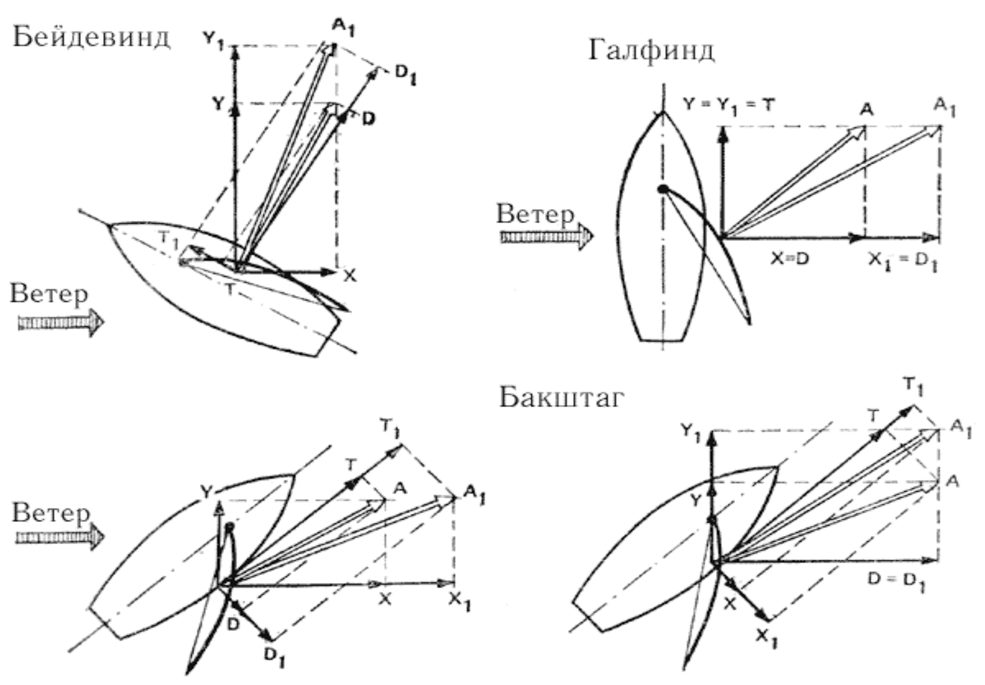
\includegraphics[scale=1]{0020}
  \caption{Роль составляющих аэродинамической силы на различных курсах относительно вымпельного ветра}
  \label{fig:20}
\end{figure}

На курсе бакштаг парус работает на больших углах атаки, при которых подъемная сила оказывается значительно меньше лобового сопротивления. Если увеличить лобовое сопротивление, то тяга и сила дрейфа увеличатся. При возрастании подъемной силы тяга также увеличивается, а сила дрейфа уменьшается. Следовательно, на курсе бакштаг рост и подъемной силы и (или) лобового сопротивления увеличивает тягу. Сила дрейфа тем больше, чем больше лобовое сопротивление. На курсе фордевинд угол атаки паруса близок к 90\gr, поэтому подъемная сила на парусе равна нулю, а лобовое сопротивление направлено по оси движения яхты и становится силой тяги. Сила дрейфа равна нулю. Следовательно, на курсе фордевинд для увеличения силы тяги нужно увеличивать лобовое сопротивление парусного вооружения, что на гоночных яхтах достигается постановкой дополнительных парусов \--- \textbf{спинакера} и \textbf{блупера}, имеющих большую площадь и плохо обтекаемую форму. 

Отметим, что на курсе фордевинд на паруса действует вымпельный ветер минимальной скорости, в результате чего на паруса действуют сравнительно умеренные силы.

\section{Особенности работы паруса как крыла}

Только при небольшом значении угла атаки, когда на остром и тонком профиле еще не образуется подъемная сила, парус обтекается потоком воздуха, одинаково плавным с нижней и с верхней стороны. При небольшом увеличении угла атаки критическая точка перемещается на нижнюю сторону профиля и потоку приходится огибать острую кромку с большой скоростью. В результате у входящей кромки образуется значительное разрежение и под влиянием этого разрежения пограничный слой отрывается от поверхности профиля, образуя на его спинке вихревой пузырь. При достаточно большой скорости ветра поток быстро поглощает энергию вихрей и слой вновь  присоединяется к поверхности профиля на некотором расстоянии от входящей кромки (рис.~\ris{21}).

\begin{figure}[htb]
  \centering
  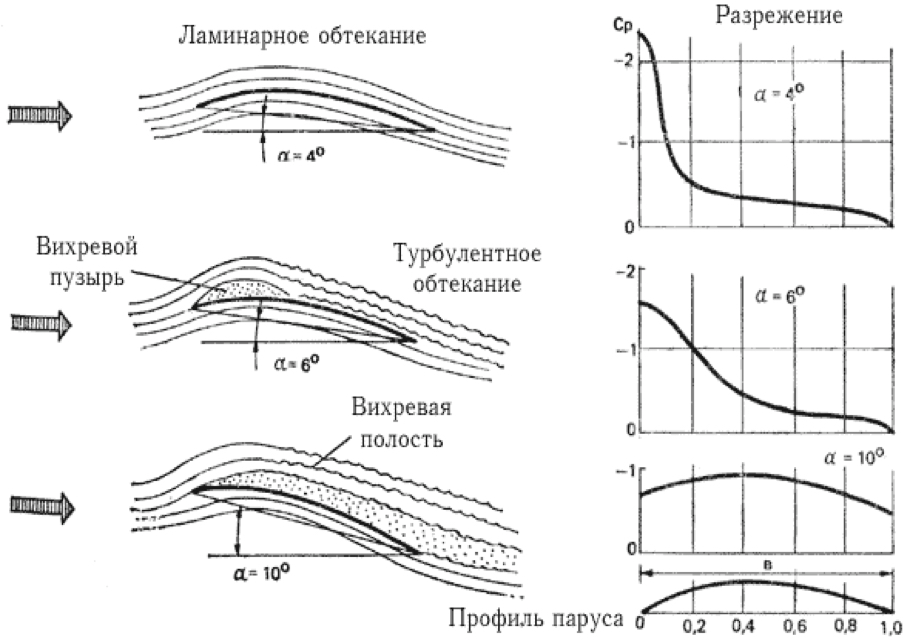
\includegraphics[scale=1]{0021}
  \caption{Результаты замеров разрежения на жестком выпукло-вогнутом профиле}
  \label{fig:21}
\end{figure}

Вихревой пузырь, размеры которого увеличиваются по мере увеличения угла атаки, вносит существенные изменения в распределение пониженного давления вдоль подветренной стороны паруса по сравнению с показанным на рис.~\ris{10} распределением давления на жестком профиле с толстой скругленной передней кромкой. Напомним, что именно разрежение на подветренной стороне паруса играет основную роль в создании подъемной силы и, следовательно, силы тяги на острых к ветру курсах. 

На рис.~\ris{21} представлены результаты замеров разрежения на жестком выпукло-вогнутом профиле, аналогично парусу. На малых углах атаки профиль обтекается плавным ламинарным потоком. 

При $\alpha = 4\gr$ начинаете отрыв пограничного слоя. В этот момент достигается наивысшее разрежение, пик которого расположен вблизи входящей кромки.
 
При $\alpha = 6\gr$ вихревой пузырь занимает на подветренной стороне около 25\% хорды профиля $b$. Разрежение уменьшается, и эпюра его становится более плавной. 

При $\alpha = 10\gr$ пузырь охватывает всю ширину профиля, его толщина составляет 3,5\% $b$. Давление повышается в 2,5 раза по сравнению с разрежением при $\alpha = 4\gr$; пика разрежения практически нет \--- оно равномерно распределено по всей ширине профиля. Значит, подъемная сила существенно снизилась, а лобовое сопротивление возросло (см. рис.~\ris{27}). 

Таким образом, на курсе бейдевинд увеличение угла атаки паруса к вымпельному ветру более 5\otdo 6\gr нежелательно. На реальном парусе вихревой пузырь представляет собой невидимый глазу цилиндрический валик, распространяющийся по всей высоте паруса. Чем больше выбран шкот, тем большая часть подветренной поверхности паруса захватывается вихревым валиком, уменьшая подъемную силу. 

Для выбора оптимального угла атаки в последние годы используются индикаторы обтекания в виде ленточек из тонкой ткани, закрепленных на определенном расстоянии от передней шкаторины с обеих сторон паруса (рис.~\ris{22}).

\begin{figure}[htb]
  \centering
  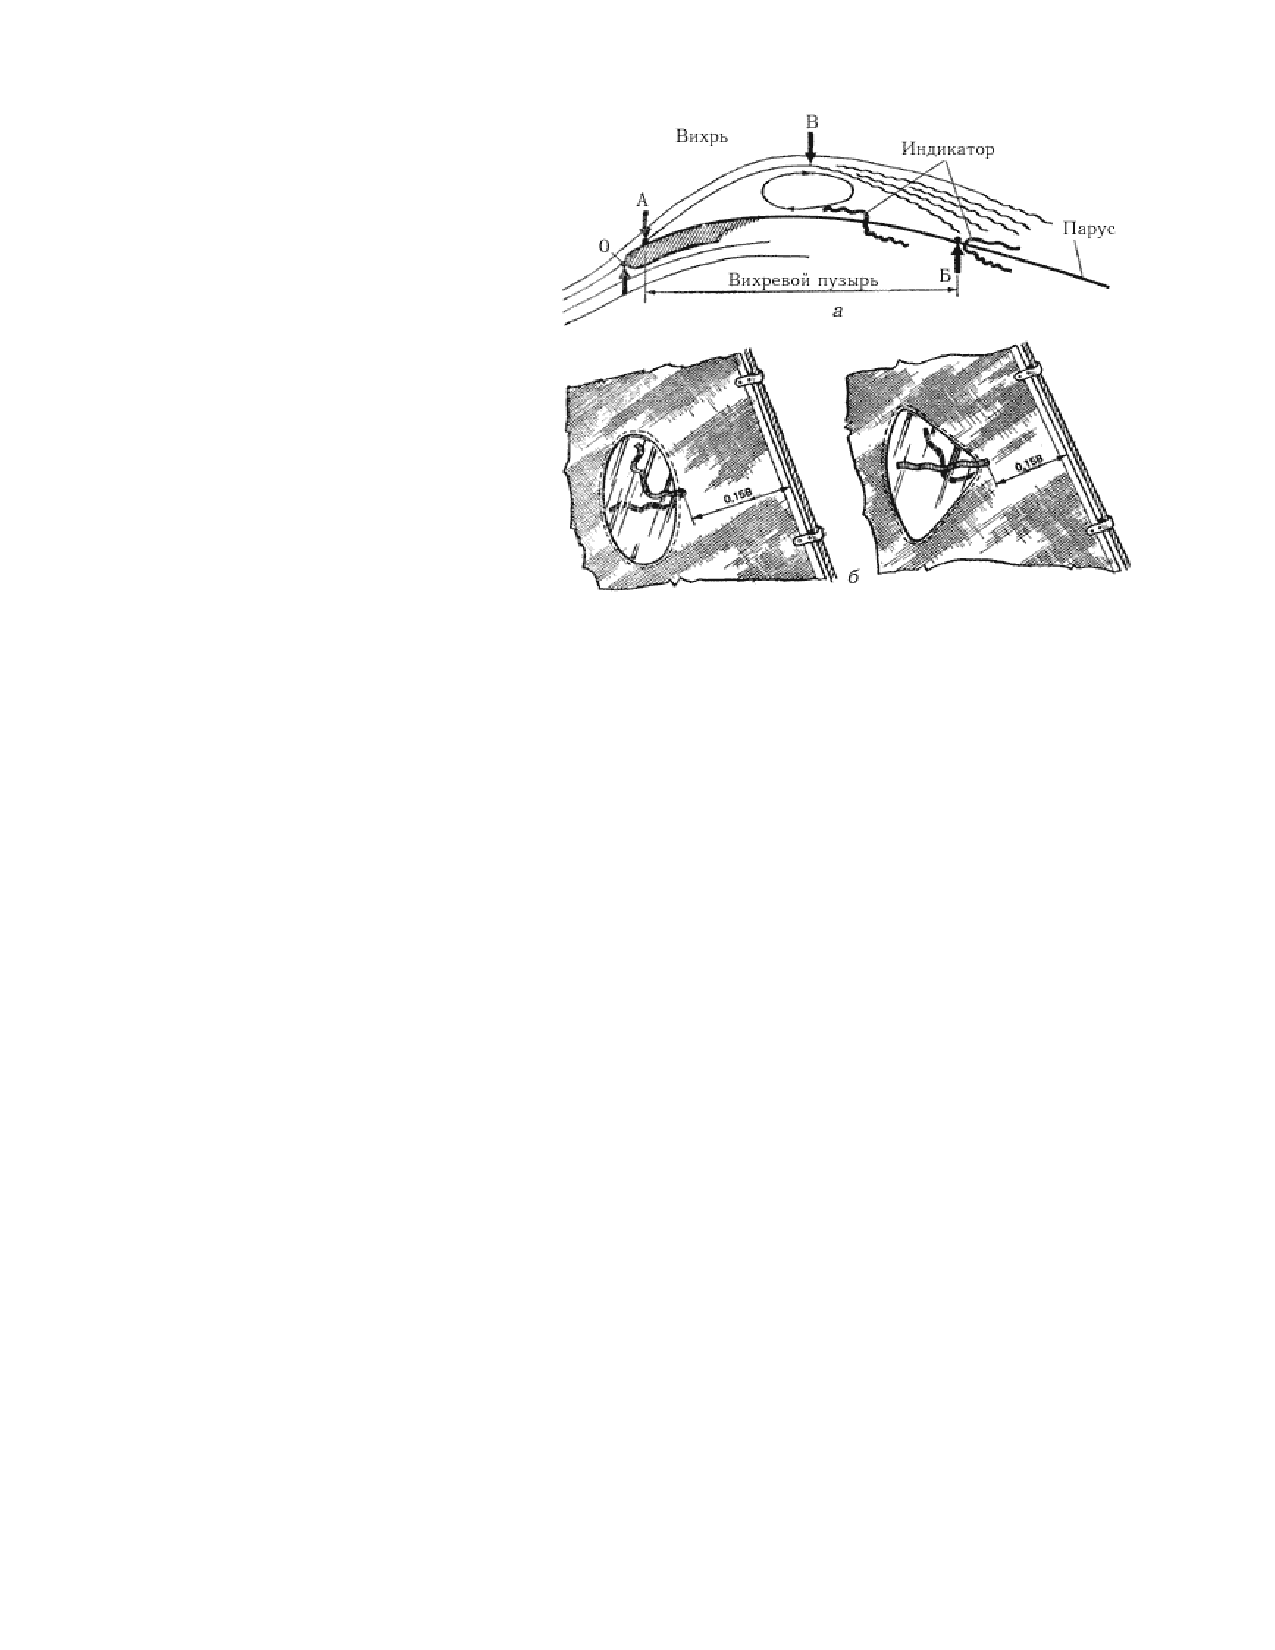
\includegraphics[scale=1]{0022}
  \caption{Индикаторы обтекания на парусе}
  \label{fig:22}
\end{figure}

Таким местом является точка Б возвpaтa пограничного слоя к поверхности паруса. При угле атаки $\alpha = 5\gr$ она отстоит от передней шкаторины примерно на 15\% ширины паруса в каждом его поперечном сечении. Как только вихревой пузырь достигнет этой точки, ленточка индикатора на подветренной поверхности паруса, ранее направленная назад по потоку воздуха, отклонится вверх и вперед, указывая на возникновение здесь вихрей. Дальнейшее выбирание шкотов \--- увеличение угла атаки \--- не только бесполезно, но даже вредно, так как приводит к большой потере подъемной силы.

Установка трех\-/четырех подобных индикаторов, равномерно распределенных по высоте стакселя, облегчает рулевому правильный выбор курса при лавировке. Выбрав наивыгоднейшим образом шкоты для данного курса, ведут яхту таким образом, чтобы индикаторы на наветренной стороне стакселя слегка подрагивали, а на подветренной были вытянуты в сторону задней шкаторины (рис.~\ris{23}).
 
Причиной падения подъемной силы на парусе является срыв потока с его подветренной стороны при увеличении угла атаки (что соответствует подбиранию шкотов или уваливанию яхты), поэтому главную роль играют индикаторы, расположенные на подветренной стороне. Если они начинают подниматься и совершать беспорядочные движения, значит, необходимо привести яхту к ветру или потравить шкоты.

Угол атаки, при котором подъемная сила перестает расти, называется критическим углом атаки. Его величина зависит от глубины и формы <<пуза>> паруса, аэродинамического удлинения $\lambda$ (оно для парусов вычисляется так же, как и для килей и рулей), наличия у передней шкаторины мачты или обтекателя штага.

\begin{figure}[htb]
  \centering
  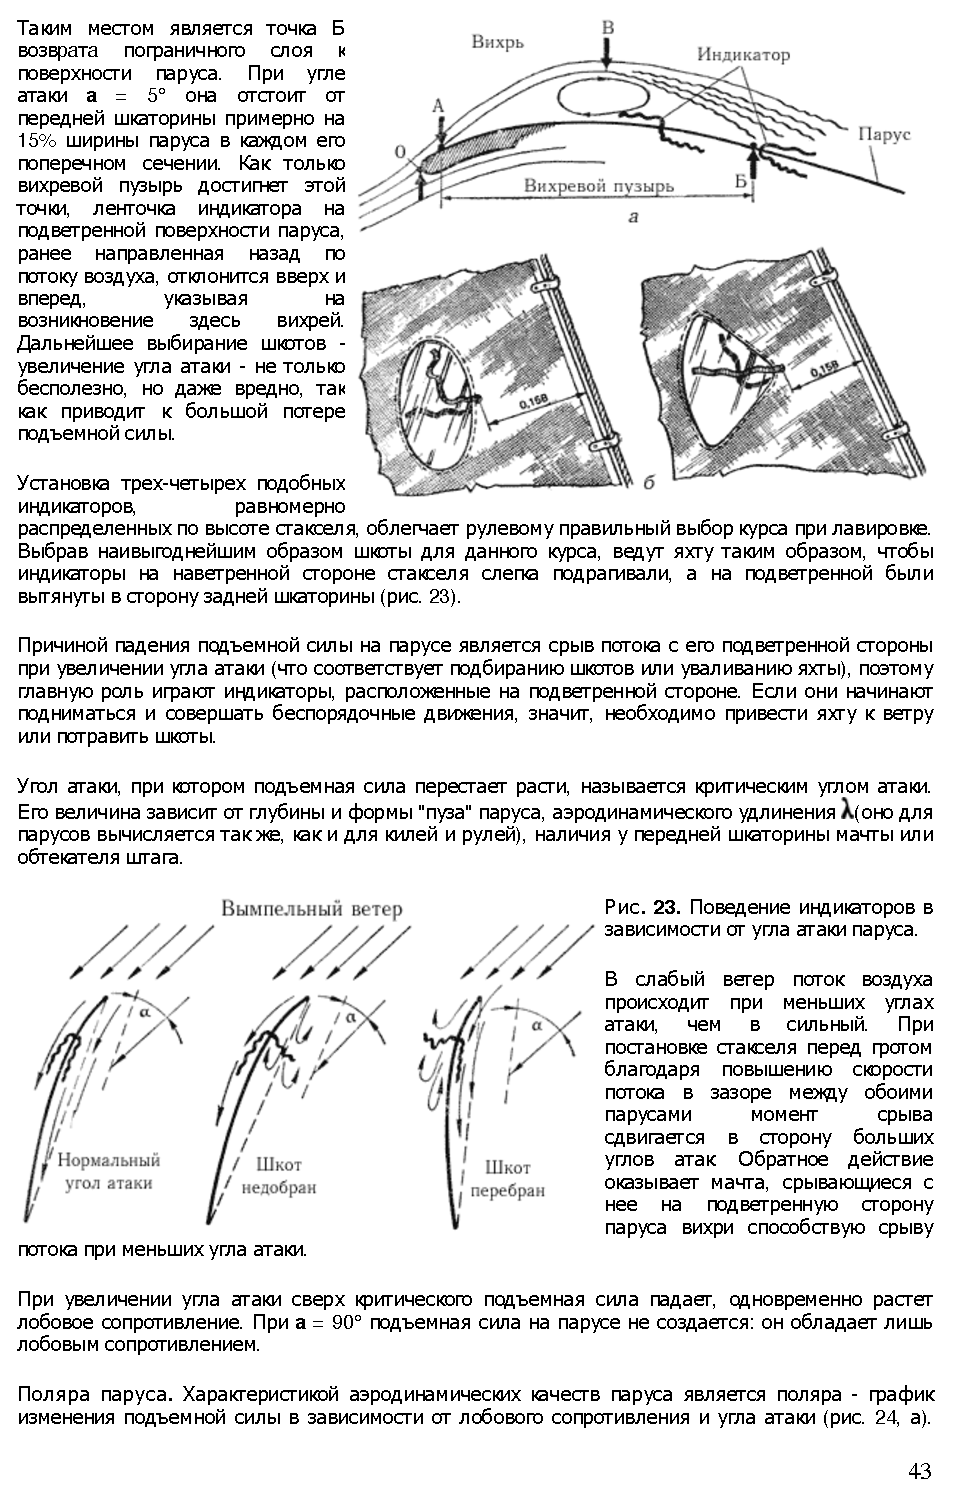
\includegraphics[scale=1]{0023}
  \caption{Поведение индикаторов в зависимости от угла атаки паруса}
  \label{fig:23}
\end{figure}

В слабый ветер поток воздуха происходит при меньших углах атаки, чем в сильный. При постановке стакселя перед гротом благодаря повышению скорости потока в зазоре между обоими парусами момент срыва сдвигается в сторону больших углов атак. Обратное действие оказывает мачта, срывающиеся с нее на подветренную сторону паруса вихри способствую срыву потока при меньших угла атаки. 

При увеличении угла атаки сверх критического подъемная сила падает, одновременно растет лобовое сопротивление. При $\alpha = 90\gr$ подъемная сила на парусе не создается: он обладает лишь лобовым сопротивлением.

\textbf{Поляра паруса.} Характеристикой аэродинамических качеств паруса является поляра \--- график изменения подъемной силы в зависимости от лобового сопротивления и угла атаки (рис.~\ris{24}, \textit{а}). Для того чтобы поляру можно было применить к парусу любых размеров, по осям координат откладывают не значения сил, а безразмерные коэффициенты подъемной силы \cidx{C}{Y} и лобового сопротивления \cidx{C}{X}. Данные для построения поляры получают в результате продувок моделей парусов в аэродинамических трубах. 

\begin{figure}[htb]
  \centering
  \includegraphics[scale=1]{0024}
  \caption{Поляра паруса}
  \label{fig:24}
\end{figure}

С помощью поляры можно определить величины подъемной силы и лобового сопротивления, а также их составляющих \--- проекций на направление движения яхты. Опустив, например, из точки поляры, соответствующей углу атаки $\alpha = 20\gr$, перпендикуляр на ось движения яхты, можно найти величину коэффициента силы тяги \cidx{C}{Т} как отрезка прямой \cidx{А}{О}. Длина самого перпендикуляра $AB$ будет не что иное, как коэффициент силы дрейфа \cidx{C}{d}. Умножив численные значения коэффициентов \cidx{C}{Т} и \cidx{С}{d} на площадь паруса $S$ и скоростной напор $(\rho v^2)/2$, можно получить величину соответствующих сил. 

Поляра паруса позволяет определить наивыгоднейший угол установки парусов на данном курсе по отношению к ветру. Максимальная тяга, очевидно, определяется перпендикуляром к оси движения яхты, который одновременно является касательной к поляре. Угол атаки $\alpha = 14\gr$, определяемый точкой касания $C$, будет в данном случае наивыгоднейшим. Соответствующий ему угол установки паруса относительно \textit{ДП} яхты $\delta$ несложно найти, вычтя из курсового угла (по отношению к вымпельному ветру $\beta$ дрейф $\lambda$) и угол атаки $\alpha$ (см. рис.~\ris{19}).

Несложно выполнить аналогичные построения для различных значений курсового угла $\beta$ и определить наивыгоднейшие углы установки паруса и соответствующие им углы атаки. Можно убедиться, что для данного паруса почти на всех острых углах к ветру, вплоть до бакштага, наивыгоднейшие углы атаки близки и находятся в пределах 14\otdo 15\gr.

\textbf{Скручивание паруса.} С выбором оптимального угла атаки паруса связано его свойство скручиваться, т.\=,е. изменять угол атаки по высоте. При выбирании шкотов удается контролировать только нижнюю треть паруса; в верхней же части ткань имеет возможность несколько отклоняться на подветер, уменьшая тем самым угол атаки. Если не предусмотреть специальных средств для контроля скручивания паруса, то разность в углах атаки или угол скручивания может достичь 20\gr. А так как парус выбирают, ориентируясь на поведение его верхней части (пока не перестанет заполаскивать ткань у передней шкаторины), то нижняя часть оказывается работающей с избыточными углами атаки. Здесь может произойти срыв потока с подветренной стороны и соответственно упасть подъемная сила. Следовательно, тяга скрученного паруса оказывается ниже, чем если бы каждое его сечение по высоте имело оптимальный угол атаки. 

Особенно сильно заметно скручивание паруса на полных курсах и при свежем ветре, когда шкоты потравлены и нок гика задирается вверх. При этом верхняя часть паруса уходит под ветер и почти заполаскивает, а нижняя работает под слишком большим углом атаки. 

Для уменьшения скручивания грота на большинстве яхт применяют оттяжки гика, препятствующие задиранию нока вверх, а также проводку гика\-/шкота с одним или двумя поперечными погонами, простирающимися на всю ширину яхты. При мещении ползуна гика\-/шкота к борту яхты тяга шкотов становится почти вертикальной, благодаря чему удается держать заднюю шкаторину паруса на острых курсах более тугой. 

Свидетельством правильной регулировки натяжения оттяжки гика может служить одновременное (по всей высоте) заполаскивание ткани у передней шкаторины при потравливании шкота.

Было бы ошибкой считать, что парус вообще не должен иметь скручивания по высоте, т. е. иметь все сечения повернутыми относительно гика на один и тот же угол. На крупных яхтах надо учитывать изменение скорости и направления вымпельного ветра по высоте и наличие в верхней части паруса перетекания воздуха из зоны повышенного давления на подветренную сторону. В зависимости от высоты парусности и скорости ветра получается разность в углах атаки от 3\otdo 5\gr в бейдевинд до 10\otdo 12\gr на курсе бакштаг. В таких пределах скручивание паруса допустимо и способствует более эффективной его работе. 

Циркуляция воздуха вокруг крыла (см. рис.~\ris{10}), появляющаяся вместе с аэродинамической силой, вызывает незначительные по скорости поперечные потоки воздуха \cidx{V}{И} у входящей и выходящей кромок. Вследствие перетекания воздуха через кромки у концов крыла эти потоки усиливаются и отклоняют основной поток, набегающий на крыло, так, что угол атаки жесткого треугольного бермудского паруса по мере приближения к вершине увеличивается и близ фалового угла примерно на 20\% превышает угол атаки средней части паруса. Близ гика фактический угол атаки, наоборот, несколько уменьшается.

Таким образом, если бы парус не имел скручивания, то его верхняя часть работала бы при закритических углах атаки и практически не участвовала бы в создании движущей силы. Опытный экипаж постоянно контролирует и регулирует скручивание паруса в зависимости от силы ветра и курса яхты с помощью оттяжки гика и перемещения нижнего блока гика\-/шкота по погону.

\textbf{Влияние мачты.} Мачта является источником образования завихрений, которые особенно неблагоприятно сказываются на формировании потока на подветренной стороне паруса. Здесь вихревой след мачты уменьшает разрежение, вследствие чего уменьшается величина подъемной силы. Кроме того, сама мачта обладает достаточно большим лобовым сопротивлением. 

\begin{figure}[htb]
  \centering
  \includegraphics[scale=1]{0025}
  \caption{Влияние мачты}
  \label{fig:25}
\end{figure}

Большую роль играет форма поперечного сечения мачты, особенно передней ее кромки, на которой формируется поток. Важно, чтобы на курсе бейдевинд, когда яхта идет под углом 25\otdo 30\gr к вымпельному ветру, вихревая дорожка, срывающаяся с подветренной стороны мачты, имела бы минимальную ширину. Парус за мачтой параболическим поперечным сечение и тупой кормовой кромкой обладает более высоким аэродинамическим качеством, чем за мачтой эллиптического сечения (рис.~\ris{25}). Наиболее оптимальным оказывается вариант мачты с парусом, закрепленным передней шкаториной близ ее подветренной стороны: качество его работы на 40\% выше, чем паруса с эллиптической мачтой. Это лишнее свидетельство тому, что отрицательное влияние мачты в основном распространяется на подветренную сторону паруса.

Мачта, имеющая большое поперечное сечение, может снизить подъемную силу паруса на 25\% по сравнению с парусом, поставленным на штаге. Особенно велики потери подъемной силы при постановке паруса на рельсе с ползунками, когда в щель между мачтой и парусом перетекает воздух с наветренной стороны паруса в область пика разрежения на подветренной стороне. Неудачны мачты цилиндрического сечения, без сужения к топу: в верхней части отношение диаметра мачты уменьшающейся здесь ширине пару становится велико. Может оказаться, что часть паруса близ фалового yгла вообще не будет участвовать в создании подъемной силы, а следовательно, и тяги на курсе бейдевинд.

Наибольшее распространение на яхтах получили мачты, имеющие овальное поперечное сечение, с соотношением около 3:2, обеспечивающее большую продольную жесткость. Каплевидные и другие типы обтекаемых профилей целесообразны только в том случае, если мачта вращается для установки под наивыгоднейшим углом к вымпельному ветру при перемене галса. Такими мачтами снабжают обычно буepa и катамараны.

\section{Форма паруса и контроль за нею}

\begin{figure}[htb]
  \centering
  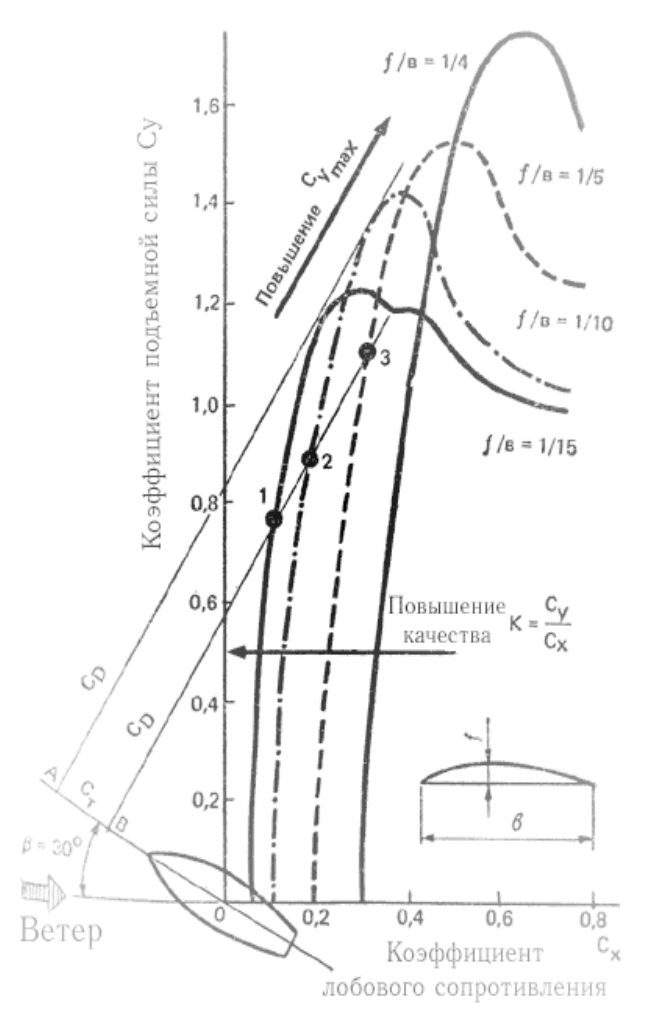
\includegraphics[scale=1]{0026}
  \caption{Поляры четырех жестких моделей бермудских парусов}
  \label{fig:26}
\end{figure}

\textbf{Поперечный профиль паруса.} Основным фактором, влияющим на величину аэродинамических сил на парусе и его тяговые характеристики, является его профиль, т.\=,е. форма и размеры <<пуза>>.

На рис.~\ris{26} представлены поляры четырех жестких моделей бермудских парусов, имеющих аэродинамическое удлинение $\lambda = 4$ и расстояние максимальной глубины <<пуза>> от передней шкаторины, равное 1/3 хорды. От реальных парусов модели отличались еще отсутствием угла скручивания и постоянством относительной глубины <<пуза>> по высоте.

На полярах (рис.~\ris{26}) видно, что с уменьшением глубины <<пуза>> качество паруса возрастает благодаря снижению коэффициента лобового сопротивления (показано горизонтальной стрелкой). Максимальная подъемная сила паруса, наоборот, увеличивается по мере увеличения глубины <<пуза>> (показано наклонной стрелкой).

Посмотрим теперь, каким образом могут быть реализованы качества парусов в зависимости от их профиля. Предположим, что яхта идет курсом бейдевинд под углом $\beta = 30\gr$ к направлению вымпельного ветра. Очевидно, наибольшую тягу даст тот парус, касательная к поляре которого \--- перпендикуляр к линии пути яхты (см. рис.~\ris{24}) будет отстоять от точки 0 дальше подобных же касательных к другим полярам. В данном случае наибольшую тягу имеет парус с относительной глубиной <<пуза>> $f/b=1/10$. Однако нетрудно заметить, что выигрыш в тяге этого паруса будет минимальным по сравнению с более плоским парусом, имеющим $f/b = 1/15$. В то же время, более <<пузатый>> парус ($f/b = 1/10$) дает значительно большую поперечную силу дрейфа, чем парус с $f/b = 1/15$. Поэтому небольшое преимущество более <<пузатого>> паруса может быть реализовано на лавировке только в слабый ветер, когда абсолютная величина силы дрейфа будет невелика. В свежий ветер плавание с таким парусом сопровождается большим креном и соответственно дополнительным сопротивлением движению, так что в конечном счете выигрыша в скорости не получится. 

Еще более <<пузатые>> паруса $f/b=1/5$ и $f/b=1/4$ на курсе бейдевинд не только не дают увеличения силы тяги, но и отличаются намного большей величиной силы дрейфа. Однако более высокий коэффициент подъемной силы <<пузатых>> парусов может быть реализован на других, более полных, курсах по отношению к ветру: например, на курсе галфвинд, когда подъемная сила дает наибольшую составляющую на направление движения (см. рис.~\ris{24}, \textit{б}). В практике морских гонок это качество <<пузатых>> парусов используется благодаря смене на полных курсах лавировочных передних парусов на дрифтергеную, блупер или спинакер.

Следует заметить, что преимущества <<пузатых>> парусов могут быть использованы в основном при слабых ветрах, когда скорость яхты прямо пропорциональна силе тяги. В сильные ветра, когда яхта развивает свою предельную скорость под обычными лавировочными парусами и дальнейшее повышение тяги практически не увеличивает скорость, постановка <<пузатых>> парусов не дает эффекта. Более того, большая сила дрейфа <<пузатого>> паруса обусловливает больший крен и дрейф и соответствующее повышение сопротивления воды движению яхты. 

В качестве основных (лавировочных) парусов для среднего ветра (2\otdo 4 балла) применяют паруса с <<пузом>> $f/b=9\motdo 10\%$. Для слабого ветра выгодны более <<пузатые>> паруса \--- $f/b$ до 12\%, а при ветре более 5 баллов \--- паруса с <<пузом>> не более 6\% ($f/b=1/17\motdo 1/25$). 

В гонках яхтсмены широко пользуются различными способами регулирования величины <<пуза>> парусов в зависимости от силы ветра. Особенно это относится к настройке грота, так как по правилам IOR замена его во время гонок не допускается, а ветровые условия могут изменяться в довольно широких пределах. Основными средствами регулирования <<пуза>> грота являются продольный изгиб мачты, натяжение шкаторин (оттяжка Кэнингхэма и грота\-/шкот), уплощающий риф, натяжение гика\-/шкота и положение его блока на погоне по ширине яхты, оттяжка гика. Продольный изгиб мачты позволяет контролировать две верхние трети паруса, в то время как другие средства эффективны при изменении профиля у гика.

В слабый ветер, когда важно иметь грот наиболее <<пузатым>>, мачта должна быть прямой, грота\-/шкот и оттяжку гика выбирают не до конца, оттяжка Кэнингхэма растравлена. Блок на погоне гика\-/шкота перемещают от \textit{ДП} в сторону наветренного борта; гика\-/шкот втугую не выбирают.

Для увеличения <<пуза>> стакселя или генуи блок (кипу) стаксель\-/шкота перемещают вперед и ближе к \textit{ДП} яхты. При этом <<пузо>> перемещается вперед, натяжение задней шкаторины ослабляется, зазор между гротом и стакселем увеличивается. 

С усилением ветра мачте придают изгиб с выпуклостью, направленной вперед, увеличивая натяжение ахтерштага (при оснастке типа 3/4 или 7/8) или регулируя натяжение промежуточного штага и бакштагов (при топовой оснастке). Благодаря этому излишек паруса убирается в образовавшийся серп у передней шкаторины, <<пузо>> становится меньше и перемещается ближе к мачте. Оттяжку Кэнингхэма, грота\-/шкот и оттяжку гика выбираю втугую; блок гика\-/шкота смещают по погону на подветренный борт. Шкоты выбирают более туго, чем в слабый ветер. При необходимости сделать парус еще более плоским в нижней части берут уплощающий риф, используя люверсы, расположенные вблизи гика.

Профиль генуи может быть сделан более плоским при передвижении блока стаксель\-/шкота назад и к борту большем натяжении передней шкаторины. Значительное влияние на профиль передних парусов оказывает натяжение штага: для того чтобы парус стал более плоским, необходимо по возможности ликвидировать прогиб штага.

Большое влияние на тяговые характеристики паруса кроме величины <<пуза>> оказывает место положения максимальной выпуклости от передней шкаторины. На рис.~\ris{27} показано распределение разрежения на подветренной стороне жесткой модели паруса с относительной величиной <<пуза>> $f/b = 0,188$ при отстоянии максимального <<пуза>> на 40 и 60\% хорды от передней кромки и при угле атаки $\alpha = 15\gr$ (характерный <<провал>> на эпюре давления являйся следствием развитого вихревого пузыря \--- см. рис.~\ris{21}). Как видим, в создании движущей силы главную роль играет передняя часть паруса, где концентрируется разрежение у паруса с <<пузом>>, расположенным на 40\% хорды от передней шкаторины. Когда же <<пузо>> смещено к задней шкаторине, область разрежения охватывает и заднюю часть профиля, вследствие чего увеличивается составляющая \ve R, направленная против движения яхты. Таким образом, при смещении <<пуза>> к задней шкаторине эффективность паруса снижается как в результате падения подъемной силы в передней части паруса, так и в результате роста сил сопротивления, тормозящих ход судна.

\begin{figure}[htb]
  \centering
  \includegraphics[scale=1]{0027}
  \caption{Распределение разрежения на подветренной стороне жесткой модели паруса}
  \label{fig:27}
\end{figure}

Лавировочные паруса шьют с максимальной глубиной <<пуза>>, расположенной от передней шкаторины на расстоянии от 35\otdo 40\% ширины паруса $b$ для плоских парусов, до 40\otdo 50\% $b$ для более полных.

Во всех поперечных сечениях максимальная глубина <<пуза>> должна находиться в указанных пределах. Поэтому по мере увеличения ширины паруса по направлению к гику соответственно увеличивается и абсолютная величина <<пуза>>. У гика на обезветренном парусе <<пузо>> образует <<мешочек>>, который в сильный ветер можно убрать в скатку уплощающего рифа.

\textbf{Форма паруса.} С точки зрения аэродинамики крыла наиболее выгодным был бы парус с эллипсовидной верхней частью. Именно в его верхней части образуются потоки воздуха, перетекающего с наветренной стороны на подветренную \--- в область разрежения. В результате возникают вихри, срывающиеся с кромки паруса и уходящие в пространство. Эти возмущения требуют затрат кинетической энергии ветра, которые выражаются в росте общего аэродинамического сопротивления судна в виде составляющей индуктивного сопротивления. 

\begin{figure}[htb]
  \centering
  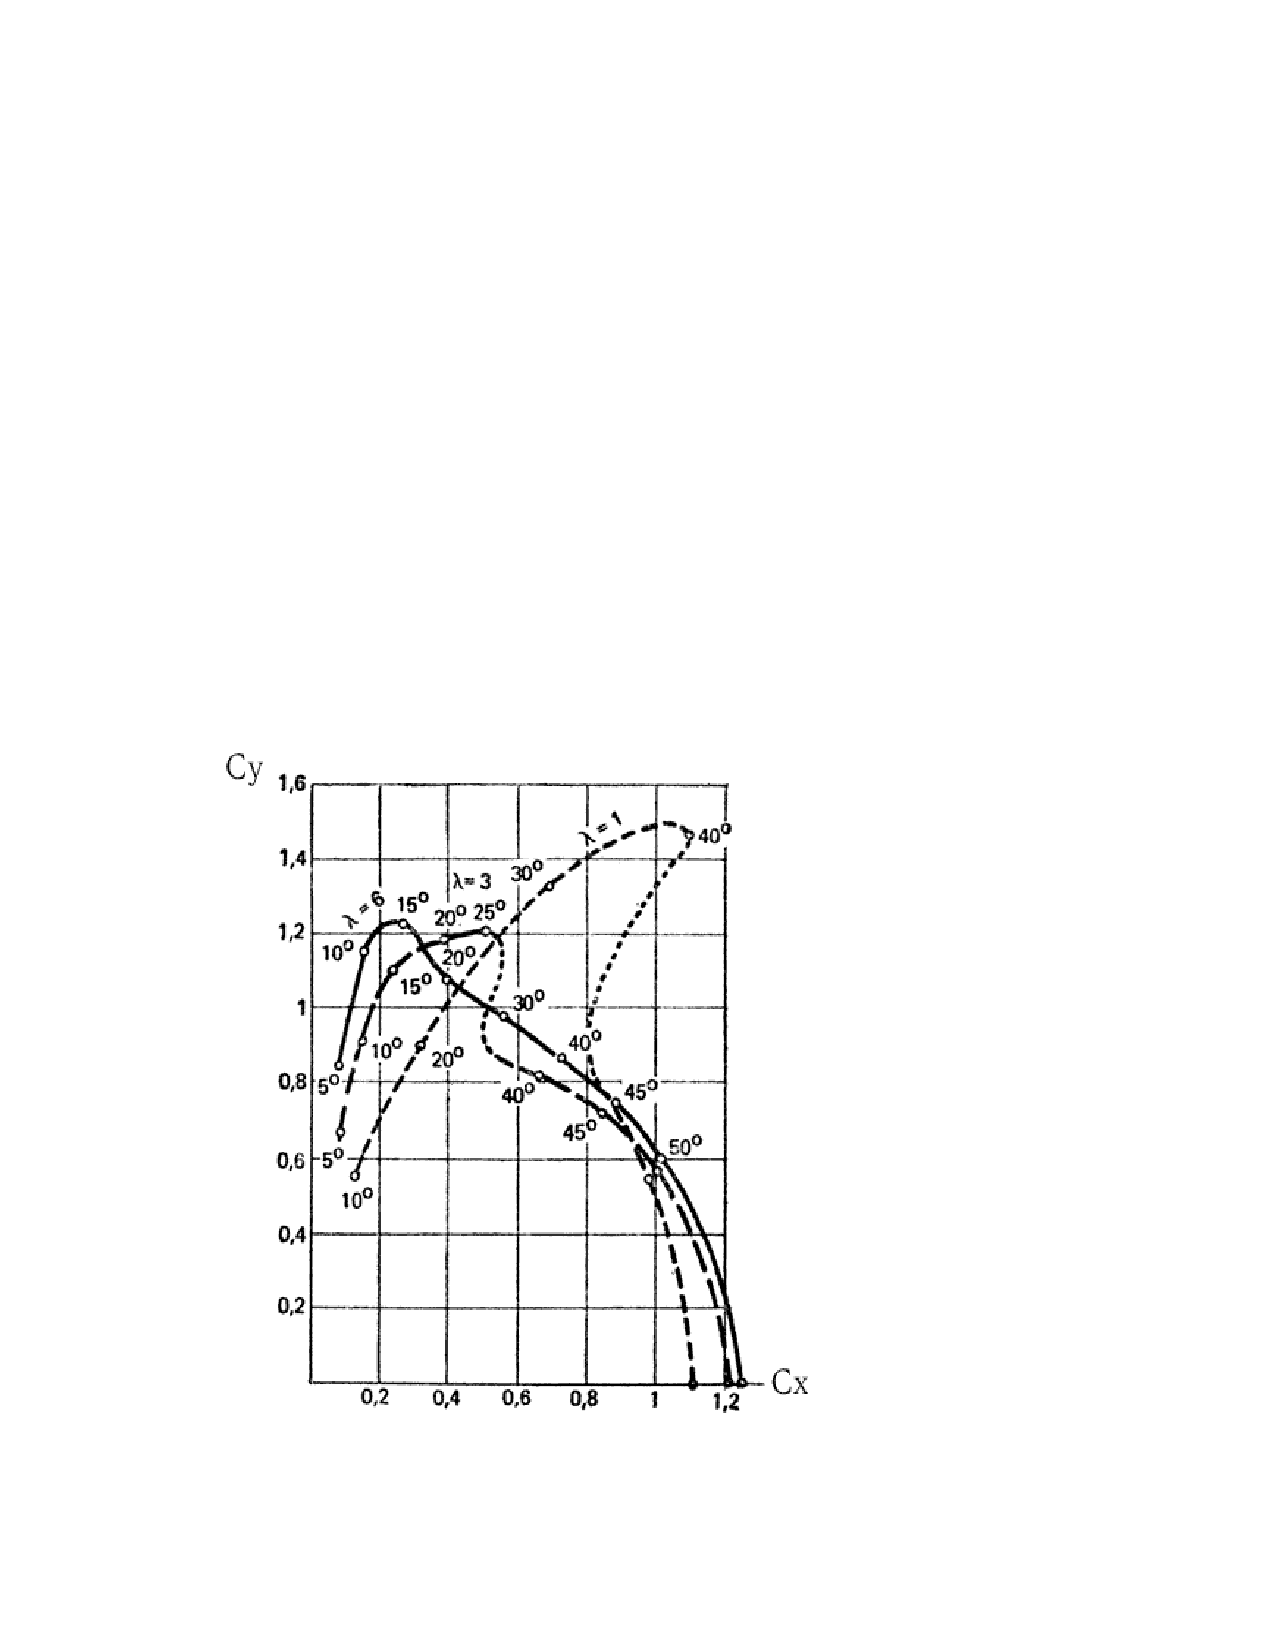
\includegraphics[scale=1]{0028}
  \caption{Поляры трех парусов различного удлинения}
  \label{fig:28}
\end{figure}

Очевидно, что наибольшим индуктивным сопротивлением обладает четырехугольный гафельный парус, у которого перетекание воздуха происходит по верхней и нижней широким кромкам. Поэтому коэффициент подъемной силы здесь резко падает (см. рис.~\ris{8}).

У паруса с эллипсовидной верхней частью величина подъемной силы из-за плавного уменьшения площади паруса у верхнего конца также плавно убывает. Благодаря этому плавно убывает и интенсивность перетекания воздуха через кромки, не происходит местного изменения угла атаки и коэффициента подъемной силы. 

Попытка приблизить форму паруса к эллипсовидной при существующих ограничениях ширины фаловой доски и эластичности мачты была сделана, например, на английском двенадцатиметровике <<Лайонхат>> \--- претенденте на Кубок Америки 1980\,г.: верхняя часть мачты на нем была сильно изогнута. Испытания в аэродинамической трубе показали, что грот с гнутой мачтой дает примерно 10\otdo 30\% увеличения движущей силы по сравнению с обычным бермудским парусом или увеличение скорости лавировки на ветер порядка 4\%.
 
У треугольного паруса основная площадь и, следовательно, нагрузка сосредоточены в нижней трети. По мере приближения к фаловому углу площадь и подъемная сила убывают, что сопровождается соответствующим уменьшением скорости и фактического угла атаки паруса к набегающему потоку. Близ фалового угла также усиливается отрицательный эффект мачты поскольку размеры ее сечения увеличиваются относительно хорды паруса. Эксперименты показали, что если срезать бермудский парус на 15\% высоты от вершины, то практически его тяга не уменьшится. 

Существенное влияние на характеристики паруса оказывает аэродинамическое удлинение паруса (отношение длины передней шкаторины) к его средней хорде, измеренной на половине высоты, или отношение квадрата высоты паруса и его площади.

На рис.~\ris{28} представлены поляры трех парусов различного удлинения --- от $\lambda = 1$ до 6, имеющих одинаковое <<пузо>> $f/b=7,4\%$. Сравнивая поляры можно заметить, что при угле атаки $\alpha = 10\gr$ наивысшую аэродинамическу силу дает парус с максимальным удлинением $\lambda = 6$. Этот же парус имеет наивыгоднейшее направление аэродинамической силы для получения максимальной тяги на курсе бейдевинд. 

Аэродинамическая сила на парус имеющем $\lambda = 6$ достигает максимум при $\alpha = 15\gr$, затем падает. При угле атаки около 35\gr, т. е. на полных курсах, заметное преимущество получай более широкие паруса, имеющие $\lambda = 1$. Таким образом, можно сделать вывод, что парус с большим удлинением при переходе яхты на полный курс становится менее выгодным. На курсе полный бакштаг, например, более быстроходной может оказаться яхта, ocнащенная широкими гафельными парусами с удлинением около 1. Вот почему несмотря на общепризнанное преимущество бермудских парусов, гафельные паруса довольно часто применяют на моторно-парусных яхтах, у которых паруса используются преимущественно при сильных ветрах и на попутных курсах. 

У большинства современных яхт лавировочные паруса имеют отношение длин шкаторин от 3 до 5; паруса для полных курсов \--- дрифтеры, блуперы и спинакеры шьют с соотношением шкаторин, близким к 1.

Пределом для использования парусов большого удлинения является ограниченная остойчивость яхт, не позволяющая чрезмерно повышать положение \textit{ЦП}. Более высокая парусность требует также рангоута большего сечения, что приводит к распространению влияния мачты на большую часть площади грота.

\section{Взаимодействие парусов}

Мы рассматривали особенности \--- аэродинамики одиночного паруса как крыла с тонким поперечным профилем. Большинство яхт, однако, оснащены по крайней мере двумя парусами \--- гротом и стакселем. Поскольку оба паруса расположены в непосредственной близости друг от друга и обтекаются одним потоком воздуха, то естественно предположить наличие их взаимного влияния. 

\begin{figure}[htb]
  \centering
  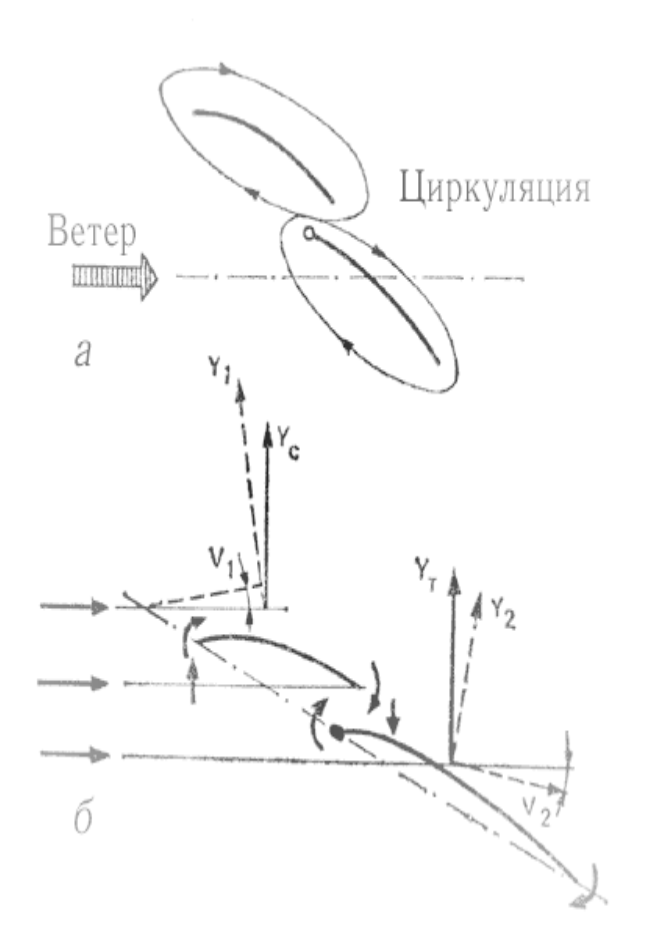
\includegraphics[scale=1]{0029}
  \caption{Циркуляция около пары парусов}
  \label{fig:29}
\end{figure}

До недавнего времени среди яхтсменов пользовалась популярностью теория Вентури, заимствованная из авиации. Согласно этой теории, основным назначением стакселя считалось создание щели \--- сопла между стакселем и гротом, входя в которую, поток воздуха увеличивает свою скорость, способствуя тем самым понижению давления на подветренной стороне грота, особенно в районе, где паруса перерывают друг друга. В результате должна увеличиваться аэродинамическая сила на гроте.

В настоящее время взаимодействие парусов рассматривается на основании вихревой теории крыла \--- исходя из наличия циркуляции вокруг обоих парусов (рис.~\ris{29}). Основная роль в паре грот \--- стаксель принадлежит стакселю. Бесспорно, что воздух, протекающий в щели между гротом и стакселем, имеет повышенную скорость. Однако это прежде всего сказывается на скорости потока, обтекающего подветренную сторону стакселя. Частицы воздуха, вырываясь из щели, увлекают с собой воздух с подветренной стороны стакселя подобно эжектору. Соответственно ускоряется поток вдоль всей подветренной поверхности стакселя, увеличивается циркуляция вокруг его профиля и возрастает аэродинамическая сила. И что еще важно - парус может работать без срыва потока на больших углах атаки.
 
Вызванная скорость (поперечная составляющая вследствие циркуляции) у передней шкаторины грота увеличивает угол атаки, под которым поток натекает на стаксель. Благодаря этому аэродинамическая сила растет и отклоняется вперед \--- на более выгодный угол. На курсе бейдевинд, к слову сказать, большой генуэзский стаксель дает на 30\% большую движущую силу, чем грот, и на 45\% меньшую силу дрейфа.
 
Грот работает в области потока, отклоняемого вызванными скоростями у задней шкаторины стакселя. Это приводит к уменьшению угла атаки грота. Однако воздух, отраженный от стакселя, как бы прилипает к подветренной поверхности грота, благодаря чему предотвращается отрыв от нее пограничного слоя.

Стаксель влияет и на положение критической точки: она перемещается с наветренной стороны мачты ближе к ее передней кромке. В результате уменьшается скорость потока с подветренной стороны грота и сильно снижается пик разрежения у передней шкаторины. Поэтому тенденция к отрыву пограничного слоя и образованию завихрений на гроте ослабевает, парус более эффективно работает на больших углах атаки, чем без стакселя. Скорее этим, а не ускорением потока в щели между гротом и стакселем, по теории Вентури, можно объяснить положительное действие стакселя на работу грота.

Чем больше выбирают стаксель, тем меньше становится разность давлений на подветренной и наветренной сторонах грота. Когда они сравняются, выпуклая форма паруса уже не может поддерживаться \--- парус заполаскивает. Поскольку стаксель более эффективен, чем грот, и дает меньшую кренящую силу, то экипажи крейсерско\-/гоночных яхт уделяют большое внимание подбору стакселей для различных курсов и силы ветра. В гонках при усилении ветра целесообразно уменьшат площадь парусности рифлением грота продолжая по возможности нести стаксель. На отдельных порывах крен можно уменьшать, потравливая грот.

Поскольку Правила обмера IOR прямо не ограничивают длину нижней шкаторины стакселей, то обычно стараются шить их с максимальным перекроем (заходом стакселя за мачту). Существуют, однако, вполне определенные пределы перекроя, далее которых парус теряет свою эффективность и начинает отрицательно влиять на работу грота.

Прежде всего это обеспечение оптимального угла установки стакселя относительно ДП яхты, который равен для лавировки 12\otdo 18\gr. Это труднодостижимо при большой длине нижней шкаторины стакселя и сравнительно небольшой ширине палубы яхты. Как правило, кипы стаксель\-/шкотов удается разместить при несколько меньших углах установки паруса \--- 9\otdo 12\gr. По этому при слишком <<пузатом>> стакселе возможен сток потока воздуха с него на переднюю шкаторину грота и заполаскивание ее по всей высоте. Кроме того, возможно сильное скручивание стакселя: в верхней части ветер будет выдувать из паруса и он перестанет работать. 

\begin{figure}[htb]
  \centering
  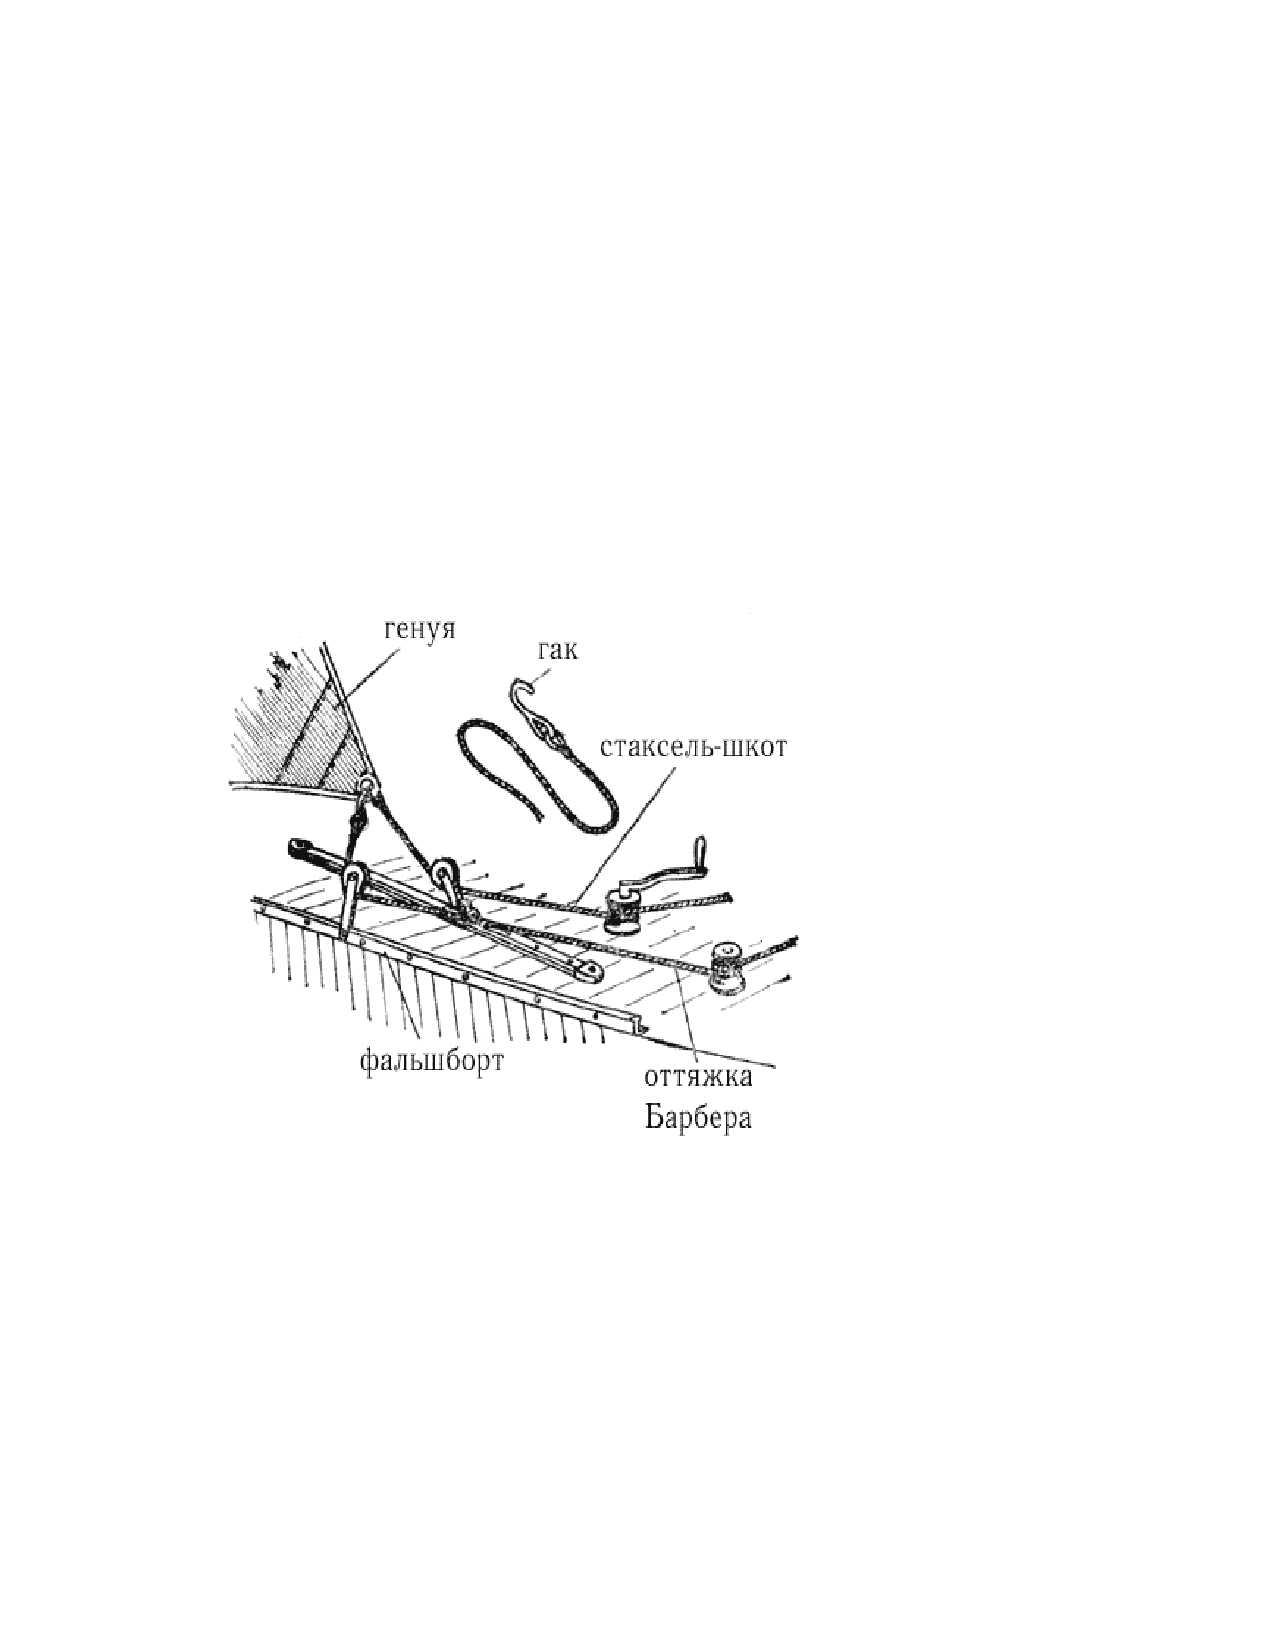
\includegraphics[scale=1]{0030}
  \caption{Оттяжка шкота}
  \label{fig:30}
\end{figure}

Для регулирования положения кип стаксель\-/шкотов в зависимости от величины стакселя и курса относительно ветра используют специальный фальшборт из металлического угло\-/бульбового профиля с большим числом отверстий или крепят кипы на передвижных ползунах, скользящих по прочному палубному рельсу. При настройке стакселя стараются получить равномерный зазор между гротом и стакселем по всей высоте и <<пузо>> стакселя, смещенное к передней шкаторине. При перемещении кипы вперед тяга шкота сильнее натягивает заднюю шкаторину. В результате <<пузо>> увеличивается по всей площади, парус меньше скручивается, но возможно заворачивание задней шкаторины на ветер. При перемещении кипы назад, увеличивается натяжение нижней шкаторины; натяжение задней шкаторины будет недостаточным, парус сильно скрутится и может заполаскивать в верхней части. Иногда полезно применить дополнительную снасть \--- оттяжку шкота (рис.~\ris{30}) для осаживания задней шкаторины. Выбрав втугую парус по нижней шкаторине за шкот, с помощью оттяжки добиваются нужного натяжения задней шкаторины и положения <<пуза>> по ширине паруса, устраняют сильное скручивание. Правильно отрегулированный стаксель должен давать поток воздуха, направленный по касательной к поверхности грота и при приведении яхты заполаскивать сразу по всей высоте. Хорошую службу при настройке могут оказать индикаторы (см. рис.~\ris{22}--\ris{23}).

Большое влияние на полноту стакселя оказывает прогиб штага. Чем сильнее при усилении ветра прогибается штаг, тем больше становится <<пузо>> паруса и он начинает задувать на грот. В известной мере прогиб компенсируется специальным раскроем стакселя с выпуклостью в нижней части передней шкаторины и вогнутостью (отрицательным серпом) в верхней. Многие яхты за рубежом снабжают мощными гидравлическими, винтовыми устройствами или талями для увеличения натяжения ахтерштага и даже наклона мачты назад.

\section{Лобовое сопротивление яхты}

Влияние лобового (воздушного) сопротивления яхты на ее ходовые качества исключительно велико. На курсе бейдевинд при ветре 4 балла на преодоление воздушного сопротивления яхты затрачивается около одной трети силы тяги, развиваемой парусами. Поэтому снижение лобового сопротивления так же важно, как и снижение сопротивления воды.

В общем балансе воздушного сопротивления на долю парусов и рангоута приходится 70\otdo 78\%, такелажа \--- 3\otdo 5\%, корпуса \--- 15\otdo 18\%, экипажа \--- 4\otdo 6\%. Поскольку основную роль играют паруса и рангоут, рассмотрим причины, обусловливающие появление на них сил сопротивления.

Воздушное сопротивление, как и сопротивление воды, считают возможным разделить на несколько компонентов. Для парусов их два: индуктивное сопротивление и сопротивление формы (или профильное). Как мы уже говорили, индуктивное сопротивление является неизбежным следствием действия на парусе аэродинамической подъемной силы. По мере роста скорости вымпельного ветра и соответственно величины подъемной силы растет и величина индуктивного сопротивления. В средний ветер в области оптимальных углов атаки паруса ($\alpha = 5\motdo 15\gr$) индуктивное сопротивление существенно выше сопротивления формы. Проявляется оно в виде двух вихревых дорожек, стекающих с нижней шкаторины и близ фалового угла паруса.
 
Основные факторы, влияющие на индуктивное сопротивление, \--- аэродинамическое удлинение и форма парусов, угол скручивания и распределение <<пуза>> по высоте паруса. Чем больше удлинение паруса (т.\=,е. чем меньше относительно высоты паруса длина нижней шкаторины и верхней части паруса, через которые происходит перетекание воздуха из зоны повышенного давления на сторону разрежения), чем ближе к форме эллипса форма верхней части паруса, тем меньше индуктивное сопротивление. От угла скручивания и величины <<пуза>> в верхней части паруса зависит величина подъемной силы и ее распределение на этом участке. У треугольного бермудского паруса в верхней части желательно получить большую подъемную силу на единицу площади, чем на середине высоты мачты, потому что тогда характер распределения нагрузки приближается к эллиптическому крылу, имеющему минимальное индуктивное сопротивление. Вот почему в верхней части паруса часто выкраивают с несколько большим <<пузом>>, а скручивание паруса допускается лишь на незначительные углы. Корпус яхты, в непосредственной близости от которого располагаются нижние шкаторины парусов, является своеобразной аэродинамической шайбой, в известной мере снижающей перетекание воздуха через нижние шкаторины. 

Профильное сопротивление парусов, в свою очередь, можно разделить на сопротивление трения и давления. Сопротивление трения вызвано вязкими свойствами воздуха и подчиняется тем же законам, что и сопротивление трения воды, хотя коэффициент кинематической вязкости воздуха в 860 раз меньше, чем воды. Нормальным режимом обтекания парусов является турбулентный, при котором коэффициент сопротивления трения в большой степени зависит от степени гладкости поверхности. Более ворсистые и имеющие крупную текстуру хлопчатобумажные ткани обладают большим сопротивлением трения, чем лавсановые или дакроновые, особенно пропитанные смолой. 

Сопротивление трения повышается при наличии на парусах большого количества швов, поперечных морщин складок, различных нашивок. Особенно важно иметь гладкую поверхность близ передней шкаторины паруса, где возможно ламинарное обтекание и где формируется поток вдоль подветренной стороны паруса. Наличие здесь морщин или нашивок способствует турбулизации потока и его отрыву от поверхности паруса, в результате чего падает подъемная сила. 

Сопротивление давления зависит от формы поперечного сечения \--- профиля паруса и угла атаки его относительно вымпельного ветра. Очевидно, что сопротивление плоской пластины при нулевом угле атаки во флюгерном положении будет полностью обусловлено трением. По мере увеличения угла атаки появится дополнительное сопротивление, которое при расположении пластины перпендикулярно потоку будет максимальным и полностью представит собой сопротивление давлений. Если при $\alpha = 0\gr$ коэффициент сопротивления пластины $C_X = 0,004\motdo 0,008$, то при $\alpha = 90\gr$ $C_X = 1,9$. Это означает, что сопротивление давления может в 250\otdo 500 раз превышать сопротивление трения, однако влияние трения на режим обтекания паруса и его подъемную силу заставляет парусных мастеров экипажа яхты уделять качеству отделки парусов достаточно большое внимание.

Сопротивление давления паруса, имеющего <<пузо>>, при малых углах атаки превышает сопротивление плоской пластины. Чем больше относительная величина <<пуза>> и чем дальше передней кромки оно располагается, тем больше профильное сопротивление. На его величине сильно сказываются искажения правильного профиля \--- складки, слишком туго набитые в карманах латы, свободно болтающаяся или, наоборот, слишком перебранная задняя шкаторина и т.\=,п.
 
О вредном, но неизбежном влиянии мачты на тяговые характеристики паруса мы уже говорили. Кроме того, мачта сама по себе является далеко не идеально обтекаемым телом, обладает довольно значительным профильным сопротивлением, которое возрастает с увеличением скорости ветра. Немало случаев, когда в сильный попутный ветер яхта под одним рангоутом развивает достаточную скорость, чтобы слушаться руля.

Иное дело обтекатели штага, снабженные ликпазом, которые в последнее время все чаще находят применение на крейсерско\-/гоночных яхтах (см. рис.~\ris{46}). Выполняемые обычно в виде хорошо обтекаемого алюминиевого или пластикового профиля с толщиной, равной 24\otdo 29\% хорды, они примерно на 20\% снижают профильное сопротивление стакселя и на 5\% повышают его подъемную силу. Главный эффект состоит в оформлении и утолщении входящей кромки стакселя как аэродинамического профиля. Критическая точка (см. рис.~\ris{22}) перемещается ближе к подветренной стороне обтекателя, благодаря чему пик разрежения вблизи передней шкаторины становится плавнее и достигается при несколько больших углах атаки. Кроме того, обтекатели способствуют уменьшению прогиба штага, отрицательно влияющего на профиль паруса.

В отличие от сопротивления парусa, создающего движущую силу, сопротивление мачты, краспиц, гика, стоячего и бегучего такелажа относят к так называемому паразитному сопротивлению. Оно занимает 10\otdo 12\% общего воздушного сопротивления, поэтому сокращение длины и уменьшение диаметра всех тросов на яхтах очень важно. Мачты желательно <<очистить>> от большинства фалов и электропроводки, убрав их внутрь. По возможности внутри мачты следует расположить крепления стоячего такелажа и блоки фалов.

\section{Ходовые качества яхты на различных курсах}

\begin{figure}[hbt]
  \centering
  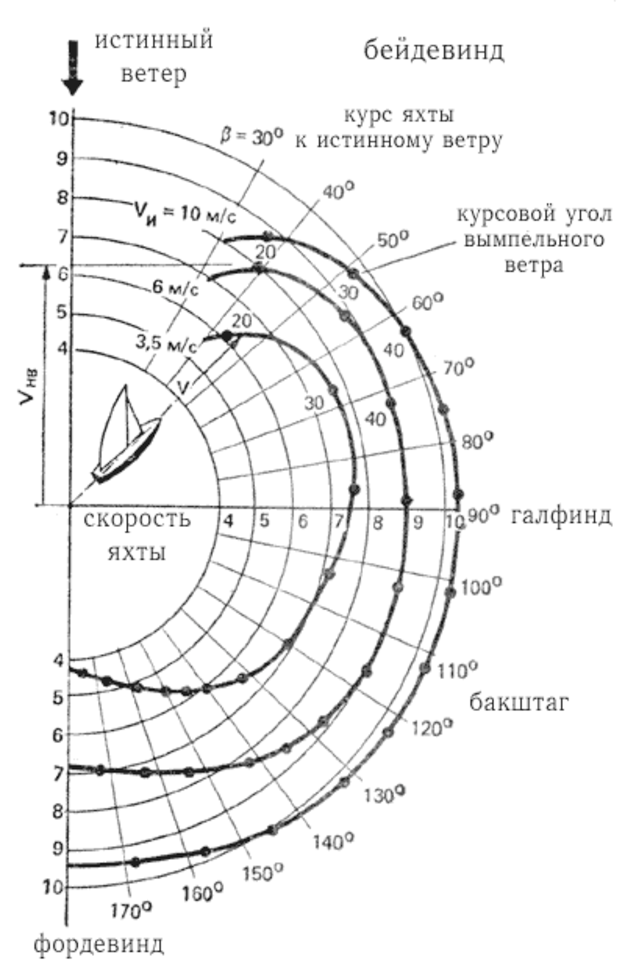
\includegraphics{0031}
  \caption{Полярная диаграмма ходкости яхты}
  \label{fig:31}
\end{figure}

Появившиеся в оснащении яхт приборы позволяют измерять параметры их движения и на основе этих измерений оценивать ходовые качества судна на разных курсах по отношению к ветру количественно, а не <<на глазок>>. Наиболее доступные приборы дают следующую информацию:

\begin{itemize}
\item угол между \textit{ДП} яхты и направлением вымпельного ветра; 
\item скорость вымпельного ветра; 
\item скорость яхты относительно воды; 
\item мгновенное изменение скорости яхты относительно выбранной точки отсчета. 
\end{itemize}

Пользуясь показаниями этих приборов, экипаж может оптимальным образом настроить паруса для каждого курса, чтобы получить наивысшую скорость, а также построить полярную диаграмму ходкости яхты (рис.~\ris{31}). При построении диаграммы яхта считается расположенной в центре нескольких концентрических окружностей, каждая из которых соответствует определенной скорости (4, 5, 6 и т.\=,д. уз). Из центра через 10\gr проводятся лучи, обозначающие курсы яхты по отношению к направлению истинного (или вымпельного) ветра. Для удобства в правой части диаграммы могут быть нанесены курсы судна относительно направления истинного, а по левую \--- относительно вымпельного ветра. Затем на каждом луче откладывается значение оптимальной скорости на данном курсе и при данной силе ветра.

Нетрудно заметить, что поляра скорости яхты на курсе от полного бейдевинда до крутого бакштага близка к дуге окружности, иными словами, с изменением курсового угла ветра скорость меняется очень незначительно. При переходе яхты на чистый фордевинд скорость заметно падает, особенно в слабый ветер. Объясняется это существенным снижением скорости вымпельного ветра и, поскольку аэродинамические силы пропорциональны ее квадрату, уменьшением силы тяги.

Постановка дополнительных парусов \--- спинакера и блупера помогает увеличить скорость яхты в слабый и средний ветер. В сильный же ветер, когда скорость оказывается близкой к предельной, $v = 3 \cdot {\lkvl}^{1/2}$, уз. и кривая сопротивления воды круто поднимается вверх, увеличение силы тяги при увеличении парусности практически не дает повышения скорости. На курсе бейдевинд скорость вымпельного ветра и аэродинамические силы максимальные, однако подъемная сила дает очень небольшую составляющую в направлении движения яхт (см. рис.~\ris{20}). С увеличением же на этом курсе крена уменьшается эффективный угол атаки относительно вымпельного ветра, падает величина аэродинамической силы и силы тяги. По этому на острых курсах более остойчивая яхта может оказаться быстроходней. 

С помощью полярной диаграммы рулевой яхты может решать различные тактические задачи, например выбрать оптимальный курс в лавировку. Он определяется по наибольшей скорости продвижения прямо против ветрa. Для этого следует провести касательную к поляре для данной силы ветра \--- перпендикуляр к его направлению. Точка касания поляры указывает наиболее выгодный курс. При плавании полным курсом, зная расстояние до конечной точки, можно с помощью поляры определить, как выгоднее будет пройти дистанцию \--- курсом фордевинд или двумя бакштагами со сменой галса.

Для того чтобы облегчить возможность использования полярной диаграммы, на кривых скорости наносят курсы яхты относительно вымпельного ветра. Получаются они построением треугольника скоростей по данным снятым с диаграммы (см. рис.~\ris{19}, \textit{б}) поскольку с движущейся яхты определить направление истинного ветра можно только приближенно \--- с помощью компаса и волны либо по береговым приметам.

\chapter{Некоторые особенности конструкции крейсерско-гоночных яхт}

\section{Классификация и основные требования, предъявляемые к крейсерско-гоночным яхтам}

Яхты для дальних плаваний (крейсерские яхты) можно разделить на три основные группы, отличающиеся по своему назначению: крейсерско\-/гоночные, крейсерские и туристские. 
Основным назначением \textbf{крейсерско\-/гоночных} яхт (их правильнее было бы называть гоночными яхтами открытого моря) является успешное выступление в маршрутных гонках на длинные дистанции. Крейсерско\-/гоночные яхты имеют характерное парусное вооружение с узкими и высокими парусами, свободную палубу, насыщенную механизмами и устройствами для управления парусами и их настройки (рис.~\ris{32}). Типичными представителями этой группы яхт являются, например, однотонник <<Марина>>, яхты <<Конрад-44>> и <<Конрад-54>>.

\begin{figure}[htb]
  \centering
  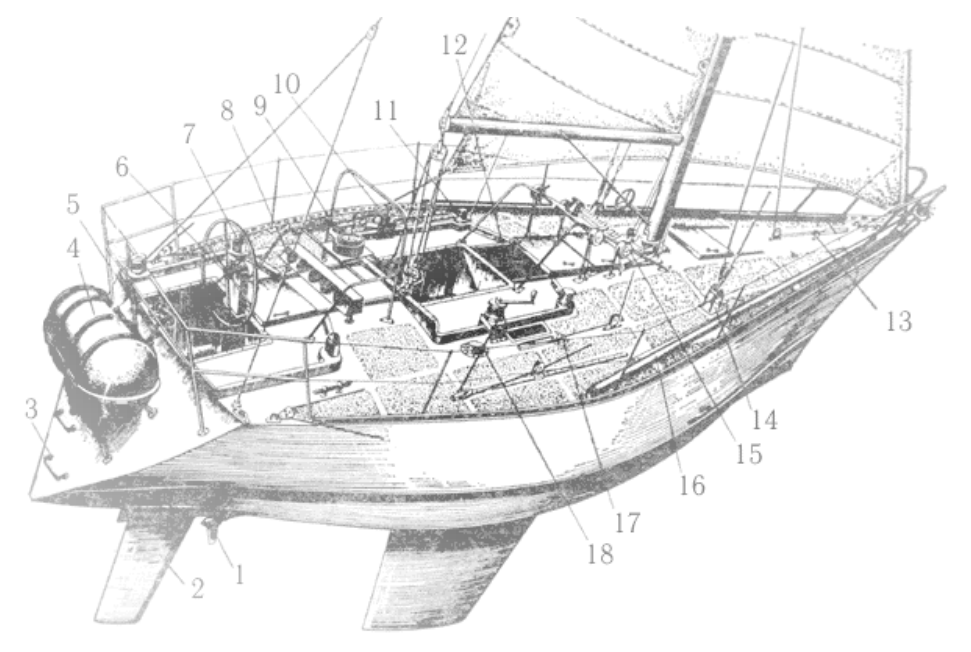
\includegraphics{0032}
  \caption{Однотонник <<Марина>> постройки ленинградской судоверфи ВЦСПС}
  \label{fig:32}
  \small
  \centering{}
  1 \--- гребной винт регулируемого шага; 2 \--- перо руля; 3 \--- скоб\-/трап; 4 \--- надувной спасательный плот ПСН-6М; 5 \--- привод натяжного ахтерштага; 6 \--- штурвал; 7 \--- путевой компас; 8 \--- приборная панель; 9 \--- главный компас; 10 \--- двухскоростная лебедка; 11 \--- односкоростная лебедка; 12 \--- входной люк; 13 \--- натяжка внутреннего штага; 14 \--- вант\-/путенс; 15 \--- фаловая лебедка; 16 \--- спинакер\-/гик; 17 \--- натяжка багштага; 18 \--- вентиляционный дефлектор
\end{figure}

\textbf{Крейсерские яхты} \--- достаточно быстроходные суда, используемые для дальних спортивных плаваний определенной категории сложности и протяженности. Суда этого типа принимают также участие в морских гонках, хотя и с меньшими шансами на успех при выступлении в одной зачетной группе с гоночными яхтами. Крейсерские яхты, рассчитанные на многодневное пребывание экипажа на борту, имеют лучшие условия обитаемости, большие запасы пресной воды и топлива, часто снабжаются более мощным двигателем. Такие суда имеют палубные рубки, позволяющие увеличить объем внутренних помещений и их высоту; конструкцию корпуса, отвечающую правилам постройки классификационных обществ. При больших измерениях они оснащаются двухмачтовым вооружением. К судам этой группы можно, например, отнести однотонник, построенный небольшой серией на таллинской экспериментальной верфи спортивного судостроения, яхты типа <<Конрад-45>> и <<Опал>>.

\textbf{Туристские яхты} \--- мореходные и комфортабельные суда, рассчитанные на длительное плавание, не лимитируемое нормативами времени. Они оснащаются низким парусным вооружением с относительно небольшой площадью парусности, часто стилизуются под старинные кечи, шхуны и тендера. Мощный двигатель и топливные цистерны большой емкости позволяют получить высокую скорость и значительную дальность плавания под двигателем. По скорости и лавировочным качествам они уступают крейсерским. 

В зависимости от мощности двигателя, установленного на яхте, ее можно классифицировать как яхту парусно\-/моторную \--- со вспомогательным двигателем или как моторно\-/парусную. В первом случае мощность двигателя составляет 1,5\otdo 2,5~л.с. на каждую тонну полного водоизмещения яхты, что обеспечивает достижение скорости от 5 до 6 уз. По запасу топлива для двигателя яхта имеет дальность плавания 80\otdo 120 миль; используются гребные винты со складывающимися лопастями или флюгерного типа, оказывающие минимальное сопротивление движению яхты под парусами. Двигатель служит лишь для выхода из гавани и входа в нее, для коротких переходов в штилевых условиях и в аварийных ситуациях, а также для подзарядки аккумуляторных батарей. 

На моторно\-/парусных яхтах удельная мощность двигателя достигает 5\otdo 8~л.с./т.; запасы топлива для него принимаются из расчета обеспечения дальности плавания в несколько сотен миль со скоростью 8\otdo 10~уз. Устанавливаются эффективные трехлопастные гребные винты большого диаметра, оказывающие на ходу под парусами большое сопротивление движению. Наличие тяжелого двигателя и запасов топлива обусловливает уменьшение массы балласта до 15\otdo 25\% водоизмещения яхты, что, в свою очередь, заставляет ограничивать площадь парусности. Моторные парусники \--- это туристские яхты, у которых двигатель является таким же, если не более важным средством движения, как и паруса. 

По району плавания крейсерские яхты делятся на яхты для внутренних вод, озерного и прибрежного морского плавания и яхты для открытого моря (океанские). 

Для плавания по относительно закрытым внутренним водам, характерным невысокой волной и наличием большого числа пунктов, в которых яхта может укрыться от непогоды, мореходность яхт может быть ограничена, корпус, рангоут и такелаж могут иметь легкую конструкцию. Оптимальными типами судов для плавания по внутренним водам являются крейсерские швертботы, компромиссы, яхты с тяжелым подъемным килем и небольшие килевые суда, осадка которых не превышает 1,4~м. Поскольку при дальних спортивных плаваниях и гонках такие суда выходят в довольно обширные водохранилища с неприятной крутой волной, яхты для внутренних вод следует снабжать самоотливными кокпитами, предусматривать надежные закрытия входных и светлых люков и обеспечивать положительную остойчивость при крене до 90\gr \--- возможность самовыпрямления в аварийных ситуациях. 

Яхты, предназначенные для прибрежного морского и озерного плавания, должны быть рассчитаны на достаточно длительное противодействие сильному ветру и крупной волне и способность отлавировать от подветренного берега. Для таких судов обязателен самоотливной кокпит, прочный рангоут и такелаж, каюта достаточного объема, оборудованная койками для отдыха экипажа, работоспособный на волне камбуз, штурманский стол для ведения прокладки и компас. 

Наиболее жесткие требования к мореходности, оборудованию и снабжению предъявляются к яхтам открытого моря. 

Для судов, участвующих в гонках, эти требования дифференцируются в зависимости от сложности маршрута \--- категории гонок. 

Самые крупные и мореходные яхты, называемые неофициально яхтами нулевого класса, или макси\-/яхтами, имеют гоночный балл по правилам IOR, близкий к максимально допустимому значению 19\otdo 22~м. Такие суда строятся почти исключительно для трансокеанских и кругосветных гонок. Они рассчитываются на достижение максимально возможных скоростей на трассах с попутными ветрами с тем, чтобы ликвидировать преимущество, которое дает гандикап меньшим по размерам яхтам. Наибольшая длина макси\-/яхт составляет 21\otdo 24~м; длина по КВЛ \--- около 19~м; ширина \--- около 5,5~м; водоизмещение \--- 30\otdo 35~т; масса балластного фальшкиля \--- 16\otdo 18~т; осадка \--- до 3,6~м; обмерная площадь парусности \--- около 240~м$^2$. В гонках экипаж таких яхт состоит из 13\otdo 17 человек. Корпуса их строятся из алюминиевых сплавов, реже \--- из стеклопластика или деревянной конструкции. 

Наиболее многочисленную группу яхт на любых гонках составляют яхты длиной от 10 до 12,5 м (III\--II классов IOR). Среди них имеется немало сравнительно дешевых однотипных судов, построенных по одному проекту что позволяет в ряде случаев выделить их в отдельные стартовые группы и повысить интерес экипажей к соревнованиям.
Дальнейшим развитием типизации является введение так называемых <<тонных>> или <<уровневых>> классов яхт, которые строятся по специальным правилам. Основным признаком для деления на классы служит величина гоночного балла IOR. Таких классов шесть: <<двухтонники>> (с гоночным баллом не более 32 футов \--- 9,76~м); <<однотонники>> (27,5 фута \--- 8,38~м); <<3/4-тонники>> (24,5 фута \--- 7,47 м); <<полутонники>> (21,7 фута "--- 6,60~м); <<четвертьтонники>> (18,5 фута \--- 5,65~м) и <<минитонники>> (16,5 фута \--- 5,18 м). Для каждого из этих классов имеются специальные требования к планировке корпуса, оборудованию и т.\=,п. Это типичные гоночные яхты ограниченной обитаемости, хотя участвуют в гонках на дистанциях 150\otdo 400 миль. Они могут выступать и в соревнованиях с яхтами других типов с учетом гандикапа.

Основным требованием, предъявляемым к крейсерско\-/гоночным яхтам, является их высокая эффективность в гонках при высоких мореходных качествах. 

Высокий надводный борт, большая ширина корпуса и значительная масса балласта (40\otdo 50\%) позволяют обеспечить достаточную остойчивость яхты для несения эффективной парусности в сильный ветер. Единственно приемлемым типом вооружения для крейсерско\-/гоночных яхт малых и средних размеров является бермудский шлюп благодаря его высоким аэродинамическим качествам. Яхта оснащается большим числом вспомогательных парусов, средств для их настройки, позволяющих получить максимальную тягу при ветре любой силы и на любом курсе яхты по отношению к нему. Работу экипажа с парусами облегчают палубные шкотовые и фаловые лебедки, стопора, оттяжки и т.\=,п. 

\begin{figure}[htb]
  \centering
  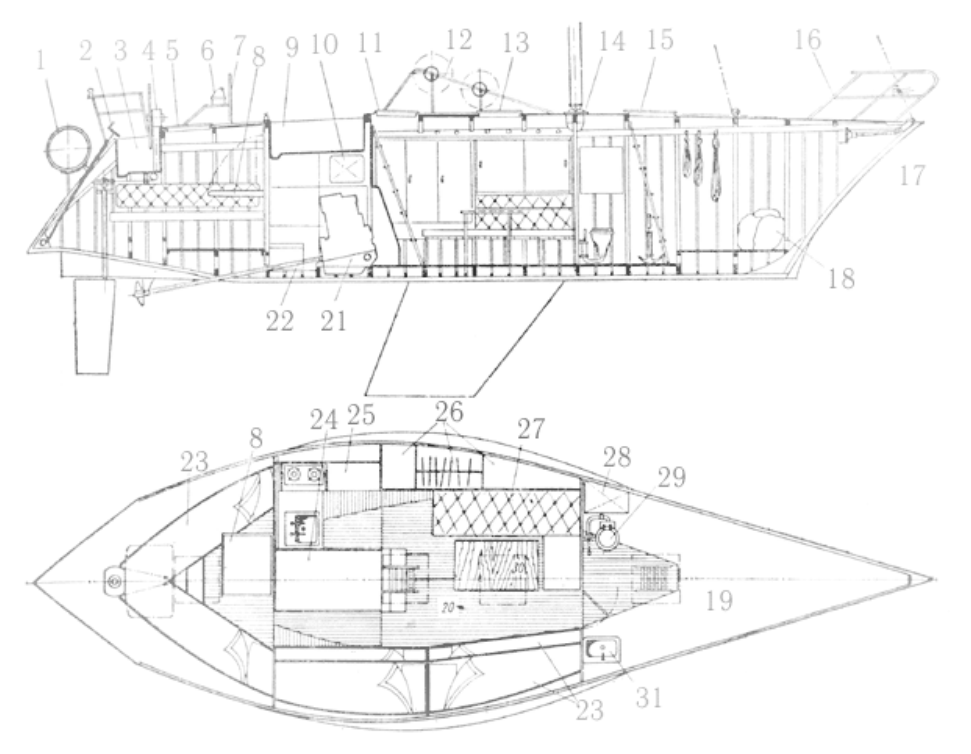
\includegraphics{0033}
  \caption{Общее расположение однотонника <<Марина>>}
  \label{fig:33}
  \small
  \centering{}
  1 \--- спасательный плот; 2 \--- привод натяжки ахтерштага; 3 \--- кокпит рулевого; 4 \--- колонка штурвала; 5 \--- ахтерлюк; 6 \--- путевой компас; 7 \--- поручень\-/стойка компаса; 8 \--- штурманский стол; 9 \--- кокпит шкотовых; 10 \--- топливный бак; 11 \--- входной люк; 12 \--- стойка лебедок и стопоров; 13 \--- светлый люк; 14 \--- степс; 15 \--- форлюк; 16 \--- носовой релинг; 17 \--- натяжка штага; 18 \--- паруса; 19 \--- форпик; 20 \--- салон; 21 \--- двигатель; 22 \--- аккумуляторы; 23 \--- конки; 24 \--- моторное отделение; 25 \--- камбуз; 26 \--- шкафы; 27 \--- диван; 28 \--- цистерна питьевой воды; 29 \--- унитаз; 30 \--- стол; 31 \--- умывальник. 
\end{figure}

Крейсерско\-/гоночную яхту стараются оборудовать электронными приборами, облегчающими навигацию и ведение гонки. В их комплект входят эхолоты, лаги, указатели скорости и направления вымпельного ветра, курса яхты относительно него, радиопеленгаторы. На крупных и дорогих яхтах за рубежом не редкость специальные системы радионавигации <<Декка>>, <<Лоран>> и <<Омега>> и даже аппаратура для определения места с помощью искусственных спутников Земли. Большинство яхт снабжаются двумя\-/тремя радиостанциями УКВ и KB диапазонов для связи с берегом и судейским судном при участии в гонке. 

\section{Общее расположение и конструкция корпуса}

Обитаемости крейсерско-гоночных яхт должно уделяться достаточно внимания.

Типичным для гоночных яхт является общая компоновка и планировка внутренних помещений на яхте типа <<Марина>> (см. рис.~\ris{32} и \ris{33}). Характерной является палуба, свободная от рубок и надстроек, что диктуется необходимостью обеспечить удобство работы экипажа с парусами, а также снизить воздушное сопротивление, что важно при лавировке против сильного ветра. Для того чтобы получить нужную высоту внутри каюты, корпус яхты выполнен с повышенным бортом и значительной поперечной погибью палубы.

Гладкопалубный тип утвердился на яхтах меньших размерений вплоть до <<минитонников>>. Однако в большинстве случаев для того чтобы выдержать регламентируемую правилами классов высоту помещения, у входа устанавливается небольшая рубка, совмещенная с входным люком. 

Функционально размещение экипажа в двух кокпитах \--- рулевого в кормовом у самого транца и шкотовых \--- в кокпите близ миделя. Располагаясь позади всего экипажа, рулевой контролирует его действия, имеет хороший обзор парусов, а шкотовые не создают ему помех. Дифферентовка яхты в меньшей степени зависит от числа людей в кокпите, так как он находится ближе к общему центру тяжести судна, чем при традиционном кормовом расположении.

Под палубой экипаж располагается, по существу, в одном большом помещении в средней части яхты. Поперечная переборка, установленная под мачтой, отделяет форпик, используемый в качестве парусной кладовой. Здесь же размещены унитаз с принудительной прокачкой и небольшая раковина. 

Кают\-/компания, она же и каюта для отдыха, оборудована мебелью облегченной конструкции и газовым камбузом. Здесь же, близ центра тяжести яхты, установлен вспомогательный дизель, благодаря чему существенно снизилось его влияние на период килевой качки и соответственно уменьшился прирост сопротивления при лавировке против волны.

В кормовой части судна, отделенная легкой полупереборкой, расположена штурманская каюта со спальными местами для капитана и старшего помощника. Для оперативной связи штурмана или вахтенного начальника, ведущего прокладку по карте, с рулевым предусмотрен открывающийся светлый люк у переднего комингса рулевого кокпита.

Несколько иные принципы планировки общего расположения 15,3\--метровой яхты, рассчитываемой на длительные гонки и плавания в океане. Обеспечению комфорта для экипажа в данном случае уделяется больше внимания. Легкими переборками внутренний объем яхты делится на семь отсеков, или кают. Фор\-- и ахтерпики используются в качестве шкиперских кладовых. Паруса хранятся в носовом кубрике и в тамбуре перед мачтой, куда они подаются с палубы через сдвижной люк. 

Полная вместимость яхты по числу спальных мест составляет 13 человек, но трубчатые койки в носовом кубрике и над парусным рундуком используются только на стоянке и в тихую погоду. Наиболее комфортабельное помещение \--- кормовая трехместная каюта (для владельца или капитана) расположено в непроходной части и через небольшой лючок сообщается с кокпитом рулевого.

Кают\-/компания, камбуз и штурманская рубка расположены вблизи центра тяжести яхты, где меньше ощущается килевая качка и удары волн. Здесь же установлен вспомогательный дизель, закрытый звукоизолирующим капотом, под пайолами расположены цистерны с запасами топлива и питьевой воды.

Двухместная каюта в носовой части яхты может быть использована для размещения вахтенных начальников или гостей. 

\begin{figure}[htb]
  \centering
  \includegraphics{0034-1}
  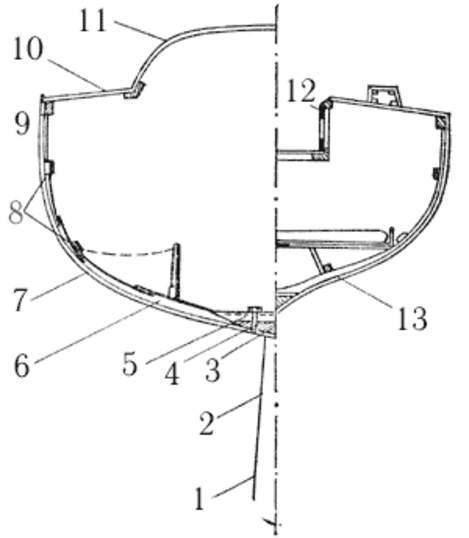
\includegraphics{0034-2}
  \caption{Конструктивный мидель-шпангоут}
  \label{fig:34}
  \small
  \centering{}
а \--- пластмассовой яхты длиной 13,2 м; б \--- яхты деревянной конструкции длиной 12,8 м; 

1 \--- внутренний свинцовый балласт 2,73~т; 2 \--- плавник киля, сварной из стальных листов $\delta = 6$~мм; 3 \--- киль $90 \times 460$ мм; 4 \--- болт М25; 5 \--- флор, сталь $\delta = 6$~мм; 6 \--- ламинированный шпангоут $65 \times 125$~мм, клеенный из пяти реек по толщине; 7 \--- обшивка из семи слоев 3-миллиметрового шпона древесины каури (сорт красного дерева); 8 \--- стрингеры $25 \times 50$~мм; 9 \--- привальный брус $50 \times 75$~мм; 10 \--- палуба, три слоя фанеры толщиной по 6,4~мм; 11 \--- рубка, 7 слоев шпона каури $\delta = 3$~мм. 
\end{figure}


\chapter{Правила обмера крейсерско-гоночных яхт}\label{chap:4}

\end{document}

% Переход на NCC